% Format teze zasnovan je na paketu memoir
% http://tug.ctan.org/macros/latex/contrib/memoir/memman.pdf ili
% http://texdoc.net/texmf-dist/doc/latex/memoir/memman.pdf
% 
% Prilikom zadavanja klase memoir, navedenim opcijama se podešava 
% veličina slova (12pt) i jednostrano štampanje (oneside).
% Ove parametre možete menjati samo ako pravite nezvanične verzije
% mastera za privatnu upotrebu (na primer, u b5 varijanti ima smisla 
% smanjiti 
\documentclass[12pt,oneside]{memoir}

% Paket koji definiše sve specifičnosti mastera Matematičkog fakulteta
\usepackage{assets/matfmaster}

%
% Podrazumevano pismo je ćirilica.
%   Ako koristite pdflatex, a ne xetex, sav latinički tekst na srpskom jeziku
%   treba biti okružen sa \lat{...} ili \begin{latinica}...\end{latinica}.
%
% Opicija [latinica]:
%   ako želite da pišete latiniciom, dodajte opciju "latinica" tj.
%   prethodni paket uključite pomoću: \usepackage[latinica]{matfmaster}.
%   Ako koristite pdflatex, a ne xetex, sav ćirilički tekst treba biti
%   okružen sa \cir{...} ili \begin{cirilica}...\end{cirilica}.
%
% Opcija [biblatex]:
%   ako želite da koristite reference na više jezika i umesto paketa
%   bibtex da koristite BibLaTeX/Biber, dodajte opciju "biblatex" tj.
%   prethodni paket uključite pomoću: \usepackage[biblatex]{matfmaster}
%
% Opcija [b5paper]:
%   ako želite da napravite verziju teze u manjem (b5) formatu, navedite
%   opciju "b5paper", tj. prethodni paket uključite pomoću: 
%   \usepackage[b5paper]{matfmaster}. Tada ima smisla razmisliti o promeni
%   veličine slova (izmenom opcije 12pt na 11pt u \documentclass{memoir}).
%
% Naravno, opcije je moguće kombinovati.
% Npr. \usepackage[b5paper,biblatex]{matfmaster}


% Paket koji obezbeđuje ispravni prikaz ćiriličkih italik slova kada
% se koristi pdflatex. Zakomentarisati ako na sistemu koji koristite ovaj
% paket nije dostupan ili ako ne radi ispravno.
\usepackage{cmsrb}


% Ostali paketi koji se koriste u dokumentu
\usepackage{listings} % listing programskog koda
\usepackage{float}
\setsecnumdepth{subsubsection}
\usepackage{amsmath}
\usepackage{longtable}

\hyphenation{re-di-rec-tion Fa-ce-book me-na-ge-ment Stra-va Stra-vaActivity mi-grate REpresentatio-nal}
% Datoteka sa literaturom u BibTex tj. BibLaTeX/Biber formatu
\bib{master_thesis}

% Ime kandidata na srpskom jeziku (u odabranom pismu)
\autor{Ивона Милутиновић}
% Naslov teze na srpskom jeziku (u odabranom pismu)
\naslov{Развој апликације за асистенцију вежбачима ослањањем на корисничке податке употребом \textit{Аndroid} и \textit{Django} оквира}
\godina{2024}
\mentor{др Иван \textsc{Чукић}, доцент \\
Универзитет у Београду, Математички факултет}
\komisijaA{проф. др Саша \textsc{Малков}, ванредни професор \\
Универзитет у Београду, Математички факултет}
\komisijaB{др Богдан \textsc{Павковић}, ванредни професор \\
Универзитет у Новом Саду, Факултет техничких наука}
% Datum odbrane (obrisati ili iskomentarisati narednu liniju ako datum odbrane nije poznat)
\datumodbrane{септембар 2024.}

% Apstrakt na srpskom jeziku (u odabranom pismu)
\apstr{
Рад са корисничким подацима представља важан приступ развоја савремених апликација јер омогућава алгоритмима да дају боље резултате увидом у понашање корисника. У домену спортских апликација оваква решења играју битну улогу у напретку вежбача. Како је најпогоднији начин коришћења оваквих апликација мобилна апликација, рад се бави израдом апликације \textit{Train Wiser} која на клијентској страни користи оперативни систем \textit{Android}, док је на серверској страни направљена \textit{Python} апликација за имплементацију унутрашње логике и обраду корисничких података која користи оквире \textit{Django, Django REST Framework} и \textit{Scrapy}. Подаци се добијају од стране спортске апликације \textit{Strava} са којом је кориснички налог увезан и екстракцијом података са сајтова за резултате трка. Развијена апликација нуди корисницима могућност израде плана тренинга, увид у месечну статисику тренинга и предикцију резултата на тркама.
Циљ рада је да да темељан увод у изградњу \textit{Android} и \textit{Django} апликација и да детаљно опише начин рада и имплементацију изграђене апликације. Рад даје смернице за даљи развој и унапређења апликације, као и употребу описаних концепата на другим решењима.
}
% Ključne reči na srpskom jeziku (u odabranom pismu)
\kljucnereci{оперативни систем \textit{Android}, \textit{Retrofit}, \textit{Django}, \textit{Django REST Framework}, \textit{Scrapy}, \textit{OAuth 2.0}, план и статистика тренинга, трчање}

\begin{document}
% ==============================================================================
% Uvodni deo teze
\frontmatter
% ==============================================================================
% Naslovna strana
\naslovna
% Strana sa podacima o mentoru i članovima komisije
\komisija
% Strana sa posvetom (u odabranom pismu)
\posveta{Захваљујем се својој породици и пријатељима на подршци и мотивацији, и свом ментору, Ивану Чукићу, који је допринео мом професионалном развоју кроз корисна и занимљива предавања у току студија и предано пратио израду овог рада уз конструктивне савете. \\ \vspace{0.77cm}
Овај рад посвећујем својој породици и баки.}
% Strana sa podacima o disertaciji na srpskom jeziku
\apstrakt
% Sadržaj teze
\setcounter{tocdepth}{2}
\tableofcontents*

% ==============================================================================
% Glavni deo teze
\mainmatter
% ==============================================================================

% ------------------------------------------------------------------------------
\chapter{Увод}

Укључивање корисничких података у алгоритме апликација постаје све популарнији приступ у развоју апликација који доприноси побољшању корисничког исткуства. Кориснички подаци се често користе за унапређење алгоритама препорука, анализу корисничког понашања, као и за персонализациjу садржаjа. Растом броја корисника, апликација повећава количину и разноликост доступних података што омогућава повећање тачности и ефикасности алгоритама који их обрађују. Потреба за коришћењем корисничких података у спортским апликацијама постаје све израженија како расте значај персонализованог приступа тренинзима. Могућност да корисници долазе до нових важних информација како кроз алгоритме које раде искључиво над њиховим подацима, тако и над активностима других корисника, може допринети побољшању спортског напретка корисника.

Најпогоднији тип оваквих апликација су апликације за мобилне уређаје.
Оперативни систем \textit{Android} има подршку за велики број уређаја што представља предуслов да апликација досегне довољан број корисника како би њени алгоритми радили ефикасно и уз што мање грешака. Отвореност кода олакшава развој програмерима пружајући приступ алатима и библиотекама за имплементацију апликација, док графички кориснички интерфејс који \textit{Android} пружа олакшава и чини пријатнијим корисничко искуство.

Одвајање унутрашње логике и обраде података од презентационог слоја је устаљена добра пракса архитектуралне организације јер се тиме постиже јасна подела одговорности и олакшава одржавање кода. Стога се најчешће користи модел клијент-сервер, где је серверска апликација задужена за обраду захтева и управљање подацима, док клијентска приказује одгворе корисницима и прослеђује захтеве серверској. Оквир \textit{Django} је оквир програмског језика \textit{Python} за развој веб апликација који омогућава једноставно и ефикасно креирање сложене серверске логике, док оквир \textit{Django Rest Framework} омогућава једноставну изградњу \textit{RESTful API}-ја за комуникацију између клијентске и серверске апликације.

Специфичан циљ рада је развој апликације са архитектуралним моделом клијент-сервер која ради са подацима са тренинга корисника и њиховим резултатима. Апликација је названа \textit{Train Wiser}, а њена намена је да корисницима омогући детаљнију анализу тренинга кроз статистичке извештаје, предлагање плана тренинга и предикцију резултата. Клијентска страна апликације, развијена за оперативни систем \textit{Andorid}, захтеве корисника прослеђује серверској апликацији развијеној у програмском језику \textit{Python} уз оквире \textit{Django} и \textit{Django REST Framework}. Кориснички подаци о тренинзима се допремају са апликације \textit{Strava} на којој корисник дозвољава ауторизацију апликације \textit{Train Wiser}. Такође, апликација располаже и са резултатима трка одржаним у Републици Србији на основу којих даје предикцију резултата корисника.

У Глави \ref{chapter:android-theory} је описан оперативни систем \textit{Android} кроз његов историјат, концепте развоја апликација на овом оперативном систему и животни век \textit{Android} активности. У Глави \ref{chapter:django-theory} је представљен увод у оквир \textit{Django} и дати су детаљни кораци постављања нове \textit{Django} апликације. Такође, дат је осврт на оквир \textit{Django REST Framework} и како његово укључивање у традиционалну \textit{Django} апликацију доприноси проширењу апликације \textit{RESTful API}-јем, олакшавајући комуникацију између система и омогућавајући интеграцију са различитим клијентским апликацијама. Серверски део имплементиране апликације је описан у Глави \ref{chapter:impl-server-app}, дати су прегледи додатно употребљених технологија, опис архитектуре и спецификација јавног интерфејса за програмирање апликација. Имплементација и употреба клијентске апликације је представљена у Глави \ref{chapter:impl-client-app} кроз њену архитектуру, ток рада и случајеве употребе, док су могућа унапређења апликације изложена у Глави \ref{chapter:improvement-possibilities}. У последњем поглављу, у Глави \ref{chapter:summary}, изведен је закључак где су сумирани доприноси рада и дати предлози за нове шире могућности развоја и унапређења представљеног решења.


% ------------------------------------------------------------------------------


% ------------------------------------------------------------------------------

\chapter{Оперативни систем \textit{Android}} \label{chapter:android-theory}

Оперативни систем \textit{Android} је популаран оперативни систем отвореног кода за развој апликација за мобилне уређаје, таблете и паметне телевизоре. \textit{Android} омогућава програмерима да развијају решења које задовољавају разноврсне потребе корисника, од забаве и продуктивности, до апликација за здравље и физичке активности. Званични сервис за дистрибуцију апликација за \textit{Android}-уређаје је \textit{продавница Google Play (енг. Google Play store)} на којој је доступно преко преко три и по милиона апликација\footnote{Информација из јула 2024. године}. Овај сервис омогућава програмерима да једноставно дистрибуирају своје апликације глобално, уз подршку за различите методе монетизације.

Апликације за \textit{Android} се могу развијати коришћењем разноврсних програмских језика, међу којима су најчешћи програмски језици \textit{Java} и \textit{Kotlin}\footnote{У даљем тексту ћемо се усмерити на развој апликација за \textit{Android} уз програмски језик \textit{Java}}. Званично развојно окружење за развој апликација за \textit{Android} је \textit{Android Studio} \cite{AndroidStudio} који нуди богат скуп функционалности за побољшање продуктивности програмера који развијају апликације за \textit{Android}, попут напредног едитора кода, визуелног дизајнера графичког корисничког интерфејса (енг. \textit{Graphical User Interface, GUI}), алата за дебаговање (енг. \textit{debugging}), профајлере за анализу перформанси (енг. \textit{profilers}), као и интеграцију са системом за контролу верзија. Захваљујући овом окружењу значајно се олакшава процес развоја и тестирања, чиме се скраћује време потребно за израду апликација.

У наставку ћемо сазнати нешто више о историји \textit{Android}-а, основним концептима развоја апликација за \textit{Android} и животном веку \textit{Android} активности.

\section{Историјат}

Развој \textit{Android-а} је започела америчка компанија \textit{Android Inc.} 2003. године са циљем да се направи оперативни систем за дигиталне камере. Међутим, 2004. циљ развоја се преусмерава на паметне телефоне. \textit{Google Inc.} купује компанију \textit{Android Inc.} 2005. године и одлучује да базира \textit{Android} на оперативном систему \textit{Linux}.

У новембру 2007. године, \textit{Google} најављује оснивање \textit{Open Handset Alliance}-а, конзорцијума од неколико компанија за мобилне телефоне са намерном да се \textit{Android} развија и промовише као бесплатан оперативни систем отвореног кода са подршком за спољне апликације (енг. \textit{third-party applications}). Први мобилни телефон који је користио овај оперативни систем био је \textit{T-Mobile G1}, који је изашао 22. октобра 2008. године. Године 2012. \textit{Android} надмашује \textit{iOS} и постаје најпопуларнији оперативни систем за мобилне уређаје \cite{history_of_android}. 

\textit{Android} наставља да редовно додаје нове функционалности и побољшава постојеће које објављује кроз нове верзије. Верзије \textit{Android}-а имају јединствену бројну верзију и кодно име које носи назив одређеног слаткиша. 


\section{Основни концепти развоја апликација за \textit{Android}}


\textit{Android SDK} (енг. \textit{Software Development Kit})\footnote{У даљем тексту SDK} представља развојни комплет који 
садржи библиотеке и алате за развој апликација за \textit{Android}. При прављењу нове апликације, програмери ће одабрати \textit{SDK} верзију која је подржана уз одређену \textit{Android} верзију. Апликација ће се изршавати на уређајима који имају одабрану или вишу \textit{SDK} верзију.

Свака апликација за \textit{Android} представља колекцију екрана који се састоје од једног \textit{распореда (енг. layout)}, једне \textit{активности (енг. activity)} и \textit{ресурса (енг. resources)}. 
Распореди описују изглед апликације, активности дефинишу шта апликација ради и њен начин комуникације са корисником, док ресурси представљају слике и податке апликације.

Распоред се чува у \textit{XML} фајлу и може садржати \textit{GUI} компоненте попут дугмади, лабела, поља за унос текста и сл. Распоред можемо да дефинишемо мењајући \textit{XML} фајл ручно или употребом едитора дизајна који је доступан у \textit{Android Studio}-у. Едитор дизајна омогућава коришћење доступних \textit{GUI} компонената и сређивање њиховог распореда, док ће се \textit{Android Studio} у позадини побринути за унос ових промена у \textit{XML} фајл. 

Активности представљају основу апликација за \textit{Android}, то су \textit{Java} класе које одређују који распоред ће се користити и дефинишу реакције апликације на поступке корисника. На пример, уколико је у распореду дефинисано дугме или текстулно поље, активност дефинише како се апликација понаша када корисник кликне на то дугме или унесе текст у текстуално поље.

На слици \ref{pic:android_app_struct} је приказана основна структура \textit{Android} пројекта са једном активношћу \texttt{MainActivity.java} и одговарајућим распоредом \texttt{activity\_main.xml}. Активности се чувају у директоријуму \texttt{java}, а распореди на путањи \texttt{res/layout}. Ресурсе у виду слика треба чувати у директоријуму \texttt{res/drawable/}, боје које се користе у распоредима у фајлу \texttt{res/values/colors.xml} и подразумеване текстуалне вредности у фајлу \texttt{res/values/strings.xml}. Поред наведених фајлова, од значаја је поменути фајл \texttt{AndroidManifest.xml} без кога апликација за \textit{Android} не може да функционише. Овај фајл садржи све важне информације о апликацији - компоненте од којих се састоји, списак потребних библиотека и друге декларације. У овом фајлу је такође одређена главна активност која се прва иницира при покретању апликације. 

\begin{figure}[H]
  \centering
  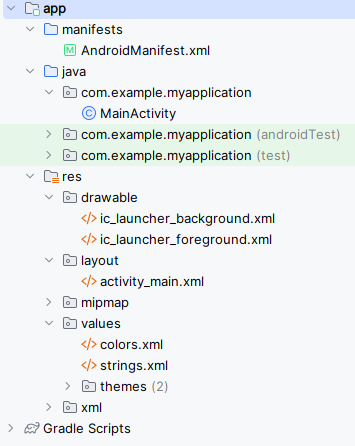
\includegraphics[scale=0.56]{assets/pictures/android_app_struct.png}
  \caption{Основна структура \textit{Android} пројекта}
  \label{pic:android_app_struct}
\end{figure}

Да би се побољшала брзина апликације и смањила потрошња батерије, \textit{Android}-уређаји користе оптимизоване формате за преведени код уместо извршних фајлова језика на коме је код писан. У случају програмског језика \textit{Java}, изворни \textit{Java} код ће се превести у бајткод, а паковање апликације за \textit{Android} у \textit{APK} фајл ће, поред преведеног \textit{Java} кода, садржати библиотеке и ресурсе потребне за рад апликације. \textit{APK} фајл се може извршити на физиком уређају или на виртуелном уређају са \textit{Android}-ом (енг. \textit{Android virtual device, AVD}) који обезбеђује \textit{Android Studio}.

Преведен \textit{Android} код се извршава у извршном \textit{Android} окружењу \textit{ART} (енг. \textit{Android runtime}) директно на процесору уређаја са \textit{Android}-ом обезбеђујући већу уштеду батерије и брже извршавање. Свака апликација се извршава у сопственом процесу чиме се спречава да једна апликација приступи ресурсима друге апликације и уколико нека од апликација престане да ради услед одређене грешке, то неће утицати на друге апликације. На овај начин се доприноси безбедности и сигурности апликација за \textit{Android}. При покретању нове активности апликације, \textit{Android} проверава да ли постоји процес за апликацију којој та активност одговара, ако постоји, користиће њега, у супротном ће направити нови процес. Корисников интерфејс може да ажурира једино главна \textit{Android} нит \cite{AndroidBezOklevanja}.


\section{Животни циклус \textit{Android} активности}


\textit{Android} активности наслеђују класу \texttt{android.app.Activity} чије методе животног циклуса подразумевано користе. Ове методе можемо надјачати (енг. \textit{override}) уколико потребе апликације коју развијамо то захтевају, уз првобитно обавезно позивање методе наткласе. Животни циклус активности се креће из стања \textit{покренута (енг. launched)}, у стање \textit{извршава се (енг. running)} и завршава у стању \textit{уништена (енг. destroyed)}. 

При прављењу активности, позива се њена метода \texttt{onCreate()}. Да бисмо обавестили \textit{Android} који распоред активности треба да користи, ову методу треба надјачати додавањем методе \texttt{setContentView()}. Овде такође додајемо сва подешавања активности које желимо да се одраде у току њеног стварања. Разлог зашто се за прављење активности не користи конструктор, већ метода, је што \textit{Android} пре прављења активности треба да постави окружење за њу. \texttt{onCreate()} мора да се заврши да би се распоред појавио на уређају, стога у овој методи не смемо имати бесконачне петље.

Активност проводи највише времена у стању извршавања и тада је у првом плану на екрану. Активност може бити прекинута наредбом прекида, ако \textit{Android} донесе одлуку да је потребна уштеда простора или да би се поново креирала након промене конфигурације уређаја, попут орјентације или величине екрана. На пример, можда је потребно променити распоред ако је положај екрана уређаја промењен у хоризонталан положај. Ресурси потребни за апликацију могу зависити од конфигурације уређаја, нпр. уколико се промени језик који се користи на телефону, користиће се други скуп ресурса ниски. У случају промене конфигурације уређаја, \textit{Android} ће уништити тренутну активност и поново је направити са ресурсима потребним за нову конфигурацију уређаја. Метод \texttt{onDestroy()} се позива непосредно пре уништења активности. Уколико је потребно, ова метода се може надјачати тако да се ослободе ресурси или обаве друга завршна чишћења. Пре позива \texttt{onDestroy()}, текуће стање активности се може сачувати позивом методе \texttt{onSaveInstanceState()} која као аргумент прима \texttt{Bundle} објекат у коме чува стање активности. Како метода \texttt{onCreate()} такође има овај аргумент, претходно стање активности се може ресетовати када се активност поново буде правила. 

Након методе \texttt{onCreate()}, позива се метода \texttt{onStart()} која обезбеђује да активност постане видљива кориснику и пређе у стање извршавања. Активност може прећи у стање \textit{заустављена (енг. stopped)} ако се у потпуности сакрије другом активношћу и престане да буде видљива кориснику. У овом случају, активност ће и даље постојати у позадини и задржати све информације стања. Овај прелазак обезбеђује метода \texttt{onStop()} која се такође позива и пре методе \texttt{onDestroy()} ако ће активност бити уништена. У овом случају, потребно је позвати методу \texttt{onSaveInstanceState()} пре позива \texttt{onStop()} методе. Метода \texttt{onRestart()} се позива када активност постаје поново видљива након што је била у стању заустављена.

Уколико активност изгуби фокус, тј. престане да буде у првом плану, али је и даље видљива, онда се она налази у стању \textit{паузирана (енг. paused)}. У овом случају, активност и даље ради и задржава све информације о стању. Активност прелази из стања извршавања у ово стање методом \texttt{onPause()}, а враћа се у стање активности методом \texttt{onResume()}. Ова метода се позива и након \texttt{onStart()} методе како би активност прешла у први план. Ако је активност видљива, а никада није у првом плану, онда ће се методе \texttt{onPause()} и \texttt{onResume()} прескочити. Такође, када долази до уништавања активности, метода \texttt{onPause()} ће се позвати пре методе \texttt{onStop()}. 

Целокупан описан процес је представљен на слици \ref{pic:android_activity_lifecycle} \cite{AndroidBezOklevanja}.
Опис израде сложеније апликације за \textit{Android} ће бити приказан у поглављу \ref{chapter:impl-client-app}.

\begin{figure}[h]
  \centering
  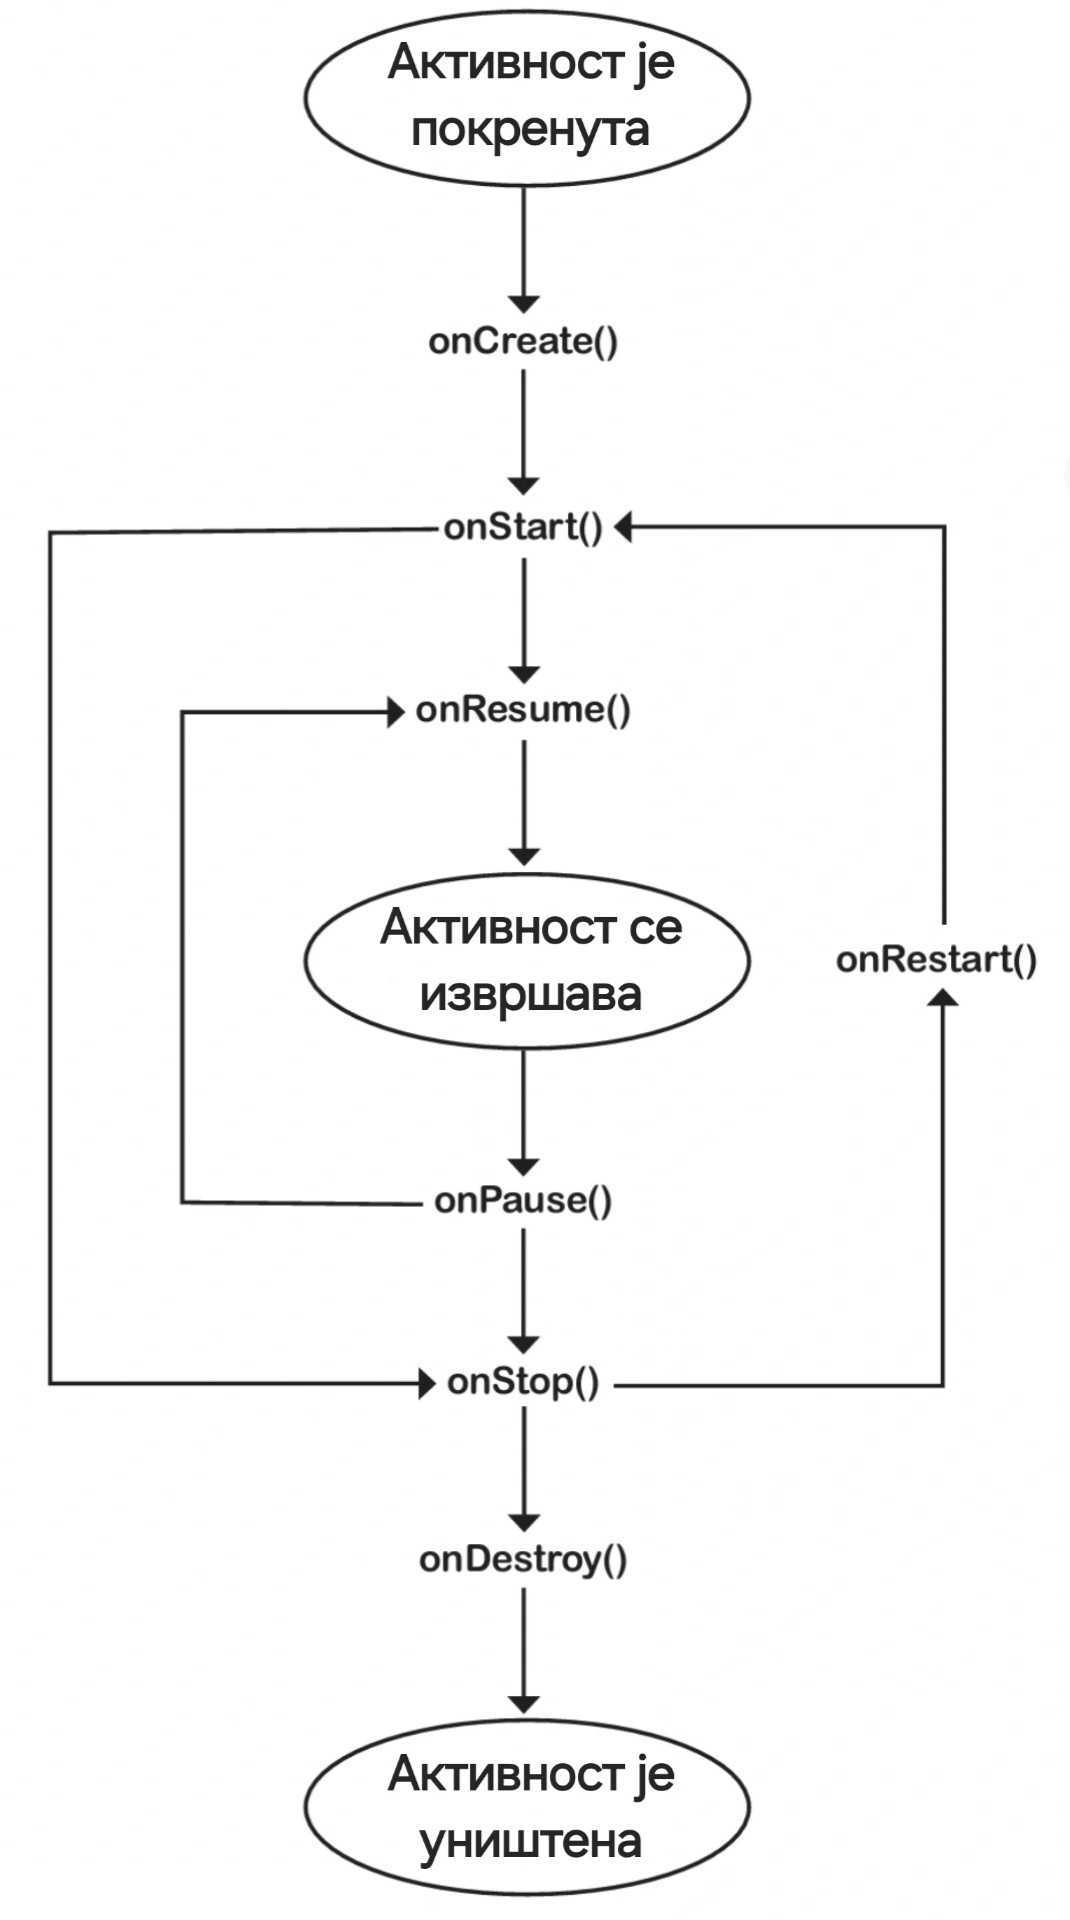
\includegraphics[scale=0.22]{assets/pictures/android_activity_lifecycle.jpg}
  \caption{Животни циклус \textit{Android} активности}
  \label{pic:android_activity_lifecycle}
\end{figure}


\chapter{Оквири \textit{Django} и \textit{Django REST Framework}}\label{chapter:django-theory}

У првим корацима веб развоја, програмери су писали веб странице ручно користећи \textit{HTML}. Уколико би веб сајт требало ажурирати,
то је подразумевало мењање свих \textit{HTML} страница које та измена обухвата. У случају великих сајтова, ажурирање је представљало 
напоран посао који је одузимао доста времена.

Први напредак у односу на овај приступ је направила група инжењера из \textit{Националног центра за суперрачунарске апликације 
(енг. the National Center for Supercomputing Applications, NCSA)} која је креирала \textit{Општи приступни интерфејс 
(енг. Common Gateway Interface, CGI)}, протокол који омогућава веб серверима да динамички генеришу \textit{HTML} странице уз помоћ екстерних програма. 

Међутим, и \textit{CGI} је имао своје недостатке -- CGI скрипте су морале да имају доста поновљеног шаблонског кода, што је усложњавало његово вишеструко искоришћење и отежавало програмерима разумевање пројеката на почетку рада.

У сфери веб програмирања, појављује се програмски језик \textit{PHP} који решава многе наведене проблеме и постаје један од најпопуларнијих алата за креирање динамичких веб сајтова. Његове главне погодности јесу једноставност коришћења, будући да се лако уграђује у \textit{HTML}, и блага крива учења за познаваоце \textit{HTML-а}. Нажалост, ни ово решење није прошло без недостатака, безбедносна заштита коју \textit{PHP} нуди није била на високом нивоу, а лакоћа писања \textit{PHP} кода је лако доводила до несистематичности и дуплирања кода.

Ово је довело до развијања веб оквира нове генерације способних да се изборе са 
већином изазова и амбиција веб програмирања. Овој генерацији припадају оквири \textit{Ruby
on Rails} и \textit{Django}. \textit{Django} омогућава развијање комплексних и динамичких веб сајтова за кратко време захваљујући апстракцији високог нивоа уобичајених шаблона веб развоја и јасним упутствима и методама за решавање учесталих програмерских задатака. На тај начин, програмери се могу фокусирати на кључну логику, док ће се \textit{Django} побринути за све рутинске задатке \cite{GuideToDjango}.

\section{Основни концепти}

\textit{Django} \cite{GuideToDjango, DjangoforAPIs} је веб оквир програмског језика \textit{Python} који је први пут објављен 2005. године. Заснива се на филозофији дизајна програмских алата која подразумева да се њиховом инсталацијом добија богати скуп уграђених функционалности које омогућавају корисницима да одмах почну са радом. \textit{Django} настоји да очува овај принцип пружајући корисницима стандардну библиотеку са разним додацима (енг. \textit{add-ons}) за најчешће задатке веб развоја. Његова главна предност је управљање свим захтевнијим деловима израде веб сајта као што је аутентификација, повезивање са базом, безбедност итд.

\textit{Django} такође следи принцип \textit{''без понављивања'' (енг. ''Don't Repeat Yourself'', DRY)}. Ово је основни принцип програмског развоја који промовише избегавање дуплирања кода. Како би подстакао програмере да пишу код који није редудантан, \textit{Django} има неколико уграђених механизама попут система шаблона, наслеђивања модела, међуслојног оквира (енг. \textit{middleware}) који омогућава дефинисање поновно употребивих компоненти за обрађивање \textit{HTTP} захтева и одговора и др.1425

Овај оквир је отвореног кода и доступан је на репозиторијуму за додатке за 
програмски језик \textit{Python}, \textit{\href{https://pypi.org}{Python Package Index (PyPI)}}\footnote{https://pypi.org} као и сви његови додатни пакети који су на располагању програмерима. У наставку су детаљније описане главне карактеристике овог оквира.


\subsection{Постављање и конфигурација \textit{Django} пројекта}

Нови \textit{Django} пројекат се креира командом

\lstset{
  language=Python,
  basicstyle=\ttfamily,
  keywordstyle=\color{blue},
  frame=single
}
\begin{lstlisting}
    django-admin startproject $project_name $storing_dir
\end{lstlisting}


Први аргумент команде \texttt{startproject} је име које желимо да дамо новом пројекту. Други аргумент дефинише директоријум који ће садржати основне фајлове и структуру пројекта. Уколико га не дефинишемо, додатни директоријум са именом пројекта ће се креирати у тренутном радном директоријуму.

У случају да корисник позове претходну команду на следећи начин:
\lstset{
  language=Python,
  basicstyle=\ttfamily,
  keywordstyle=\color{blue},
  frame=single
}
\begin{lstlisting}
    django-admin startproject django_project_name .
\end{lstlisting}

\noindent \textit{Django} ће у тренутном радном директоријуму креирати наредну структуру пројекта:
\lstset{
  language=Python,
  basicstyle=\ttfamily,
  keywordstyle=\color{blue},
  frame=single
}
\begin{lstlisting}
|-- django_project_name
|    |-- __init__.py
|    |-- asgi.py
|    |-- settings.py
|    |-- urls.py
|    |-- wsgi.py
|-- manage.py
\end{lstlisting}

Од највеће важности за стандардне пројекте су наредни фајлови:
\begin{itemize}[--]
    \item \texttt{settings.py} -- контролише општа подешавања \textit{Django} пројекта,
    \item \texttt{urls.py} -- служи за рутирање \textit{HTTP} захтева и
    \item \texttt{manage.py} --  скрипта намењена за извршавање различитих \textit{Django} команди.
\end{itemize}

Коришћењем \texttt{manage.py} скрипте, \textit{Django} пројекат се покреће на локалном веб серверу на следећи начин:
\begin{lstlisting}
    python manage.py runserver
\end{lstlisting}

\noindentДа би се потврдило да је пројекат успешно инсталиран, потребно је отворити адресу \url{http://127.0.0.1:8000} у веб прегледачу. У случају успешног покретања, корисник ће добити страницу са изгледом приказаним на слици \ref{pic:django_initial_run}.

\begin{figure}[h]
  \centering
  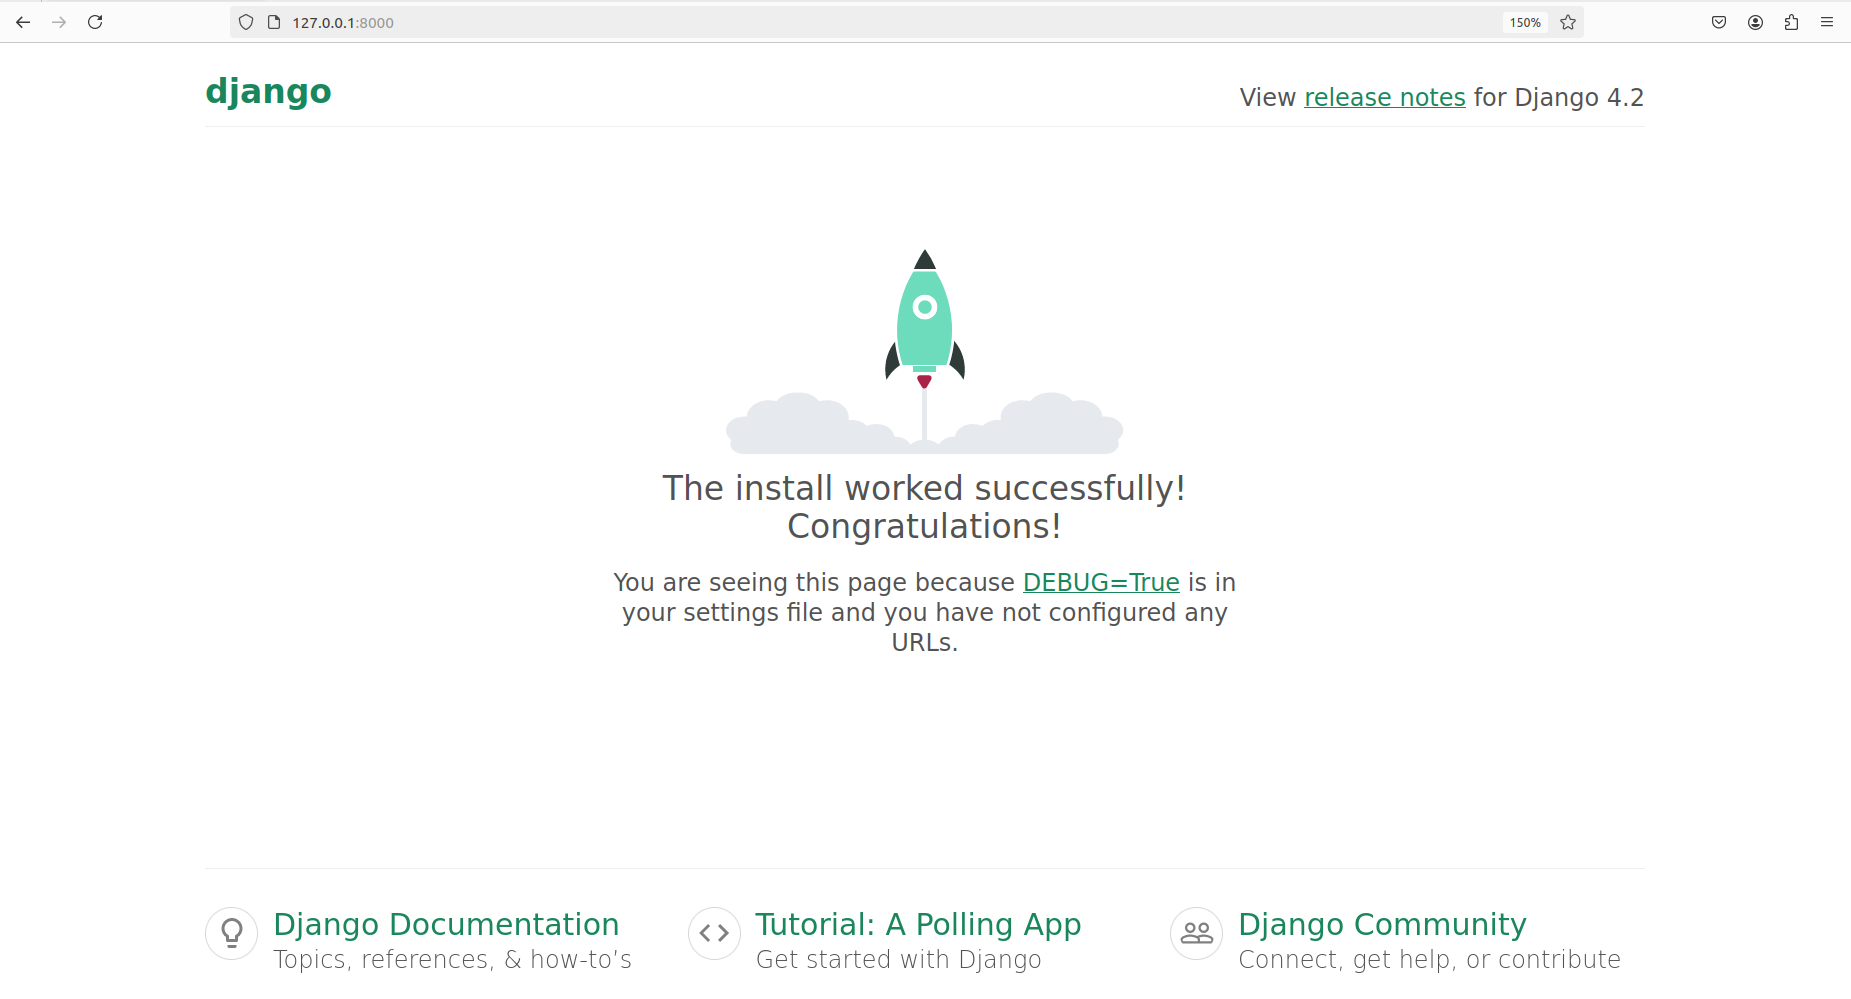
\includegraphics[scale=0.22]{assets/pictures/django_initial_project_run.png}
  \caption{Изглед веб странице иницијално постављеног \textit{Django} пројекта}
  \label{pic:django_initial_run}
\end{figure}

Традиционалан \textit{Django} веб сајт се састоји од једног пројекта са више апликација, где свака апликација представља одвојену функционалност.
За прављење нове апликације унутар пројекта се користи наредна команда:

\lstset{
  language=Python,
  basicstyle=\ttfamily,
  keywordstyle=\color{blue},
  frame=single
}
\begin{lstlisting}
    python manage.py startapp $app_name
\end{lstlisting}
где је \texttt{\$app\_name} име апликације која се креира. У случају конкретног позива
\lstset{
  language=Python,
  basicstyle=\ttfamily,
  keywordstyle=\color{blue},
  frame=single
}
\begin{lstlisting}
    python manage.py startapp new_app
\end{lstlisting}
креираће се директоријум \texttt{new\_app} са следећом структуром:
\lstset{
  language=Python,
  basicstyle=\ttfamily,
  keywordstyle=\color{blue},
  frame=single
}
\begin{lstlisting}
|-- new_app
|    |-- __init__.py
|    |-- admin.py
|    |-- apps.py
|    |-- migrations
|         |-- __init__.py
|    |-- models.py
|    |-- tests.py
|    |-- views.py
|-- django_project (prethodno kreiran)
\end{lstlisting}

где су:
\begin{itemize}[--]
    \item \texttt{admin.py} -- конфигурациони фајл за уграђену апликацију \textit{Django Admin},
    \item \texttt{apps.py} -- конфигурациони фајл за новокреирану апликацију,
    \item \texttt{migrations/} -- директоријум за чување миграционих фајлова за промене у бази података,
    \item \texttt{models.py} -- модул за дефинисање модела базе података,
    \item \texttt{tests.py} -- модул за тестове новокреиране апликације, а
    \item \texttt{views.py} -- модул за обраду логике \textit{HTTP} захтева и одговора.
\end{itemize}

Додатно, потребно је креирати фајл \texttt{urls.py} за рутирање на нивоу апликације.


Да би \textit{Django} препознао и учитао апликацију, неопходно је да се региструје у конфигурацији \texttt{INSTALLED\_APPS} у конфигурационом фајлу \\
\texttt{django\_project/settings.py}: \\

\lstset{
  language=Python,
  basicstyle=\ttfamily,
  keywordstyle=\color{blue},
  frame=single
}
\begin{lstlisting}
# django_project/settings.py

INSTALLED_APPS = [
    ...
    "new_app.apps.NewAppConfig"
    ...
]
\end{lstlisting}

\subsection{\textit{MVT} архитектура}

Архитектура оквира \textit{Django} се темељи на обрасцу \textit{Модел-Поглед-Шаблон (енг. Model-View-Template, MVT)} који омогућава јасно раздвајање између 
управљања подацима (модели), пословне логике (погледи) и презентације (шаблони). За моделе се користи фајл \texttt{models.py}, за погледе  \texttt{views.py}, а за шаблоне директоријум \texttt{templates/}. У наставку су детаљније описане компоненте ове архитектуре.

\subsubsection{Mодели}

Модели представљају апстракцију базе података и омогућавају рад са подацима на високом нивоу кроз интеракцију са базом података, без директног коришћења \textit{SQL} упита. Модели дефинишу структуру табела у бази података кроз \textit{Python} класе. Атрибути класе представљу колоне у табели, док инстанце класе представљу редове, тј. записе. Атрибути класе модела, познатији као \textit{поља (Fields)}, дефинишу тип и карактеристике података у бази. На располагању су разноврсни типова поља, укључујући текстуални \texttt{(CharField)}, целобројни \texttt{(IntegerField)}, датумски \texttt{(DateField)}, тип података за електронску пошту \texttt{(EmailField)}, \textit{URL} адресе \texttt{(URLField)} и др. Списак свих доступних типова као и њихови детаљни описи су доступни у званичној \textit{Django} документацији о типовима поља\footnote{https://docs.djangoproject.com/en/5.0/ref/models/fields/}.

Рад са базом података без коришћења \textit{SQL} упита је омогућен захваљујући \textit{Објектно-Релационом мапирању (енг. Object-Relational Mapping, ORM)} које прави мост између објектно-орјентисаног програмирања и релационих база података. У оквиру \textit{Django}, \textit{ORM} обезбеђује једноставно и ефикасно извођење операција креирања, читања, ажурирања и брисања \textit{(енг. CRUD - create, read, update, delete)} над базом података.

На пример, за креирање табеле са ауторима која садржи колоне са јединственим идентификатором, именом, презименом и датумом рођења аутора, потребно је креирати класу са наведеним атрибутима у фајлу \texttt{models.py}.

\lstset{
  language=Python,
  basicstyle=\ttfamily,
  keywordstyle=\color{blue},
  frame=single
}
\begin{lstlisting}
# django_project/models.py

from django.db import models

class Author(models.Model):
    id = models.PositiveBigIntegerField(primary_key=True)
    first_name = models.CharField()
    last_name = models.CharField()
    birth_date = models.DateField()
\end{lstlisting}


Креирање новог уноса у табелу се ради инстанцирањем направљене класе и коришћењем методе \texttt{save()} које је неопходна за ажурирање базе података. \\

\lstset{
  language=Python,
  basicstyle=\ttfamily,
  keywordstyle=\color{blue},
  frame=single
}
\begin{lstlisting}
author = Author(id=1, 
                first_name="John", 
                last_name="Doe", 
                birth_date="1980-01-01")
author.save()
\end{lstlisting}

У наредном коду су приказани примери читања свих аутора и аутора са идентификатором вредности \texttt{1} из базе.
\lstset{
  language=Python,
  basicstyle=\ttfamily,
  keywordstyle=\color{blue},
  frame=single
}
\begin{lstlisting}
authors = Author.objects.all()
author = Author.objects.get(id=1)
\end{lstlisting}

Наредни код мења презиме аутора са идентификатором вредности \texttt{1}.
\lstset{
  language=Python,
  basicstyle=\ttfamily,
  keywordstyle=\color{blue},
  frame=single
}
\begin{lstlisting}
author = Author.objects.get(id=1)
author.last_name = "Smith"
author.save()
\end{lstlisting}

Брисање записа из базе се ради коришћењем методе \texttt{delete()} над конкретном инстанцом одговарајуће класе.
\lstset{
  language=Python,
  basicstyle=\ttfamily,
  keywordstyle=\color{blue},
  frame=single
}
\begin{lstlisting}
author = Author.objects.get(id=1)
author.delete()
\end{lstlisting}

\vspace{0.5cm}
Једна од важних могућности модела је \textbf{валидација података}. \textit{Django} пружа уграђене механизме за валидацију кроз поља модела. На пример, \texttt{CharField} може имати ограничење за максималну дужину текста:

\lstset{
  language=Python,
  basicstyle=\ttfamily,
  keywordstyle=\color{blue},
  frame=single
}
\begin{lstlisting}
first_name = models.CharField(max_length=30)
last_name = models.CharField(max_length=30)
\end{lstlisting}

Такође, могуће је дефинисати методе за валидацију унутар модела. У наредном примеру је додато ограничење да датум рођења аутора мора бити мањи од тренутног.

\lstset{
  language=Python,
  basicstyle=\ttfamily,
  keywordstyle=\color{blue},
  frame=single,
  showstringspaces=false
}
\begin{lstlisting}
# django_project/author/models.py

from django.db import models
from django.core.exceptions import ValidationError
from datetime import datetime

class Author(models.Model):
    id = models.PositiveBigIntegerField(primary_key=True)
    first_name = models.CharField(max_length=30)
    last_name = models.CharField(max_length=30)
    birth_date = models.DateField()

    def check_birth_date(self):
        if self.birth_date >= datetime.date.today():
            raise ValidationError("Birth date cannot be 
                                   future date.")
\end{lstlisting}

\vspace{0.5cm}
\textbf{Миграције} у \textit{Django}-у \cite{django_doc_migrations} су механизам за примењивање извршених промена насталих у моделима у бази података. Овај процес је веома важан за одржавање конзистентности и интегритета података у апликацији. Свака промена у моделима у \textit{Django} апликацији захтева креирање миграције. Миграције треба правити приликом додавања новог модела, измена постојећег или брисања модела. \textit{Django} пружа неколико команди које олакшавају рад са миграцијама:

\begin{itemize}[--]
    \item \texttt{migrate} -- за примењивање и повлачење миграције у базу,
    \item \texttt{makemigrations} -- креира нове миграције на основу промена у моделима,
    \item \texttt{sqlmigrate} -- приказује \textit{SQL} упите који ће бити извршени за одређену миграцију и
    \item \texttt{showmigrations} -- приказује листу миграција и њихов статус (да ли су примењене или нису).
\end{itemize}

Наведене команде се покрећу над фајлом \texttt{manage.py}. Прво је потребно направити миграциони фајл са командом \texttt{makemigrations},
\lstset{
  language=Python,
  basicstyle=\ttfamily,
  keywordstyle=\color{blue},
  frame=single
}
\begin{lstlisting}
    python manage.py makemigrations
\end{lstlisting}
а затим применити све непримењене миграције командом \texttt{migrate} која ће синхронизовати базу података са тренутним стањем модела.
\lstset{
  language=Python,
  basicstyle=\ttfamily,
  keywordstyle=\color{blue},
  frame=single
}
\begin{lstlisting}
    python manage.py migrate
\end{lstlisting}

\subsubsection{Погледи}\label{django:url_routing}

\textit{Функција погледа (енг. view function)} \cite{django_doc_views} је \textit{Python} функција која као улазну вредност добија веб захтев, а на излазу враћа веб одговор. Одговор може бити садржај \textit{HTML} странице, преусмеравање, грешка, документ и сл. 

Како би се одговор специфичне поглед функције приказао, потребно је конфигурисати фајл \texttt{urls.py} који је задужен за рутирање у \textit{Django} апликацијама. Овај фајл дефинише \textit{URL} руте и повезује их са одговарајућим поглед функцијама. Када корисник пошаље захтев на одређену \textit{URL} адресу, \textit{Django} на основу овог фајла проналази одговарајућу поглед функцију која ће обрадити захтев и вратити одговор. За дефинисање рутирања, обично се користи функција \texttt{path()} која као први аргумент узима назив \textit{URL} шаблона у облику ниске, други аргумент представља одговарајућу поглед функцију, док опционо може имати трећи аргумент за именовање рута које се може користити у шаблонима.

\shorthandoff{"}
Наредни пример приказује све ауторе из базе података на рути \texttt{"authors/"} користећи шаблоне који су објашњени у наставку.
\shorthandoff{"}

\lstset{
  language=Python,
  basicstyle=\ttfamily,
  keywordstyle=\color{blue},
  frame=single,
  showstringspaces=false
}
\begin{lstlisting}
# django_project/author/urls.py

from django.urls import path
from .views import home_view, authors_view

urlpatterns = [
    path('authors/', authors_view, name='authors'),
]
\end{lstlisting}


\lstset{
  language=Python,
  basicstyle=\ttfamily,
  keywordstyle=\color{blue},
  frame=single,
  showstringspaces=false
}
\begin{lstlisting}
# django_project/author/views.py

from django.shortcuts import render
from .models import Author

def authors_view(request):
    authors = Author.objects.all()
    return render(request, 'authors.html', 
                  {'authors': authors})
\end{lstlisting}

\subsubsection{Шаблони}

Шаблони у \textit{Django}-у представљају концепт који омогућава програмерима да одвоје презентациони од логичког слоја апликације, чиме се постиже боља организација и одржавање пројекта. \textit{Језик Django шаблона (енг. Django template language, DTL)} \cite{django_doc_dtl} омогућава укључивање динамичких елемената у статичке \textit{HTML} шаблоне. Ови елементи се називају \textit{тагови} и понашају се слично као програмске контролне структуре (попут наредби \texttt{if}, \texttt{for}...), али се не извршавају као \textit{Python} код. Стога, није могуће навести обичан \textit{Python} код, већ само оно што \textit{DTL} подржава. Шаблон садржи променљиве које се евалуирају у вредности и тагове који контролишу логику. Тагови се увек наводе у формату \texttt{\{\% tag \%\}}. За апликацију \texttt{author}, \textit{Django} ће подразумевано тражити шаблон на путањи \texttt{author/templates/}. 

Kонвенција је да се унутар директоријума \texttt{templates} креира поддиректоријум са истим именом као апликација у коме ће се сместити шаблони. У наредном примеру је приказан шаблон за пролазак кроз све ауторе у бази и њихово приказивање.

\lstset{
  language=HTML,
  basicstyle=\ttfamily,
  keywordstyle=\color{blue},
  frame=single
}
\begin{lstlisting}
<!-- author/templates/author/author_list.html -->

<h1>All authors</h1>

<ul>
    <li>Id: {{ author.id }}</li>
    <li>Name: {{ author.first_name }}</li>
    <li>Surname: {{ author.last_name }}</li>
    <li>Birth date: {{ author.birth_day }}</li>
</ul>

\end{lstlisting}


\section{\textit{Django REST Framework}}

Скуп протокола и инструкција које одређују како ће две програмске компоненте остварити директну комуникацију представља \textit{програмски интерфејс апликације (енг. Application Programming Interface, API)}. Када је \textit{Django} настао, већина веб сајтова је била заснована 
на апикацијама са монолитном архитектуром у којима су презентациони слој, логички слој као и база података интегрисани унутар једне самосталне целине.
Данас се често користи \textit{приступ који даје приоритет API-ју (енг. API-first approach)} где се апликација раздваја на две компоненте, клијентску (енг. \textit{frontend}) и серверску (енг. \textit{backend}) апликацију, које комуницирају путем \textit{API}-ја. Клијентска апликација је задужена за презентациони слој и прослеђивање захтева серверској апликацији која управља логичким слојем и базом података. Један \textit{API} може истовремено подржати више различитих клијентских апликација развијених у различитим програмским језицима и оквирима. Такође, уколико се клијентска апликација ажурира новијим верзијама алата, \textit{API} може остати исти.

Код веб \textit{API}-ја, преовладава архитектурни образац \textit{REST (REpresentational State Transfer)} \cite{restful_web_apis} чији је кључни појам ресурс. Ресурс може бити било који ентитет довољно битан да може бити референциран. Сваки ресурс мора имати свој \textit{URL}. Да би \textit{API} био \textit{RESTful API}, неопходно је да испуњава наредна три својства:
\begin{enumerate}
    \item Да нема стања (енг. \textit{stateless}) као и \textit{HTTP} протокол над којим је \textit{RESTful API} изграђен\footnote{Сваки пар \textit{HTTP} захтев -> \textit{HTTP} одговор је независан од претходног и не постоји меморија која чува стање између захтева}
    \item Подржава уобичајене \textit{HTTP} методе (\textit{GET}, \textit{POST}, \textit{PUT}, \textit{DELETE}, итд.)\footnote{Метода \textit{HTTP GET} се користи за добијање ресурса, \textit{POST} за креирање нових ресурса, \textit{PUT} за ажурирање постојећих ресурса, \textit{DELETE} за брисање ресурса, итд.}
    \item Враћа податке у \textit{JSON} или \textit{XML} формату
\end{enumerate}

Оквир \textit{Django REST Framework (DRF)} омогућава програмерима да постојећи \textit{Django} пројекат трансформишу у веб \textit{API}. Главни недостатак приступа који даје приоритет \textit{API}-ју је што захтева више конфигурације него традиционална \textit{Django} апликација. Међутим, \textit{DRF} поседује механизме који олакшавају имплементацију веб \textit{API}-ја. Да би се постојећа традиционална \textit{Django} апликација трансформисала у веб \textit{API}, потребно је ажурирати фајл \texttt{urls.py}, додати \textit{DRF} погледе и креирати серијализатор (енг. \textit{serializer}). Серијализатор претвара комплексне податке (нпр. \textit{Django} моделе) у формате за слање серијализованих података које је једноставно користити, најчешће у \textit{JSON} или \textit{XML} формат и прима и валидира податке у овим форматима пре чувања у бази.

Да би се \textit{DRF} користио у пројекту, потребно га је инсталирати користећи \textit{PyPI} и регистровати у конфигурацији \texttt{INSTALLED\_APPS} у конфигурационом фајлу \texttt{django\_project/settings.py}:

\lstset{
  language=Python,
  basicstyle=\ttfamily,
  keywordstyle=\color{blue},
  frame=single
}
\begin{lstlisting}
# django_project/settings.py

INSTALLED_APPS = [
    ...
    "rest_framework",
    ...
]
\end{lstlisting}


\shorthandoff{"}
Уколико се сва \textit{API} логика смешта на рути \texttt{"api/"}, потребно је направити апликацију \texttt{api} и ажурирати фајл \texttt{django\_project/urls.py} у складу са претходно наведеним објашњењима за традиционалну \textit{Django} апликацију. Уколико желимо да направимо \textit{API} за приказ свих аутора у \textit{JSON} формату, \textit{URL} фајл за апликацију \texttt{apis/urls.py} је потребно ажурирати тако да на рути \texttt{""} приказује поглед 
\shorthandoff{"}
\texttt{AuthorAPIView} који ћемо креирати.

\lstset{
  language=Python,
  basicstyle=\ttfamily,
  keywordstyle=\color{blue},
  frame=single
}
\begin{lstlisting}
# apis/urls.py

from django.urls import path

from .views import AuthorAPIView

urlpatterns = [
    path("", AuthorAPIView.as_view(), name="author_list"),
]
\end{lstlisting}

Погледи \textit{DRF}-а се разликују од погледа традиционалне \textit{Django} апликације у формату података које враћају, традиционална \textit{Django} апликација ће враћати садржај \textit{HTML} странице, док \textit{DRF} враћа серијализоване податке у медијским форматима попут формата \textit{JSON}, \textit{XML}, итд. Наредни код користи генеричку класу \texttt{ListAPIView} за читање свих инстанци аутора. Потребно је дефинисати атрибуте \texttt{queryset} и \texttt{serializer\_class} ове класе коју ће наша класа \texttt{AuthorSerializer} која је наслеђује користити. Атрибуту \texttt{queryset} додељујемо инстанце свих аутора, док класу за серијализатор, \texttt{serializer\_class}, постављамо на \texttt{AuthorSerializer} коју ћемо дефинисати у модулу за серијализатор.

\lstset{
  language=Python,
  basicstyle=\ttfamily,
  keywordstyle=\color{blue},
  frame=single
}
\begin{lstlisting}
# apis/views.py

from rest_framework import generics
from books.models import Author
from .serializers import AuthorSerializer

class AuthorAPIView(generics.ListAPIView):
    queryset = Author.objects.all()
    serializer_class = AuthorSerializer
\end{lstlisting}

Приликом дефинисања серијализатора, потребно је обезбедити модел базе који ће се читати и поља која желимо да прикажемо.

\lstset{
  language=Python,
  basicstyle=\ttfamily,
  keywordstyle=\color{blue},
  frame=single
}
\begin{lstlisting}
# apis/serializers.py

from rest_framework import serializers
from books.models import Author

class AuthorSerializer(serializers.ModelSerializer):
    class Meta:
        model = Author
        fields = ("id", 
                  "first_name", 
                  "last_name", 
                  "birth_date")
\end{lstlisting}

\shorthandoff{"}
Уколико су претходни кораци успешно одрађени, након покретања \textit{Django} пројекта на локалном веб серверу, на рути \texttt{"api/"} ћемо моћи да видимо списак свих аутора из базе података у \textit{JSON} формату.
\shorthandoff{"}
\vspace{0.7cm}

Овим смо обухватили основне концепте и функционалности оквира \textit{Django} и \textit{Django REST Framework}, показујући како се користе за развој робусних и скалабилних веб апликација. У поглављу \ref{chapter:impl-server-app} ћемо приказати његову конкретну употребу на сложенијој апликацији.


\chapter{Серверска страна апликације \textit{Train Wiser}}\label{chapter:impl-server-app}

Употреба технологија описаних у претходним поглављима представљена је у практичном делу рада - креираној апликацији \textit{Train Wiser} \cite{train_wiser_implementation}. Апликација пружа статистку и асистенциjу за тренирање и напредак вежбача на основу корисничких података увезених са апликације \textit{Strava} путем њеног јавног програмског интерфејса и на основу резултата трка одржаних у Републици Србији. 
Апликација \textit{Train Wiser} је намењена тркачима који желе да детаљније прате своје перформансе и да унапреде резултате.

За архитектуралну организацију апликације одабран је модел клијент-сервер. У овом моделу, клијентска апликација (енг. \textit{frontend}) је задужена за комуникацију са корисником и прослеђивање захтева серверској апликацији (енг. \textit{backend}) која је задужена за унутрашњу логику. У овом поглављу су представљене кључне тачке и додатне технологије коришћене у изради серверског дела апликације, њена архитектура и јавни интерфејс за програмирање апликација.


\section{Кључни аспекти при развоју апликације}

За израду серверског дела апликације, коришћен је програмски језик \textit{Python} уз оквире \textit{Scrapy},
\textit{Django} и \textit{Django REST Framework}. У наставку су кроз кључне тачке при развоју апликације издвојени описи неких од додатно употребљених технологија.

\subsection{Aутентификација и ауторизација} \label{subsec:authorization_and_authentication}

Аутентификација и ауторизација представљају кључне концепте безбедносности система.

Аутентификација је процес доказивања идентитета одређених ентитета, корисника или других система (у даљем тексту - корисника), и утврђивања да ли је тим корисницима дозвољен приступ систему. Доказивање идентитета најчешће подразумева прилагање корисничког имена и лозинке, а додатно се могу тражити и биометријски подаци и/или аутентификацијски токени.
Ауторизација, с друге стране, долази након аутентификације, и подразумева додељивање права и привилегија аутентификованом кориснику. На овај начин се одређује којим ресурсима система корисник има дозволу да приступи, као и скуп акција које може извршити. 

У савременим веб апликацијама, често се јавља потреба да једна апликација приступа ресурсима друге апликације у име корисника. Овај концепт је важан у контексту интеграције различитих услуга и обезбеђивања доброг корисничког искуства. На пример, апликација може имати опцију за предлагање контакта на основу пратилаца са одређене друштвене мреже корисника, и да за то тражи од корисника да се пријави на ту друштевену мрежу.

Уколико би апликација добила корисничке податке за аутентификацију како би се аутентификовала на друштвеној мрежи, она поред приступа листи пратилаца добија потпун приступ корисничком налогу. Такође, апликација би имала могућност да сачува корисничке податке за аутентификацију за друштвену мрежу, као и да то уради на небезбедан начин. У случају да се апликација компромитује, подаци за аутентификацију за друштвену мрежу би такође били компромитовани. Наведене проблеме оваквог приступа настоји да реши протокол \textit{OAuth 2.0}.

\textit{OAuth 2.0} омогућава апликацијама да добију ограничени приступ корисничким ресурсима на спољним сервисима без прослеђивања података за аутентификацију за пријављивање апликацији, истовремено задржавајући висок ниво безбедности. Апликација ће приступати ресурсима у складу са датим дозволама од стране корисника, чиме се повећава контрола над приватним подацима. \\ 
Два најчешћа случаја употребе су:

1. Аутентификовање корисника на основу налога са спољног сервиса
\begin{itemize}[--]
    \item Овај принцип се зове \textit{федеративни идентитет (енг. federated identity)}. 
    \item На пример, \textit{Instagram} дозвољава корисницима да се пријаве преко \textit{Fa\-ce\-book} налога.
\end{itemize}

2. Пружање дозвола апликацији да приступа ресурсима спољног сервиса у одсуству корисника
\begin{itemize}[--]
    \item Овај принцип се зове \textit{делегирање ауторизације (енг. delegated authority)}. 
    \item На пример, \textit{Instagram} приступа сликама са \textit{Facebook} налога без посредништва корисника.
\end{itemize}


\noindentПринцип рада протокола се заснива на следећим корацима:
\begin{enumerate}
    \item Регистрација апликације
    \item Добијање приступног токена
    \item Преузимање захтеваних ресурса посредством приступног токена
    \item Коришћење токена за обнову приступног токена
\end{enumerate}

\subsubsection*{Регистрација апликације}

Регистрација апликације представља процес који је потребно извршити једанпут како би се успоставила интеграција, односно веза од поверења, између апликације и спољног сервиса. Исход овог процеса је да су апликацији доступни наредни параметри:

\begin{itemize}[--]
    \item \textit{Клијентски идентификатор (енг. client ID)} -- јединствени идентификатор на нивоу спољног сервиса који представља апликацију која жели да се региструје; добија се од спољног сервиса или се дефинише од стране власника апликације 
    \item \textit{Клијентски тајни кључ (енг. client secret)} -- тајни кључ који се увек добија од спољног сервиса. Овај кључ, заједно са клијентским идентификатором, представља податке за аутентификацију апликације који се прилажу спољном сервису како би се обавила аутентификација апликације пре процеса делегирања ауторизације
    \item \textit{Веб адреса за преусмерење одговора од стране спољног сервиса (енг. re\-di\-rec\-tion endpoint)} -- веб адреса на коју спољни сервис шаље одговоре апликацији који обично представљају токене или грешке. Ову веб адресу у највећем броју случајева обезбеђује власник апликације
    \item \textit{Веб адреса ауторизације (енг. authorization endpoint)} -- веб адреса коју ће клијентска апликација користити да иницира процес ауторизације, одређена је од стране спољног сервиса
    \item \textit{Веб адреса за токене (енг. token endpoint)} -- веб адреса обезбеђена од стране спољног сервиса коју ће апликација користити да иницира процес размене токена
\end{itemize}

\subsubsection*{Добијање приступног токена}


Након успешне регистрације, спољни сервис ће aпликацији доделити \textit{приступни токен (енг. access token)}. Приступни токен обезбеђује приступ заштићеним дигиталним ресурсима, ограничавајући друге начине приступа и тиме побољшавајући сигурност.
Овај токен има свој опсег и време трајања. Опсег представља скуп заштићених ресурса 
којима се може приступити, док време трајања представља време након чијег истицања ће присуп са датим токеном постати невалидан.

Уколико спољни сервис подржава обнављављање приступног токена коришћењем 
\textit{токена за обнову (енг. refresh token)}, овај токен ће бити додатно достављен уз приступни токен. Токен за обнову има дуже време трајања од приступног токена и служи за добијање новог приступног токена када постојећи истекне.


\subsubsection*{Преузимање захтеваних ресурса посредством приступног токена}

Након што се корисник аутентификује на спољни сервис на који га је преусмерила апликација и прихвати захтев за ауторизацију,
апликација ће добити приступ оним ресурсима којима је корисник одобрио приступ. Захтев за добијање ресурса треба да садржи приступни токен. 
Приступ захтеваним ресурсима се може радити све док приступни токен не истекне или буде поништен.

\subsubsection*{Коришћење токена за обнову приступног токена}

Након што приступни токен истекне, апликација има опцију да испочетка понови процес аутентификације, што може захтевати да се корисник поново пријави или да користи токен за обнову приступног токена за шта није потребно учешће корисника. У другом случају се нови приступни токен добија кроз захтев за обнову приступног токена уз слање токена за обнову. \\

У претходном процесу разликујемо апликације од поверења и апликације које нису од поверења у зависности да ли 
апликација има могућност да сигурно чува и преноси информације. Апликације засноване на веб прегледачу код којих се све информације чувају у самом прегледачу (нпр. \textit{HTML} и \textit{JavaScript} апликације) као и \textit{Flash} апликације које не захтевају дуготрајан приступ корисничким подацима јесу неке од примера апликација које нису од поверења. Пример апликације од поверења би била апликација која има клијентски и серверски део уз базу података, где је серверски део задужен за безбедно руковање и чување података.

Клијентски тајни кључ, приступни токен и токен за обнову се добијају једино у случају апликације од поверења. 
У контексту апликације која није од поверења, процес добијања захтеваних ресурса је поједностављен. У овом случају, 
сваки пут када апликација има потребу да користи ресурсе спољног сервиса, преусмериће корисника на одобрење 
ауторизације апликације са спољним сервисом. Након што корисник одобри ауторизацију, апликација добија кључ 
од спољног сервиса који ће користити у захтеву за приступ жељеним ресурсима. Спољни сервис ће у случају успешне
валидације кључа проследити апликацији тражене ресурсе \cite{mastering_oauth2}.

Апликација \textit{Strava} користи \textit{OAuth 2.0} \cite{strava_api_oauth2} за аутенификацију са \textit{V3 API}-ем, 
јавним интерфејсом ове апликације који даје могућност програмерима да приступе подацима ове апликације. Апликација \textit{Train Wiser} је преко овог протокола увезана са апликацијом \textit{Strava} како би имала приступ свим активностима корисника који одобре ауторизацију. 


\subsection{Формирање скупа података са активностима корисника}\label{subsec:activities_dataset}

У тренутку када нови корисник одобри ауторизацију са апликацијом \textit{Strava} преко апликације \textit{Train Wiser}, апликација \textit{Train Wiser} ће екстраховати све његове релевантне претходне активности и сместити их у табелу \texttt{StravaActivity} у бази података. Информације о новим активностима корисника се уписују у ову табелу након што их корисних отпреми на апликацији \textit{Strava}.

Будући да \textit{Strava API} допушта максимално 200 упита на сваких 15 минута са највише 2000 упита у дану, допуњавање базе претходним активностима корисника је одрађено коришћењем библиотеке оквира \textit{Django} за планирање задатака, \textit{django-crontab}.
Овај механизам аутоматизације заједно са појмом \textit{мрежних кука (енг. webhooks)} које су коришћене за аутоматско прикупљање нових активности корисника су детаљније описани у наставку.

\subsubsection{Django библиотека \textit{django-crontab}}

\textit{Cron} процес, подразумевано доступан на \textit{Unix} и \textit{Linux} системима, омогућава аутоматизацију извршавања \texttt{shell} команди у одређено време, елиминишући потребу за ручним покретањем. \textit{Cron} се ослања на конфигурациону датотеку \textit{crontab} (скраћено од \texttt{''cron table''}) у којој је у сваком реду уписано време извршавања и, у виду \texttt{shell} команде, посао који је потребно извршити. Ова датотека се од стране \textit{Cron} процеса проверава у сваком минуту, и на основу њених уноса се извршавају доспели послови \cite{linux_pocket_guide}. Један ред ове датотеке представља један \textit{Cron-посао (енг. cronjob)} \cite{cronjob}.
Синтакса за навођење \textit{Cron} послова у \texttt{crontab} датотеци је приказана на слици \ref{pic:crontab_syntax} \cite{linux_pocket_guide}.

\begin{figure}[h]
  \centering
  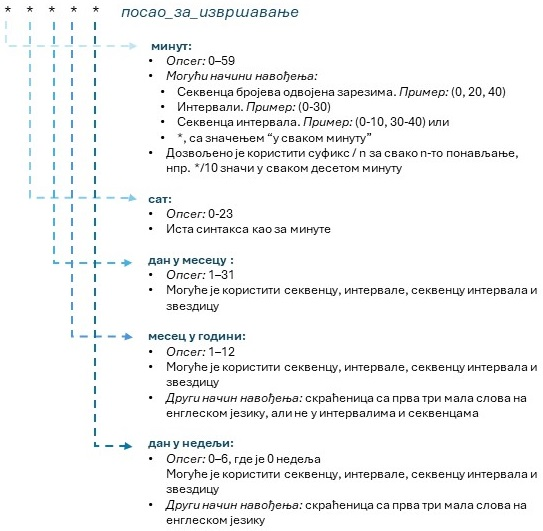
\includegraphics[scale=0.9]{assets/pictures/crontab_syntax.jpg}
  \caption{Синтакса конфигурационе датотеке \texttt{crontab}}
  \label{pic:crontab_syntax}
\end{figure}

На пример, следећи унос ће покренути скрипту \texttt{/home/user/script.sh} сваког дана у 2:30 ујутру:

\lstset{
  language=Python,
  basicstyle=\ttfamily,
  keywordstyle=\color{blue},
  frame=single
}
\begin{lstlisting}
    30 2 * * * /home/user/script.sh
\end{lstlisting}

\vspace{0.7cm}

У \textit{Django} апликацијама, планирање периодичних задатака може бити корисно за различите сврхе, као што су ажурирање база података, слање извештаја, чишћење привремених фајлова и друге периодичне активности. Један од популарних начина за управљање \textit{Cron} задацима у \textit{Django}-у је коришћење библиотеке \textit{django-crontab} \cite{django_crontab} која у позадини користи системски процес \textit{Cron}. \textit{Cron} задаци се додају у \texttt{settings.py} модул у оквиру \texttt{CRONJOBS} променљиве:

\lstset{
  language=Python,
  basicstyle=\ttfamily,
  keywordstyle=\color{blue},
  showstringspaces=false
}
\begin{lstlisting}
   CRONJOBS = [
       ('0 0 * * *', 'scheduled_job'),
       ('0 4 * * *', 'django.core.management.call_command',
       ['django_menagement_command']),
   ]
\end{lstlisting}

\noindentгде је \texttt{scheduled\_job} функција дефинисана у пројекту, a \texttt{dјango\_menagement\_command} уграђена \textit{Django menagement} команда (попут
\texttt{migrate}, \texttt{collectstatic}, ...) или прилагођена команда креирана од стране корисника.

Да би се дефинисани \textit{Cron} задаци извршавали, потребно их је додати са командом:

\lstset{
  language=Python,
  basicstyle=\ttfamily,
  keywordstyle=\color{blue}
}
\begin{lstlisting}
    python manage.py crontab add
\end{lstlisting}

Додате задатке је могуће уклонити наредном командом:

\lstset{
  language=Python,
  basicstyle=\ttfamily,
  keywordstyle=\color{blue}
}
\begin{lstlisting}
    python manage.py crontab remove
\end{lstlisting}

У апликацији \textit{Train Wiser} се користе два \textit{Cron} посла, један који на сваких сат времена уписује претходне активности корисника у базу и други за додавање детаља о новим активностима корисника.

\subsubsection{Мрежне куке}

\textit{Мрежне куке (енг. webhooks)} пружају начин за аутоматизацију комуникације између различитих сервиса путем \textit{HTTP} захтева. Када се одређени догађај деси у изворном систему, \textit{HTTP} захтев ће се аутоматски послати одредишном систему, најчешће садржећи корисне податке о догађају које одредишни систем захтева. Периодично слање захтева изворном систему ради провере да ли постоје нови или ажурирани догађаји (енг. \textit{pooling}) може бити неефикасно и оптеретити изворни систем. Коришћењем мрежних кука апликација ће добити информације о догађајима у реалном времену и искључиво онда када се догађаји десе. На тај начин се омогућава уштеда ресурса и ефикасна комуникација. 

Мрежне куке се јако често користе на \textit{SaaS (енг. software as a service)} платформама, будући да оне на основу активности које се дешавају подржавају креирање различитих типова догађаја. Да би апликација могла да добија \textit{HTTP} захтеве мрежних кука, потребно је да се региструје за догађаје за које их изворна платформа нуди, као и да обезбеди веб адресу на коју ће се захтеви слати \cite{webhooks_hookdeck, strava_webhooks}.

\paragraph{Коришћење мрежних кука у апликацији \textit{Train Wiser}} Апликација \textit{Strava} подржава мрежне куке за одређене промене у личним подацима и активностима корисника, и охрабрује све \textit{API} апликације да их користе. 

Када се догађај за који је мрежна кука везана догоди, \textit{POST} захтев се шаље на веб адресу дефинисану од стране апликације. Очекивано је да апликација узврати одговор са статусом 200 у оквиру 2 секунде. Уколико се то не деси, \textit{POST} захтев се понавља још максимално два пута, стога се саветује да се добијене информације обрађују асинхроно уколико је за обраду потебно више времена.

Да би се апликација регистровала за мрежне куке апликације \textit{Strava}, потребно је да се креира \textit{POST} захтев ка адреси
\url{https://www.strava.com/api/v3/push_subscriptions}. Очекивано је да захтев садржи параметре у \textit{URL} формату који укључују клијетски идентификатор и клијентски тајни кључ апликације, тј. податке за аутентификацију апликације за приступ \textit{Strava} ресурсима, поменуте у потпоглављу \ref{subsec:authorization_and_authentication}, затим, веб адресу повратног позива дефинисану од стране апликације на којој ће се захтеви слати \textit{(URL callback)} и јединствени токен дефинисан од стране власника апликације (\texttt{hub.verify\_token}) који ће апликација \textit{Strava} узвратити слањем верификационог \textit{GET} захтева ка \texttt{callback} адреси апликације. Верификациони \textit{GET} захтев поред токена садржи и два поља чије вредности су ниске карактера, \texttt{hub.mode} који је увек фиксне вредности \texttt{''subscribe''}, и \texttt{hub.challenge}, чија је вредност насумична ниска коју апликација узвраћа као одговор апликацији \textit{Strava}. Након слања одговора, апликација ће на рути са које је захтев за регистрацију послат добити \texttt{subscription\_id} који ће служити за проверу валидности приликом слања догађаја мрежних кука чиме се затвара процес регистрације \cite{strava_webhooks}.

Регистрација за мрежне куке апликације \textit{Strava} у апликацији \textit{Train Wiser} се покреће једнократно када апликација добије \textit{POST} захтев ка рути \\ \texttt{webhook\_subscription}. Као што је наведено у потпоглављу \ref{django:url_routing}, функције за обраду \textit{HTTP} захтева који се упућују ка одређеној рути се наводе у фајлу \texttt{urls.py}. У случају \texttt{webhook\_subscription} руте, одговарајућа функција је \texttt{webhook\_subscription} дефинисана у \texttt{views.py}. Ова функција ће проверити методу \textit{HTTP} захтева, и у случају \textit{POST} методе, послати \textit{POST} захтев ка адреси \url{https://www.strava.com/api/v3/push_subscriptions} са горенаведеним неопходним параметрима.

Функција \texttt{webhook\_callback} је задужена за обраду захтева са \texttt{callback} адресе. Према наведеном објашњењу, на ову адресу се шаљу верификациони \textit{GET} захтев за регистрацију апликације и догађаји мрежних кука у виду \textit{POST} захтева. У случају \textit{GET} захтева, функција ће проверити да ли су прослеђени параметри \texttt{hub.mode} и \texttt{hub.challenge}, као и да ли је верификациони токен једнак токену који је апликација проследила. Функција ће у одговору апликацији \textit{Strava} проследити параметар \texttt{hub.challenge} чиме успешно затвара процес верификације. Комплетирање процеса регистрације, након што \textit{Strava} пошаље параметар \texttt{subscription\_id} на руту \texttt{webhook\_subscription} ће одрадити функција \texttt{webhook\_subscription} чувањем идентификатора регистрације у табели \texttt{StravaSettings} у бази података. Осигуравање да се регистрација не ради више од једанпут се ради провером вредности овог параметра у табели на почетку позива функције. Регистрација ће се радити једино у случају да параметар већ није уписан, тј. уколико је вредност у табели једнака \texttt{NULL}.

Од догађаја за које се мрежне куке нуде од стране апликације \textit{Strava}, за формирање скупа података са активностима вежбача за апликацију \textit{Train Wiser} је релевантно креирање нових активности. 

Догађаји мрежних кука се обрађују на \texttt{callback} адреси за коју је задужена фјункција \texttt{webhook\_callback}. Након што корисник постави нову активност и апликација \textit{Train Wiser} добије \textit{POST} захтев, ова функција ће проверити \texttt{subscription\_id}, и у случају једнакости са вредношћу из \texttt{StravaSettings} табеле, уписати идентификаторе активности и вежбача чија активност је детектована у табелу за чување активности, \texttt{StravaActivity}. Дохватање детаљних информација о активности се ради коришћењем \textit{Django Cron} посла који ће на сваких сат времена у тридесетом минуту проверити да ли у бази постоје активности које нису попуњене, тј. садрже само идентификатор активности и страни кључ ка табели \texttt{StravaAthlete}. 


\subsection{Формирање скупа података са резултатима трка}
\label{subsec:scrapy_desc}

Скуп података са резултатима трка је формиран на основу резултата тркача доступних на сајтовима \href{https://www.runtrace.net}{\textit{runtrace.net}}, \href{https://www.trka.rs}{\textit{trka.rs}} и \href{https://www.bgdmarathon.org}{\textit{bgdmarathon.org}} за које је добијена потврда да се јавно доступни подаци могу користити у истраживачке сврхе. Подаци са ових сајтова су обрађени техником \textit{екстракције података (енг. scraping)}.

Преузимање података од стране програма на било који други начин осим директном комуникацијом програма са \textit{API}-ем странице представља технику екстракције података. Коришћење екстракције података уместо \textit{API}-ја се саветује када % тодо: види да ли да остављаш апи
\textit{API} није доступан или онда када јесте доступан, али формат података који пружа није одговарајући или постоји ограничење у обиму и учесталости захтева који се могу послати. Екстрактори веб података су ефикасан алат за прикупљање и обраду великих количина података са различитих веб страница \cite{web_scraping_with_python}.

Екстракција података са веб страница у апликацији \textit{Train Wiser} је одрађена коришћењем оквира \textit{Scrapy}. \textit{Scrapy} је оквир отвореног кода програмског језика \textit{Python} за обилазак и екстракцију структуираних података са \textit{HTML/XML} страница. Често се користи за анализу и процесирање података, надгледање активности, аутоматизацију тестирања и историјско архивирање. Главна одлика овог алата је да захтеве распоређује и процесира асинхроно што му омогућава веома брзо претраживање страница у односу на секвенциони приступ будући да се више захтева може процесирати у исто време уз постојање толеранције грешака. 

Oвај оквир пружа једноставан \textit{API} са доста могућности који је лако прилагодљив потребама програмера. Екстракција података се ради коришћењем проширених \textit{CSS} селектора и \textit{XPath} израза, док су \textit{JSON}, \textit{CSV} и \textit{XML} формат на располагању на излазу \cite{scrapy_doc}.


За потребе \textit{Train Wiser} апликације, екстрактовани подаци су експортовани у \textit{JSON} формат. На основу излазних фајлова екстрактора, оформњен је јединстевен \textit{JSON} фајл који садржи речник чији су кључеви имена тркача, а вредности речници чији кључеви представљају могуће дистанце трка (5, 7, 7.7, 10, 21 и 42 километара) и вредности листа са информацијама о резултатима тог учестника на свим тркама са одговарајућом километражом. Број укупно сакупљених података са сајтова приказан је у табели \ref{tbl:rezultati_trka}, док је укупан број тркача који имају информацију о учешћу на барем једној трци одржаној у Републици Србији 44077. 


\begin{table}[H]
\centering
\begin{tabular}{| >{\centering\arraybackslash} m{0.35\linewidth} | >{\centering\arraybackslash} m{0.35\linewidth} | >{\centering\arraybackslash} m{0.3\linewidth} |}
\hline
\textbf{Сајт} & \textbf{Укупан број резултата релевантних трка}  \\
\hline
\textit{runtrace.net} \rule{0pt}{1em} & 20908 \\
\hline
\textit{trka.rs} \rule{0pt}{1em} & 42833 \\
\hline
\textit{bgdmarathon.org} \rule{0pt}{1em} & 49742 \\
\hline
\end{tabular}
\caption{Број података са сајтова за резултате трка}
\label{tbl:rezultati_trka}
\end{table}



\section{Архитектура апликације}


Серверска страна апликације је подељена у више модуларних компоненти (\textit{Django} апликација) задужених за обраду унутрашње логике. У наредном тексту је објашњен начин рада и имплементације серверске апликације кроз компоненте које садржи.

\subsection{Компонтента за рад са корисничким налозима}\label{chapter:server-impl-registration-and-login-component}

За рад са корисничким налозима је задужена имплементирана компонента \texttt{users}. За креирање модела корисника одабрана је класа \texttt{AbstractUser} из библиотеке \texttt{django.contrib.auth.models} која служи као основа за креирање корисничког модела. У апликацији \textit{Train Wiser} је направљен модел \texttt{CustomUser} надоградњом овог модела додавањем страног кључа ка табели \texttt{StravaAthlete} и додатним ограничењима за атрибуте модела.

Коришћењем библиотеке \textit{Django OAuth Toolkit} \cite{django_oauth_toolkit} која обезбеђује све \textit{крајње тачке (енг. endpoints)}, податке и логику потребне за додавање \textit{OAuth2} функционалности \textit{Django} пројектима се омогућава пријављивање са клијентске стране на серверску преко протокола \textit{OAuth2}. Коришћен је тип одобрења (енг. \textit{grant type}) \textit{password} уз који клијентска апликација на основу корисничког имена и његове лозинке добија приступни токен који може користити у другим захтевима ка серверској апликацији намењеним за тог корисника. Поред приступног токена, апликација добија токен за обнову и време трајања приступног токена. Тип одобрења са разменом лозинке је погодан за коришћење само када су клијентска и серверска страна у истом власништву, док се за приступ апликацијама треће стране саветује коришћење поузданијих типова одобрења.

Библиотека \textit{Django OAuth Toolkit} има уграђене крајње тачке за пријављивање и одјављивање корисника, док је за регистрацију корисника потребно направити нову крајњу тачку апликације. \textit{API} који компонента \texttt{users} пружа, поред регистровања корисника, омогућава једноставно добијање информација о ауторизованом кориснику, мењање параметара корисничког профила и брисање корисничког налога коришћењем класе \texttt{generics.RetrieveUpdateDestroyAPIView} оквира \textit{Django REST Framework}.


\subsection{Компонтента за руковање захтевима ка апликацији \textit{Strava}}

Компонента \texttt{strava\_gateway} садржи имплементацију за три модела, \\ \texttt{StravaAthlete}, \texttt{StravaActivity} и \texttt{StravaSettings}. Модел \texttt{StravaAthlete} садржи идентификатор корисника на апликацији \textit{Strava} и податке за приступ овој апликацији које чине приступни токен, токен за обнову и време истека приступног токена. Додатно, у овом моделу се чувају подаци о границама за сваку зону срчаног пулса корисника који се добијају засебним \textit{GET} захтевом и поље \texttt{backfill\_progress} за чување информације докле се стигло са допремањем претходних активности корисника у базу након ауторизације са апликацијом \textit{Strava}. Ово поље је иницијално постављено на 0, а претходне активности корисника ће се допремати преко \textit{Cron} задатка све док вредност овог поља не постане \texttt{NULL} након што су све активности сачуване у бази. Ако се у току једне итерације позивања \textit{Cron} задатка не допреме све активности, \texttt{backfill\_progress} се поставља на вредност датума почетка последње допремњене активности како би \textit{Cron} задатак знао одакле да настави при следећем позиву.

Модел \texttt{StravaActivity} садржи све информације о активностима које су иницијално доступне за активности на \textit{Strava API}-ју и додатна поља попут просечне зоне срчаног пулса, поље за чување информације да ли је активност трка и заокружену вредност дистанце трке. Поље за просечну зону срчаног пулса у току активности се израчунава на основу граница зона срчаног пулса из модела \texttt{StravaAthlete} и вредности просечног срчаног пулса у току активности. Ово поље је додато како би се лакше разликовао тип тренинга и јер се границе зона разликују од особе до особе, те је и приликом увида у туђе активности јасније колико је активност захтевна. Табела \texttt{StravaActivity} садржи страни кључ ка табели \texttt{StravaAthlete} који је повезан преко поља за индентификацију корисника.

Модел \texttt{StravaSettings} има два поља, \texttt{setting\_key} и \texttt{setting\_value}. У овој табели се чува \texttt{subscription\_id} потребан за мрежне куке апликације \textit{Strava}, а табела се може допунити другим подешавањима по потреби.

Ова компонента не пружа \textit{API} за директан рад са клијентском апликацијом већ обезбеђује доступност прилагођених података са апликације \textit{Strava} другим компонентама и функције за обраду захтева ка овој апликацији које смо описали у потпоглављима \ref{subsec:authorization_and_authentication} и \ref{subsec:activities_dataset}. Такође, у оквиру ове компоненте је направљена \textit{Django} команда за експортовање свих активности корисника у \textit{CSV} фајл што омогућава њихову прилагоднију употребу за различите анализе и развој нових функционалности. Команда се позива са:

\lstset{
  language=Python,
  basicstyle=\ttfamily,
  keywordstyle=\color{blue},
  frame=single
}
\begin{lstlisting}
    python manage.py export_to_csv
\end{lstlisting}

\subsection{Компонтента за генерисање планова тренинга}

Компонента \texttt{trainings} пружа \textit{API} који на улазу прима дистанцу трке и жељени временски резултат корисника, а враћа до највише пет планова тренинга који одговарају тренинзима корисника апликације који су остварили најприближније резултате траженом. За дистанце дужине 5km, компонента враћа шестонедељне планове, за дистанце дужине 7km, 7.7km и 10km осмонедељне, 21km дванестонедељне и за 42km шеснаестонедељне. Планови тренинга се генеришу на основу табеле \texttt{StravaActivity} из базе података тако што се посматрају сви тркачки резултати на тркама жељене дистанце и узима се пет најприближнијих резултата циљаном. Затим се израчунава број дана трајања тренинг плана за тражену дистанцу и за корисника који је остварио тај резултат се узимају сви његови тренинзи у оквиру тог периода. 

Осим постигнутог резултата на трци, алгоритам враћа и процентуалну разлику у границама зона срчаног пулса корисника за кога се генерише план тренинга у односу на зоне корисника коме припадају тренинзи на основу којих се тренинг план предлаже. Ова разлика се доставља ако су оба корисника повезала апликацију \textit{Train Wiser} са апликацијом \textit{Strava} и имају доступну информацију о границама зона срчаног пулса.

\textit{API} компоненте као одговор враћа речник чији кључеви представљају резултат на трци уз опциону разлику у зонама срчаног пулса, а вредности тренинзи који су претходили резултату одређеног корисника апликације.


\subsection{Компонтента за статистичке извештаје о тренинзима}

Компонента \texttt{stats} пружа \textit{API} са извештајима о тренинзима за задати месец и годину корисника која се прослеђује у оквиру \textit{URL} путање. Ова компонента израчунава које недеље у години су покривене одабраним месецом и за њих даје информације о свим тренинзима које укључују тип тренинга, пређену дистанцу, трајање тренинга, просечну зону срчаног пулса и датум тренинга. Такође, за сваки тип тренинга се прави месечни извештај са укупним трајањем, укупном дистанцом и просечном зоном срчаног ритма свих тренинга тог типа у оквиру одабраних недеља.

Информације које компонента пружа се израчунавају и генеришу на основу података из табеле \texttt{StravaActivity}. Стога, да би клијентска апликација могла да користи \textit{API} ове компоненте за тренутног корисника, потребно је да је корисник аутентификован и да има налог на апликацији \textit{Strava} коју је повезао са апликацијом \textit{Train Wiser}. 

\subsection{Компонтента за предикцију резултата на наредној трци}

Предикција резултата на трци, за коју је задужена компонента \\
\texttt{results\_predictor}, је одрађена коришћењем алгоритма \textit{Експоненцијално пондерисана покретна средина (енг. Exponentially Weighted Moving Average, EMWA)} \cite{ewma} који се користи за моделовање и опис временских серија. 

Основна идеја овог алгоритма је да се свака вредност у серији пондерише фактором који експоненцијално опада како се удаљава од тренутног временског тренутка. Формула на којој се \textit{EWMA} заснива је:
\[
\begin{aligned}
\text{EWMA}_t = \alpha \cdot x_t + (1 - \alpha) \cdot \text{EWMA}_{t-1}
\end{aligned}
\]

Потребно је да корисник обезбеди \textit{параметар изглађивања $\alpha$ (енг. smoothing factor)} који узима вредности између 0 и 1. 

\begin{itemize}
    \item Када је $ \alpha > 0.5 $ -- Алгоритам брже реагује на промене у подацима
    \item Када је $ \alpha < 0.5 $ -- Брзина опадања тежине старијих података је мања у односу на случај када је $\alpha$ већа од 0.5
\end{itemize}

Уколико развијемо рекурзивну \textit{EWMA} формулу,

\[
\begin{aligned}
\text{EWMA}_t &= \alpha \cdot x_t + (1 - \alpha) \cdot \text{EWMA}_{t-1} \\
              &= \alpha \cdot x_t + (1 - \alpha) \cdot \left[\alpha \cdot x_{t-1} + (1 - \alpha) \cdot \text{EWMA}_{t-2}\right] \\
              &= \alpha \cdot x_t + \alpha \cdot (1 - \alpha) \cdot x_{t-1} + (1 - \alpha)^2 \cdot \text{EWMA}_{t-2} \\
              &\vdots \\
              &= \alpha \cdot x_t + \alpha \cdot (1 - \alpha) \cdot x_{t-1} + \alpha \cdot (1 - \alpha)^2 \cdot x_{t-2} + \dots \\
              &\quad + \alpha \cdot (1 - \alpha)^k \cdot x_{t-k} + \dots
\end{aligned}
\]

\noindent можемо закључити да тежина за податак $x_{t-k}$ износи $\alpha \cdot (1 - \alpha)^k$, а како је $\alpha$ између 0 и 1, тежина постаје мања што је $k$ веће, тј. тежина података има мању вредност што су подаци старији.

За компоненту \texttt{results\_predictor} је одабрана имплементација овог алгоритма библиотеке \textit{Pandas} sa параметром $\alpha=0.9$. Компонента пружа \textit{API} који на основу имена тркача (које добија из модела \texttt{CustomUser} на основу приступног токена) и дистанце трке даје процену за резултат на наредној трци на основу историјских података о учешћу на тркама исте дистанце у Републици Србији чије преузимање смо описали у поглављу \ref{subsec:scrapy_desc}.


\section{Јавни интерфејс за програмирање апликација}

Спецификација јавног интерфејса за програмирање апликација који је имплементиран на серверској страни за приступ од стране клијентске апликације је дата у табели \ref{tbl:api}. За све захтеве из табеле почев од захтева за добијање података о кориснику је потребно проследити приступни токен корисника кроз заглавље захтева на следећи начин:

\lstset{
  language=Python,
  basicstyle=\ttfamily,
  keywordstyle=\color{blue},
  showstringspaces=false
}
\begin{lstlisting}
    "Authorization": "Bearer " + token
\end{lstlisting} 

\newpage

\begin{longtable}{| 
>{\centering\arraybackslash} m{0.11\linewidth} |
>{\centering\arraybackslash} m{0.315\linewidth} | 
>{\raggedright\arraybackslash} m{0.28\linewidth} 
|>{\raggedright\arraybackslash} m{0.28\linewidth}|}
\hline
\multicolumn{4}{| c |}{
	Регистрација новог корисника 
}\\*
\hline
\hline
\textbf{HTTP метода} & \textbf{Путања ресурса} & \textbf{Параметри тела захтева} & \textbf{Тело одговора} \\
\hline
POST & \texttt{api/users/register/} & 
$\cdot$ \textit{\texttt{username}}: \texttt{String}\newline
$\cdot$  \textit{\texttt{email}}: \texttt{String}\newline
$\cdot$ \textit{\texttt{first\_name}}: \texttt{String}\newline
$\cdot$ \textit{\texttt{last\_name}}: \texttt{String}\newline
$\cdot$ \textit{\texttt{password}}: \texttt{String}\newline
$\cdot$ \textit{\texttt{birth\_date}}: \texttt{String} 
& 
$\cdot$ \textit{\texttt{user\_id}}: \texttt{Integer} 
\\
\hline
\hline
\multicolumn{4}{| c |}{
    Пријављивање корисника
}\\*
\hline
\hline
\textbf{HTTP метода} & \textbf{Путања ресурса} & \textbf{Параметри тела захтева} & \textbf{Тело одговора} \\
\hline
POST & \texttt{o/token/} & 
$\cdot$ \textit{\texttt{username}}: \texttt{String}\newline
$\cdot$ \textit{\texttt{password}}: \texttt{String}\newline
$\cdot$ \textit{\texttt{client\_id}}: \texttt{String}\newline
$\cdot$ \textit{\texttt{client\_secret}}: \texttt{String}\newline
$\cdot$ \textit{\texttt{grant\_type}}: \texttt{String} & 
$\cdot$ \textit{\texttt{access\_token}}: \texttt{String}\newline
$\cdot$ \textit{\texttt{expires\_in}}: \texttt{long}\newline
$\cdot$ \textit{\texttt{token\_type}}: \texttt{String}\newline
$\cdot$ \textit{\texttt{scope}}: \texttt{String}\newline
$\cdot$ \textit{\texttt{refresh\_token}}: \texttt{String} \\
\hline
\hline

\multicolumn{4}{| c |}{
Одјављивање корисника
}\\*
\hline
\hline
\textbf{HTTP метода} & \textbf{Путања ресурса} & \textbf{Параметри тела захтева} & \textbf{Тело одговора} \\
\hline
POST & \texttt{o/revoke\_token/} & 
$\cdot$ \textit{\texttt{client\_id}}: \texttt{String}\newline
$\cdot$ \textit{\texttt{client\_secret}}: \texttt{String}\newline
$\cdot$ \textit{\texttt{token}}: \texttt{String} & \multicolumn{1}{c|}{/} \\
\hline
\hline

\multicolumn{4}{| c |}{
	Добијање података о кориснику
}\\*
\hline
\hline
\textbf{HTTP метода} & \textbf{Путања ресурса} & \textbf{Параметри захтева} & \textbf{Тело одговора} \\
\hline
GET & \texttt{api/users/me/} & \multicolumn{1}{c|}{/} & $\cdot$ \textit{\texttt{strava\_athlete\_id}}: \texttt{Integer}\newline
$\cdot$ \textit{\texttt{username}}: \texttt{String}\newline
$\cdot$ \textit{\texttt{email}}: \texttt{String}\newline
$\cdot$ \textit{\texttt{first\_name}}: \texttt{String}\newline
$\cdot$ \textit{\texttt{last\_name}}: \texttt{String}\newline
$\cdot$ \textit{\texttt{password}}: \texttt{String}\newline
$\cdot$ \textit{\texttt{birth\_date}}: \texttt{String} \\
\hline

\hline
\multicolumn{4}{| c |}{
Мењање корисничких података
}\\*
\hline
\hline
\textbf{HTTP метода} & \textbf{Путања ресурса} & \textbf{Параметри тела захтева} & \textbf{Тело одговора} \\
\hline
PATCH & \texttt{api/users/me/} & Мапа типа \texttt{Map<String, Object>} са пољима које је потребно поставити на нове вредности. Вредности кључева који се могу користити одговарају вредностима из наредне колоне. & 
$\cdot$ \textit{\texttt{strava\_athlete\_id}}: \texttt{Integer}\newline
$\cdot$ \textit{\texttt{username}}: \texttt{String}\newline
$\cdot$ \textit{\texttt{email}}: \texttt{String}\newline
$\cdot$ \textit{\texttt{first\_name}}: \texttt{String}\newline
$\cdot$ \textit{\texttt{last\_name}}: \texttt{String}\newline
$\cdot$ \textit{\texttt{password}}: \texttt{String}\newline
$\cdot$ \textit{\texttt{birth\_date}}: \texttt{String} \\
\hline
\hline

\multicolumn{4}{| c |}{
    Брисање корисничког налога
}\\*
\hline
\hline
\textbf{HTTP метода} & \textbf{Путања ресурса} & \textbf{Параметри захтева} & \textbf{Тело одговора} \\
\hline
DELETE & \texttt{api/users/me/} & \multicolumn{1}{c|}{/} & \multicolumn{1}{c|}{/} \\
\hline
\hline

\multicolumn{4}{| c |}{
    Предлагање планова тренинга за остваривање одређених резултата
}\\*
\hline
\hline
\textbf{HTTP метода} & \textbf{Путања ресурса} & \textbf{Параметри захтева} & \textbf{Тело одговора} \\
\hline
GET & \texttt{api/trainings/} & 
$\cdot$ \textit{\texttt{goal\_time}}: \texttt{int}\newline 
$\cdot$ \textit{\texttt{race\_distance}}: \texttt{float} & Мапа типа  \texttt{Map<String, 
List<List<List<
TrainingPlan>>>>} где је \texttt{TrainingPlan} речник са пољима следећих типова: \newline
$\cdot$ \textit{\texttt{activity\_type}}: \texttt{String}\newline
$\cdot$ \textit{\texttt{distance}}: \texttt{float}\newline
$\cdot$ \textit{\texttt{duration}}: \texttt{int}\newline
$\cdot$ \textit{\texttt{avg\_hr\_zone}}: \texttt{int} \\
\hline
\hline

\multicolumn{4}{| c |}{
    Предикција резултата на наредној трци
}\\*
\hline
\hline
\textbf{HTTP метода} & \textbf{Путања ресурса} & \textbf{Параметри захтева} & \textbf{Тело одговора} \\
\hline
GET & \texttt{api/result\_prediction/} & 
$\cdot$ \textit{\texttt{race\_distance}}: \texttt{Sting} & 
$\cdot$ \textit{\texttt{race\_result}}: \texttt{Sting} \\
\hline
\hline


\multicolumn{4}{| c |}{
    Месечна статистика тренинга
}\\*
\hline
\hline
\textbf{HTTP метода} & \multicolumn{2}{| c |}{\textbf{Путања ресурса}} & \textbf{Тело одговора} \\
\hline
GET & \multicolumn{2}{| c |}{\texttt{api/stats/<int:year>/<int:month>/}} & 
$\cdot$ \textit{\texttt{training\_weeks}}: \texttt{Map<String, WeekSummary\textsuperscript{*}>} \\
\hline


\caption{Јавни интерфејс за програмирање апликација} \label{tbl:api} 
\end{longtable} 


\noindent \textsuperscript{*}Опис за \texttt{WeekSummary}:

\lstset{
  language=Java,
  basicstyle=\ttfamily,
  keywordstyle=\color{blue},
  showstringspaces=false
}
\begin{lstlisting}
    WeekSummary =  {
        "activities": List<Activity>,
        "summary": Map<String, ActivitySummary>
    };
    
    Activity = {
        "activity_type": String,
        "distance": float,
        "duration": int,
        "avg_hr_zone": int,
        "start_date": String
    };
    
    ActivitySummary = {
        "total_duration": int,
        "total_distance": float,
        "avg_hr_zone": int
    };
\end{lstlisting}

\chapter{Клијентска страна апликације \textit{Train Wiser}}\label{chapter:impl-client-app}

Функционалности имплементиране на серверској страни, клијентска апликација чини погодним за коришћење од стране корисника кроз графички кориснички интерфејс. У овом поглављу ћемо се детаљније упознати са њеном архитектуром, радним током и представити случајеве употребе.


\section{Aрхитектура апликације}

За израду клијентске стране апликације, коришћен је програмски језик \textit{Java} уз развојни оквир \textit{Android}. Апликација садржи \textit{Android} активности и њихове распореде за сваки екран који се приказује кориснику, класе за комуникацију са \textit{API}-јем и класе за додатне функционалности.

Комуникација са серверском апликацијом је остварена коришћењем библиотеке \textit{Retrofit}. \textit{Retrofit} \cite{retrofit} је библиотека за типизоване \textit{HTTP} клијенте у \textit{Android} и \textit{Java} апликацијама, коју је развила компанија \textit{Square}. Омогућава лако и ефикасно обављање \textit{REST API} позива, претварајући \textit{HTTP API} у \textit{Java} интерфејс са прецизно дефинисаним типовима података. 

Као што је наведено у потпоглављу \ref{chapter:server-impl-registration-and-login-component}, клијентска апликација на основу прослеђеног корисничког имена и лозинке корисника, добија приступни токен, токен за обнову и време истицања приступног токена за тог корисника. Да би корисник остао пријављен на апликацији и након што изађе из ње, потребно је сачувати ове податке и онда када апликација није активна. За ово је одабран \textit{SharedPreferences API} \cite{shared_preference} који је погодан за чување једноставних података. Подаци се складиште у паровима кључ-вредност и чувају у \textit{XML} датотеци у меморији за податке апликације на уређају корисника, а \textit{SharedPreferences API} обезбеђује методе за читање и упис сачуваних података.

Како би подаци о кориснику били доступни у свим тренуцима рада апликације, направљена је \texttt{Singleton} класа \texttt{ProfileSingleton} за чување параметара корисничког профила који се допремају преко \textit{API}-ја. Приликом покретања апликације, атрибути ове класе се постављају учитавањем најновијег стања са серверске апликације, а освежавају и постављају на иницијалну празну вредност у другим фазама рада апликације описаним у наредном потпоглављу.


\section{Радни ток апликације}

Ток рада апликације креће од иницијалне \textit{Android} активности која проверава да ли је корисник већ пријављен и, уколико није, преусмерава га на екран за пријављивање на апликацију. На овом екрану се налазе поља за унос података за аутентификацију и опција за преусмерење на екран за регистрацију уколико корисник нема креиран налог. Изглед активности за пријављивање корисника је приказан на слици \ref{pic:user_log_in}.
Активност за регистрацију садржи уносе за корисничко име, лозинку, потврду лозинке, \textit{e-mail} адресу и датум рођења, приказана је слици \ref{pic:user_sign_up}.


\begin{figure}[h]
  \centering
  \begin{minipage}{0.45\textwidth}
    \centering
    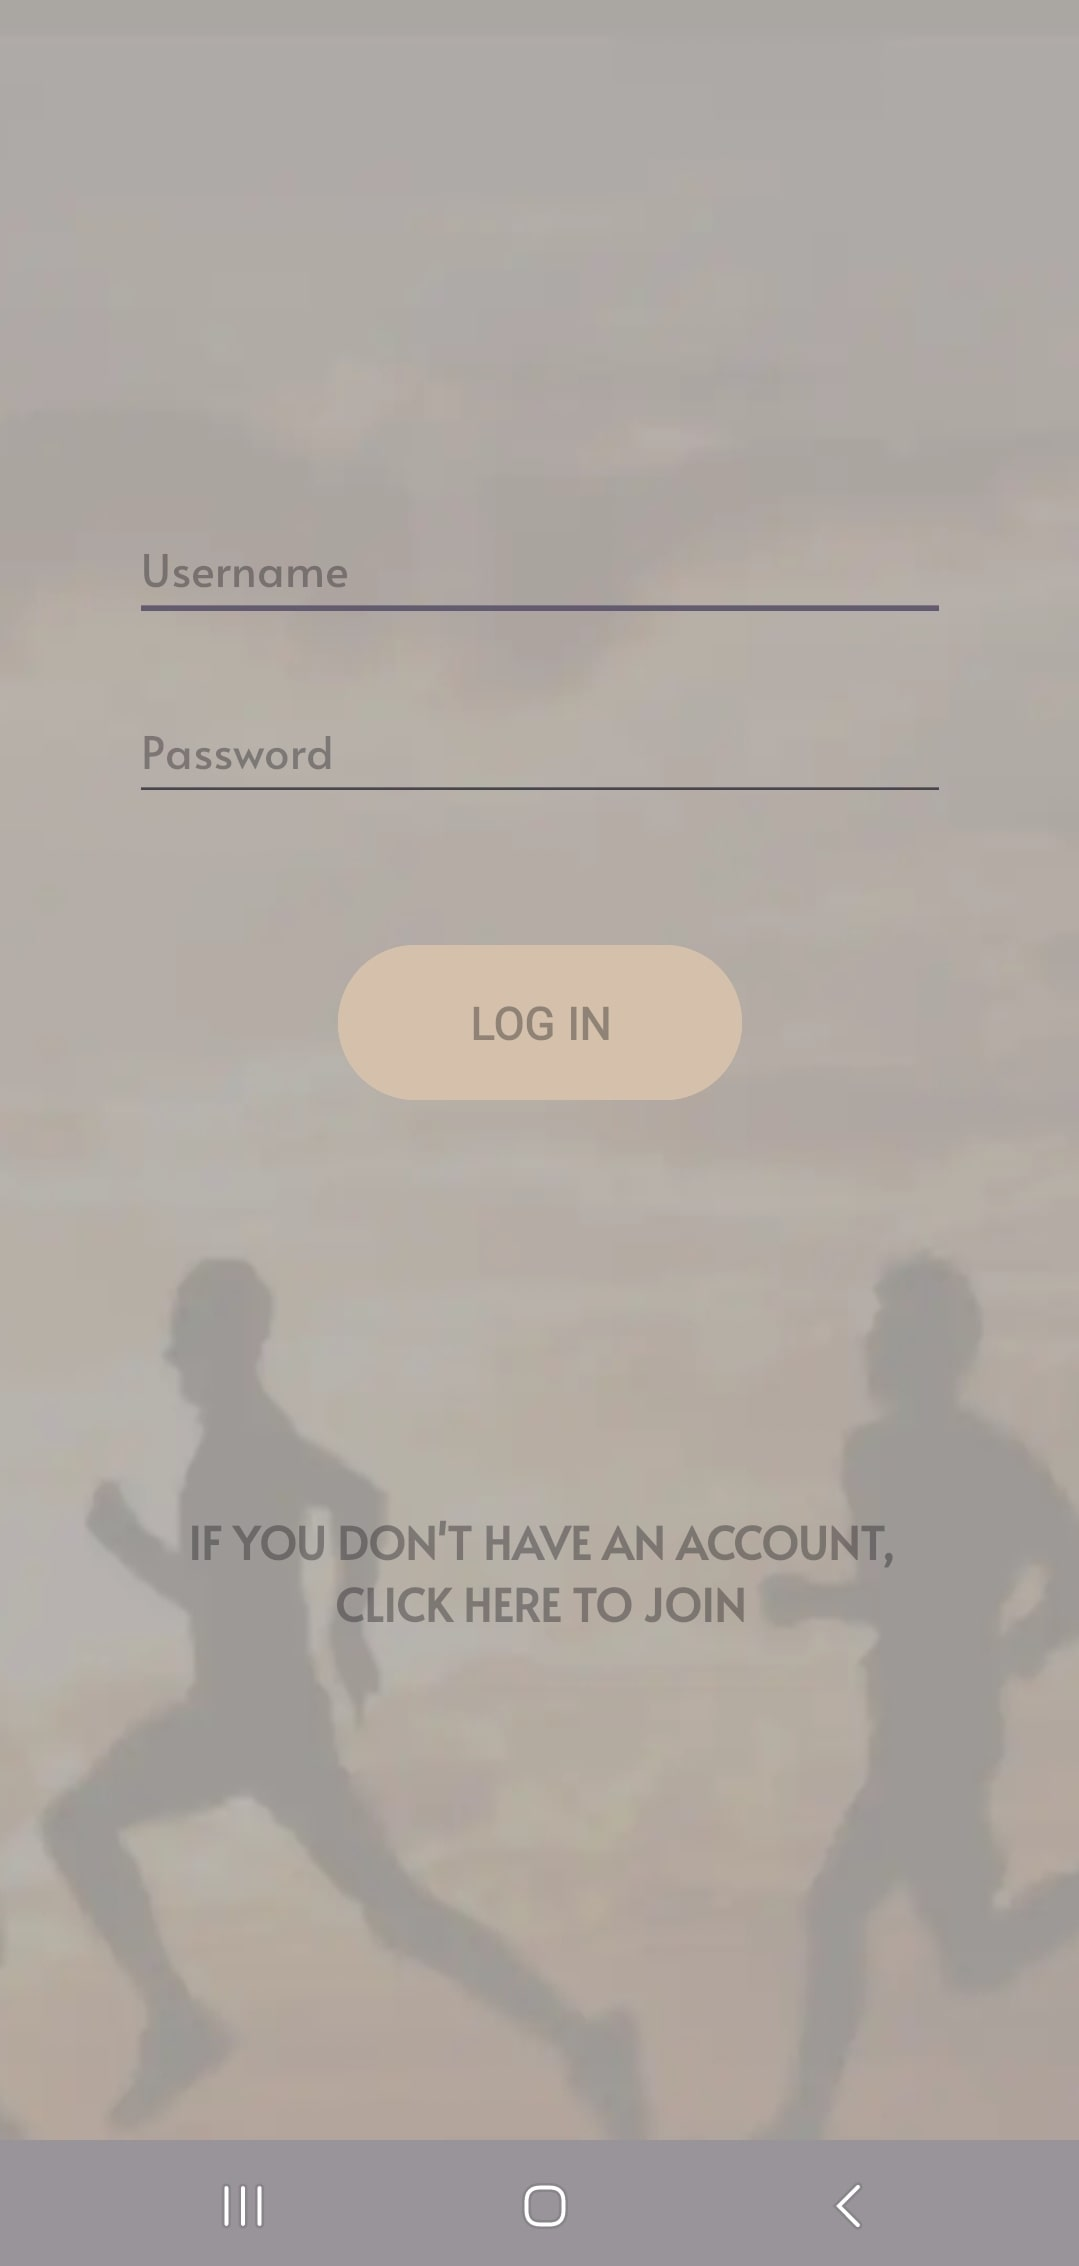
\includegraphics[scale=0.12]{assets/pictures/app_screenshots/login.jpg}
    \caption{Пријављивање корисника на апликацију \textit{Train Wiser}}
    \label{pic:user_log_in}
  \end{minipage}
  \hspace{0.05\textwidth} 
  \begin{minipage}{0.45\textwidth}
    \centering
    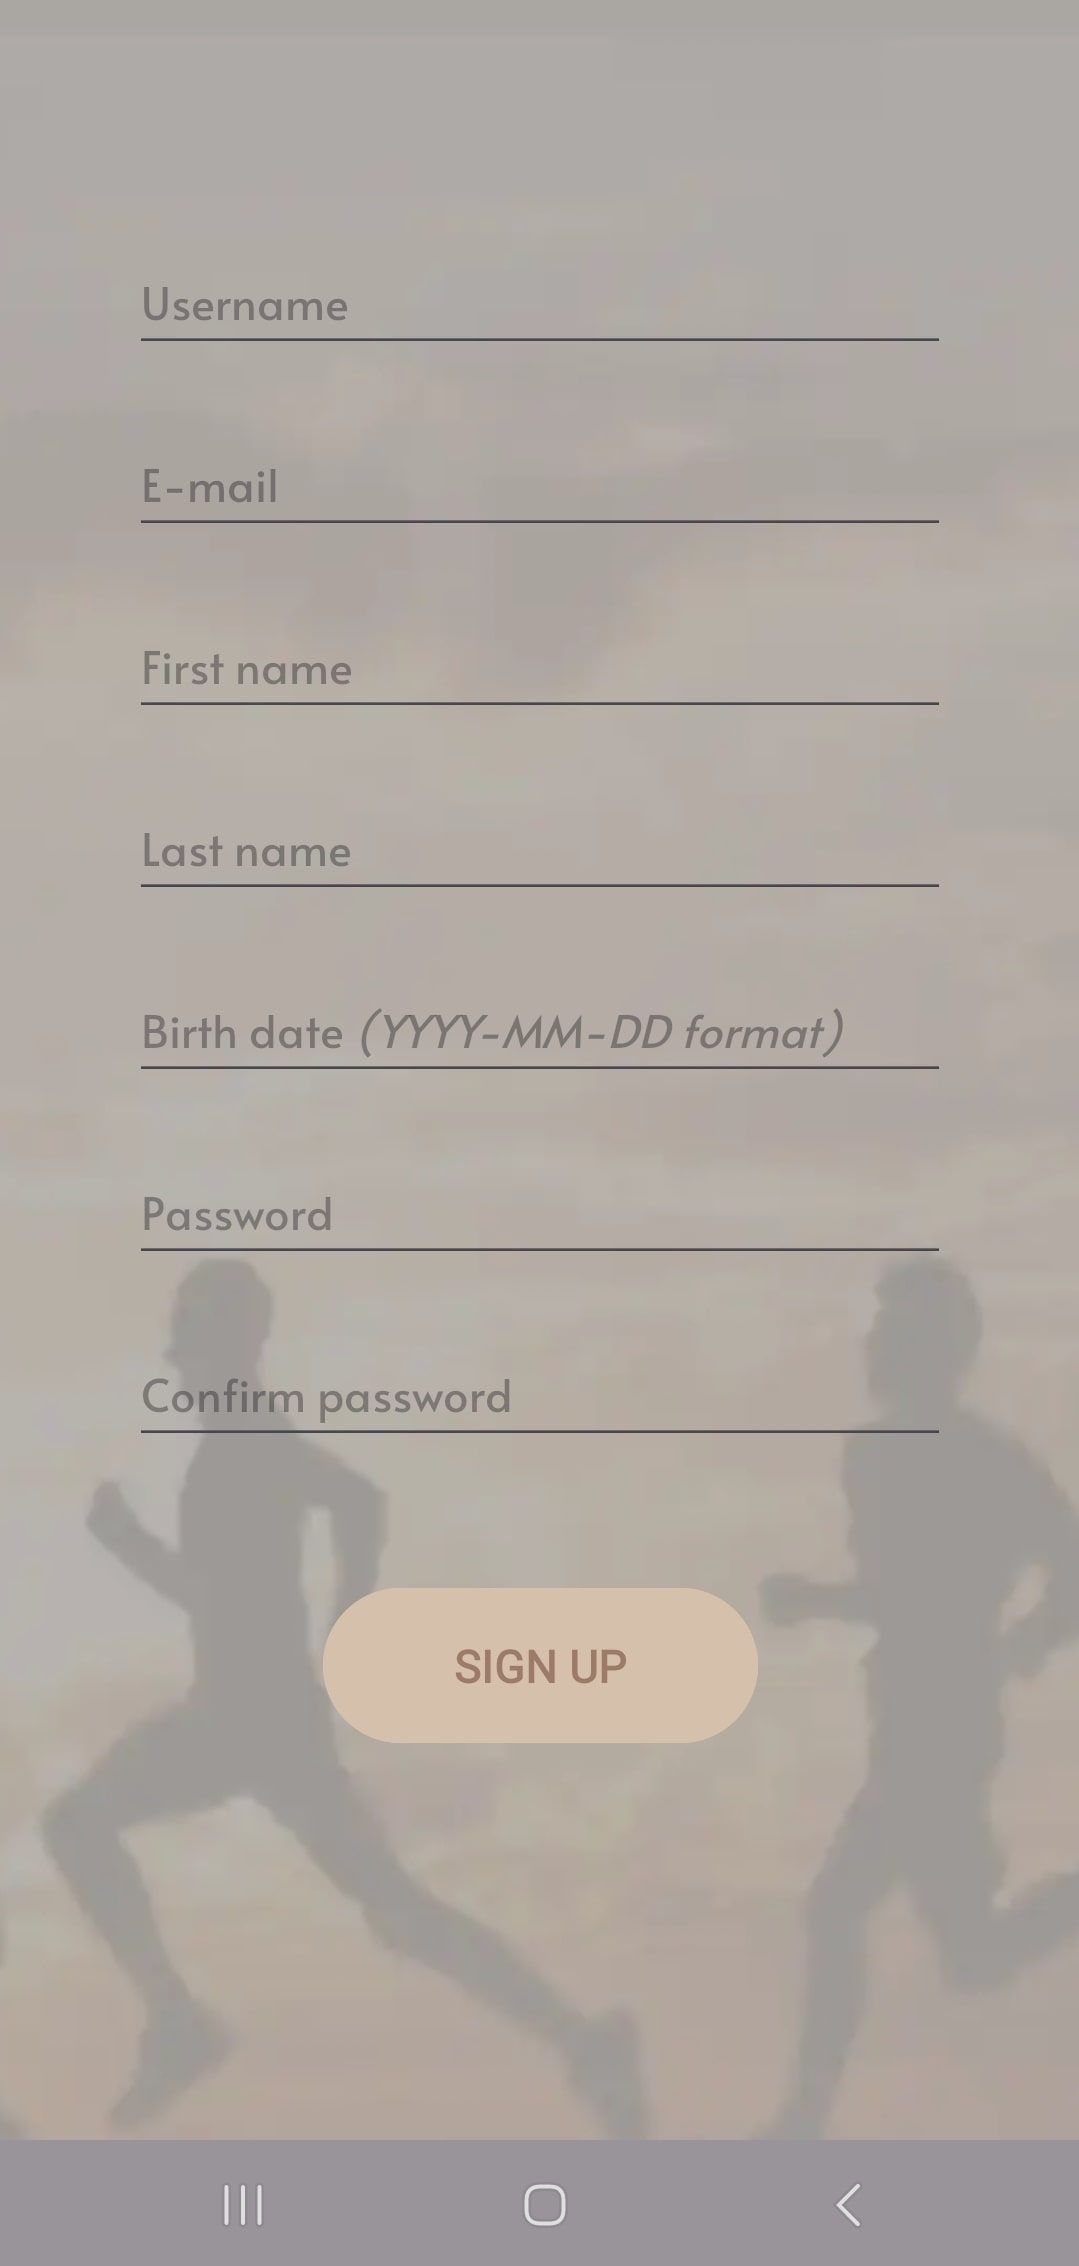
\includegraphics[scale=0.12]{assets/pictures/app_screenshots/signup.jpg}
    \caption{Регистрација корисника на апликацију \textit{Train Wiser}}
    \label{pic:user_sign_up}
  \end{minipage}
\end{figure}

Уколико је корисник већ пријављен, као и након пријављивања, биће преусмерен на екран са главним менијем за избор услуга. Главни мени је приказан на слици \ref{pic:app_main_menu} и садржи групу примарних опција за генерисање плана тренинга, предикцију резултата на наредној трци и приказивање месечне статистке тренинга. Дугме за генерисање плана тренинга отвара нови екран који за одређену дистанцу и резултат, посредством \textit{API} позива ка серверској страни, враћа избор за до највише пет типова вишенедељних планова тренинга које корисник може прегледати кликом на дугме које одговара плану тренинга са резултатом за који је заинтересован (слике \ref{pic:training_plan}). Снимци екрана за предикцију резултата у случају различитих одговора од стране сервера су приказани на слици \ref{pic:race_prediction}. У оквиру ове \textit{Android} активности, апликација ће кориснику пружити предикцију његовог резултата на одабраној дистанци или информацију да његови резултати, односно резултати за ту дистанцу, нису пронађени међу доступним резултатима у оквиру апликације. Изглед екрана за месечну статистику тренинга је приказан на сликама \ref{pic:training_stats}.

\begin{figure}[h]
  \centering
  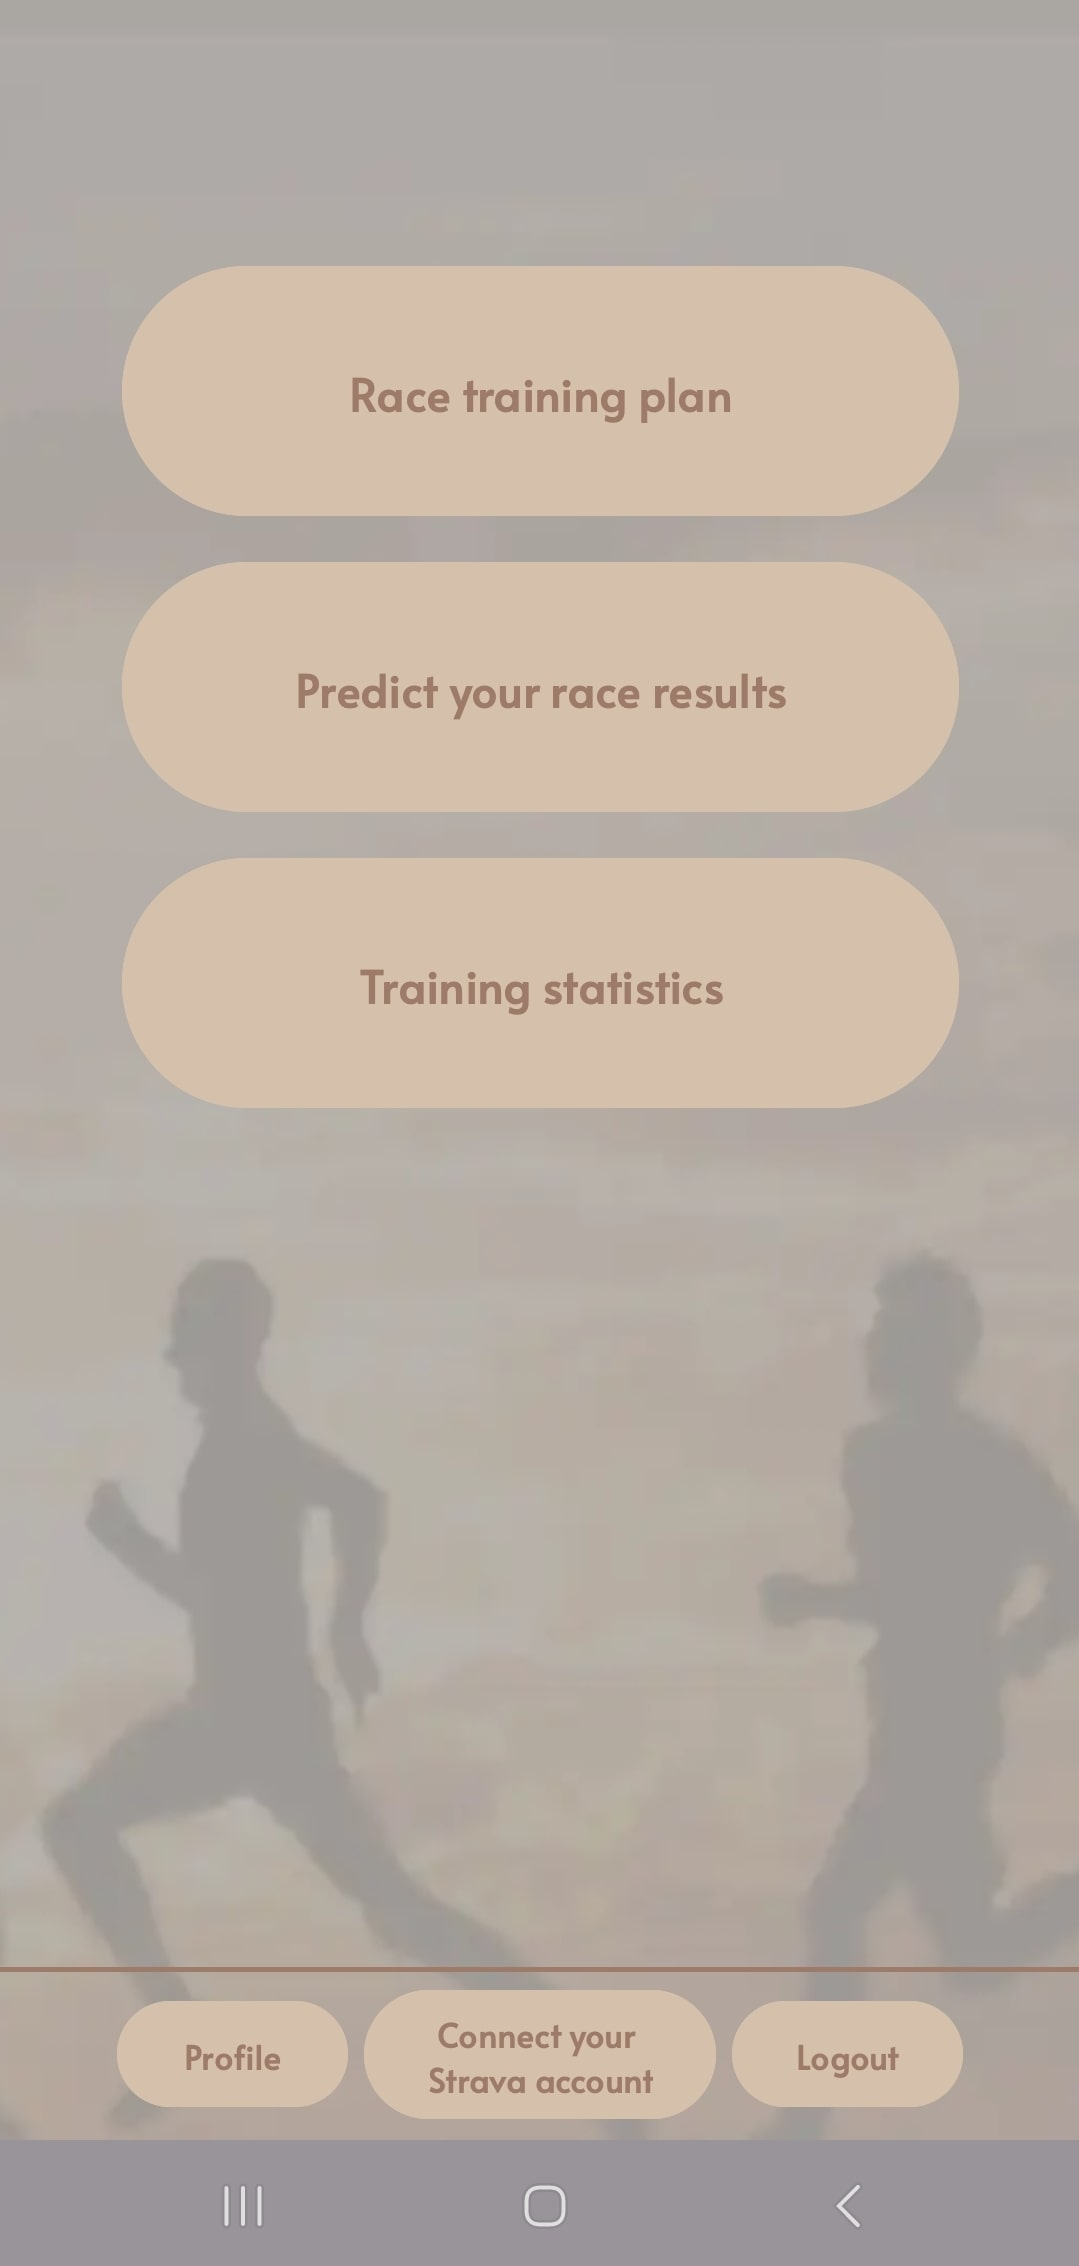
\includegraphics[scale=0.1]{assets/pictures/app_screenshots/main_menu.jpg}
  \caption{Изглед главног менија апликације \textit{Train Wiser}}
  \label{pic:app_main_menu}
\end{figure}

\begin{figure}[h]
  \centering
  \begin{minipage}{0.23\textwidth}
    \centering
    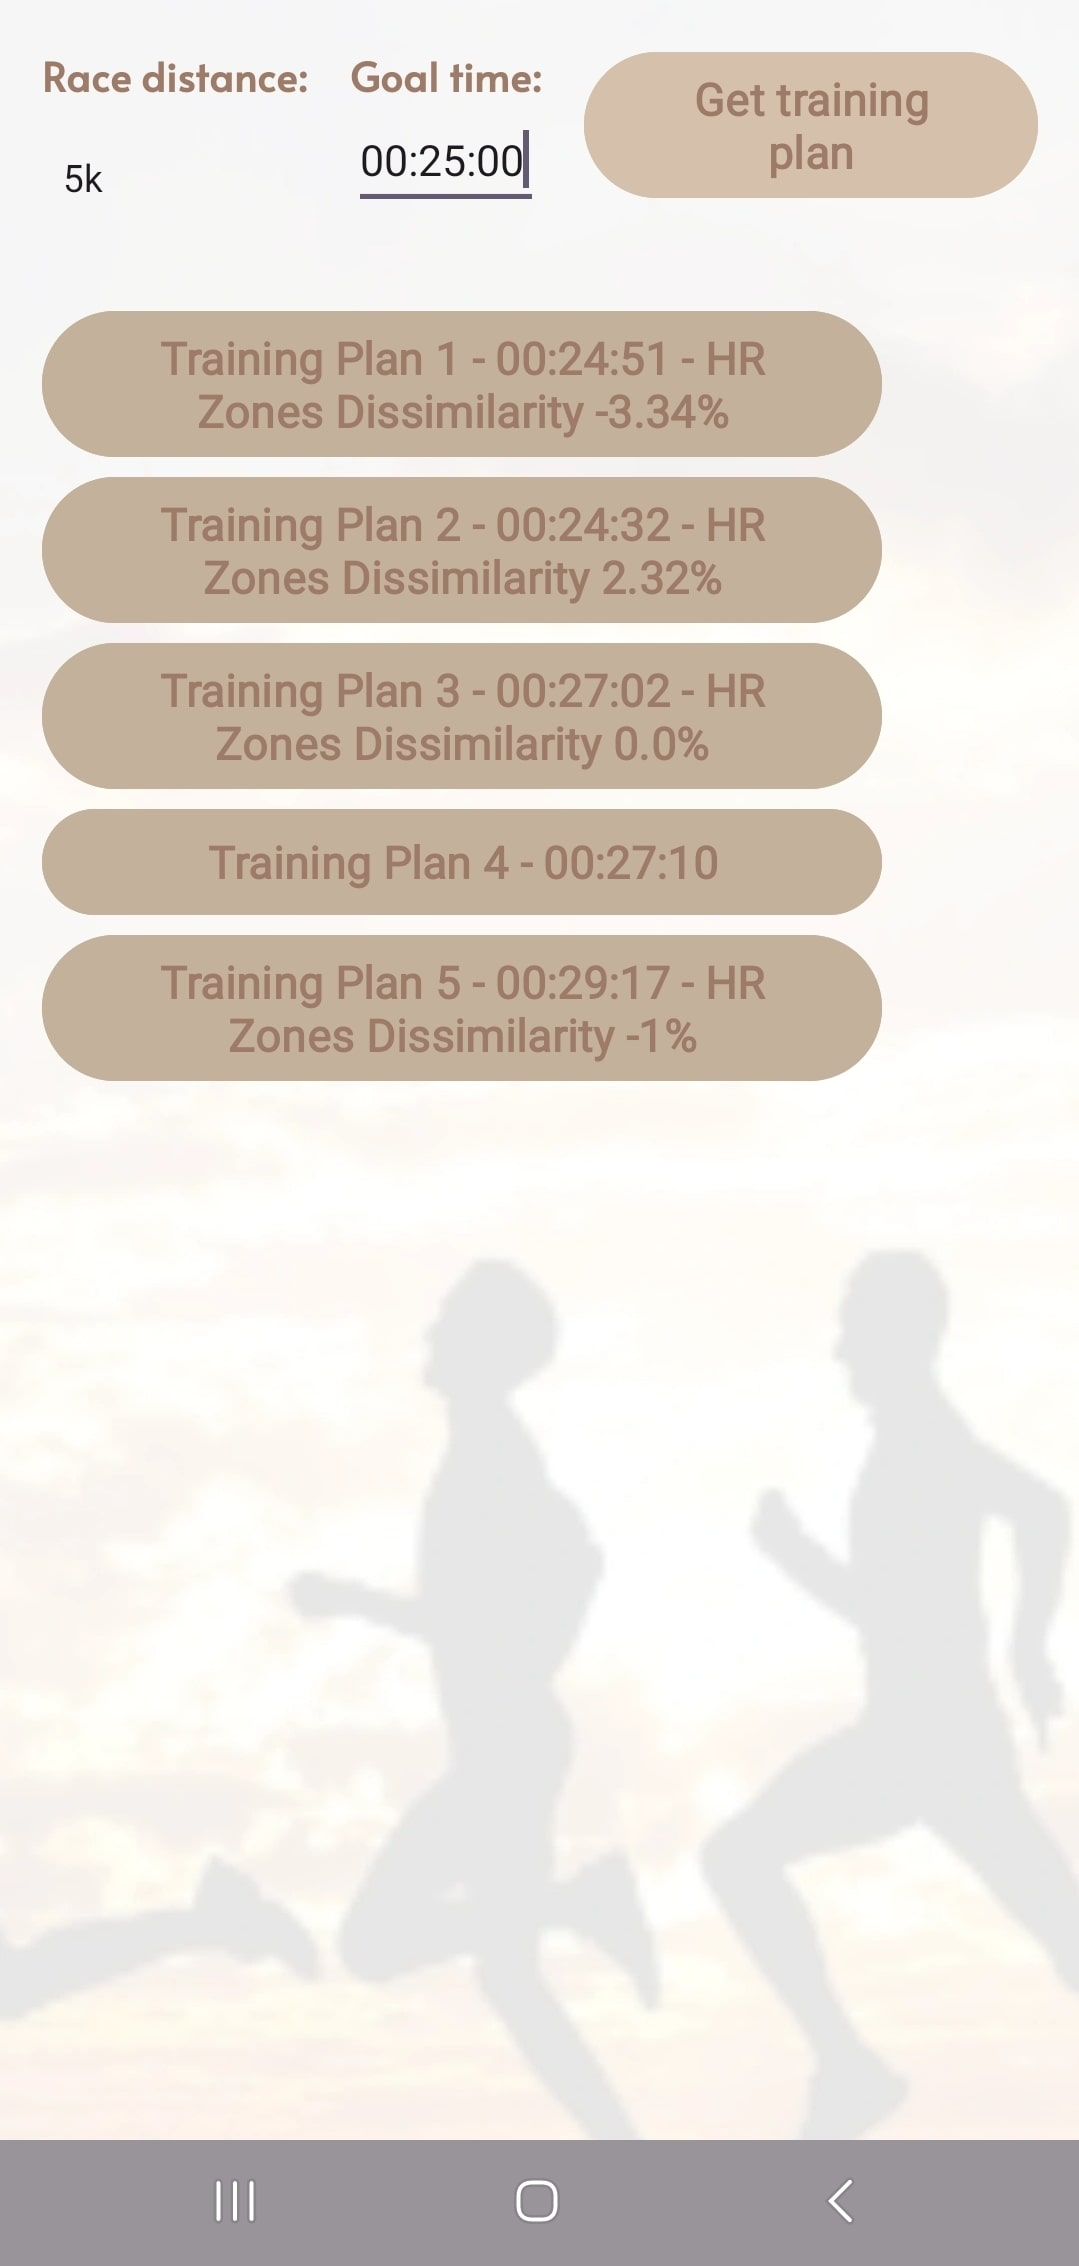
\includegraphics[width=\textwidth]{assets/pictures/app_screenshots/training_plan_0.jpg}
  \end{minipage}
  \hfill
  \begin{minipage}{0.23\textwidth}
    \centering
    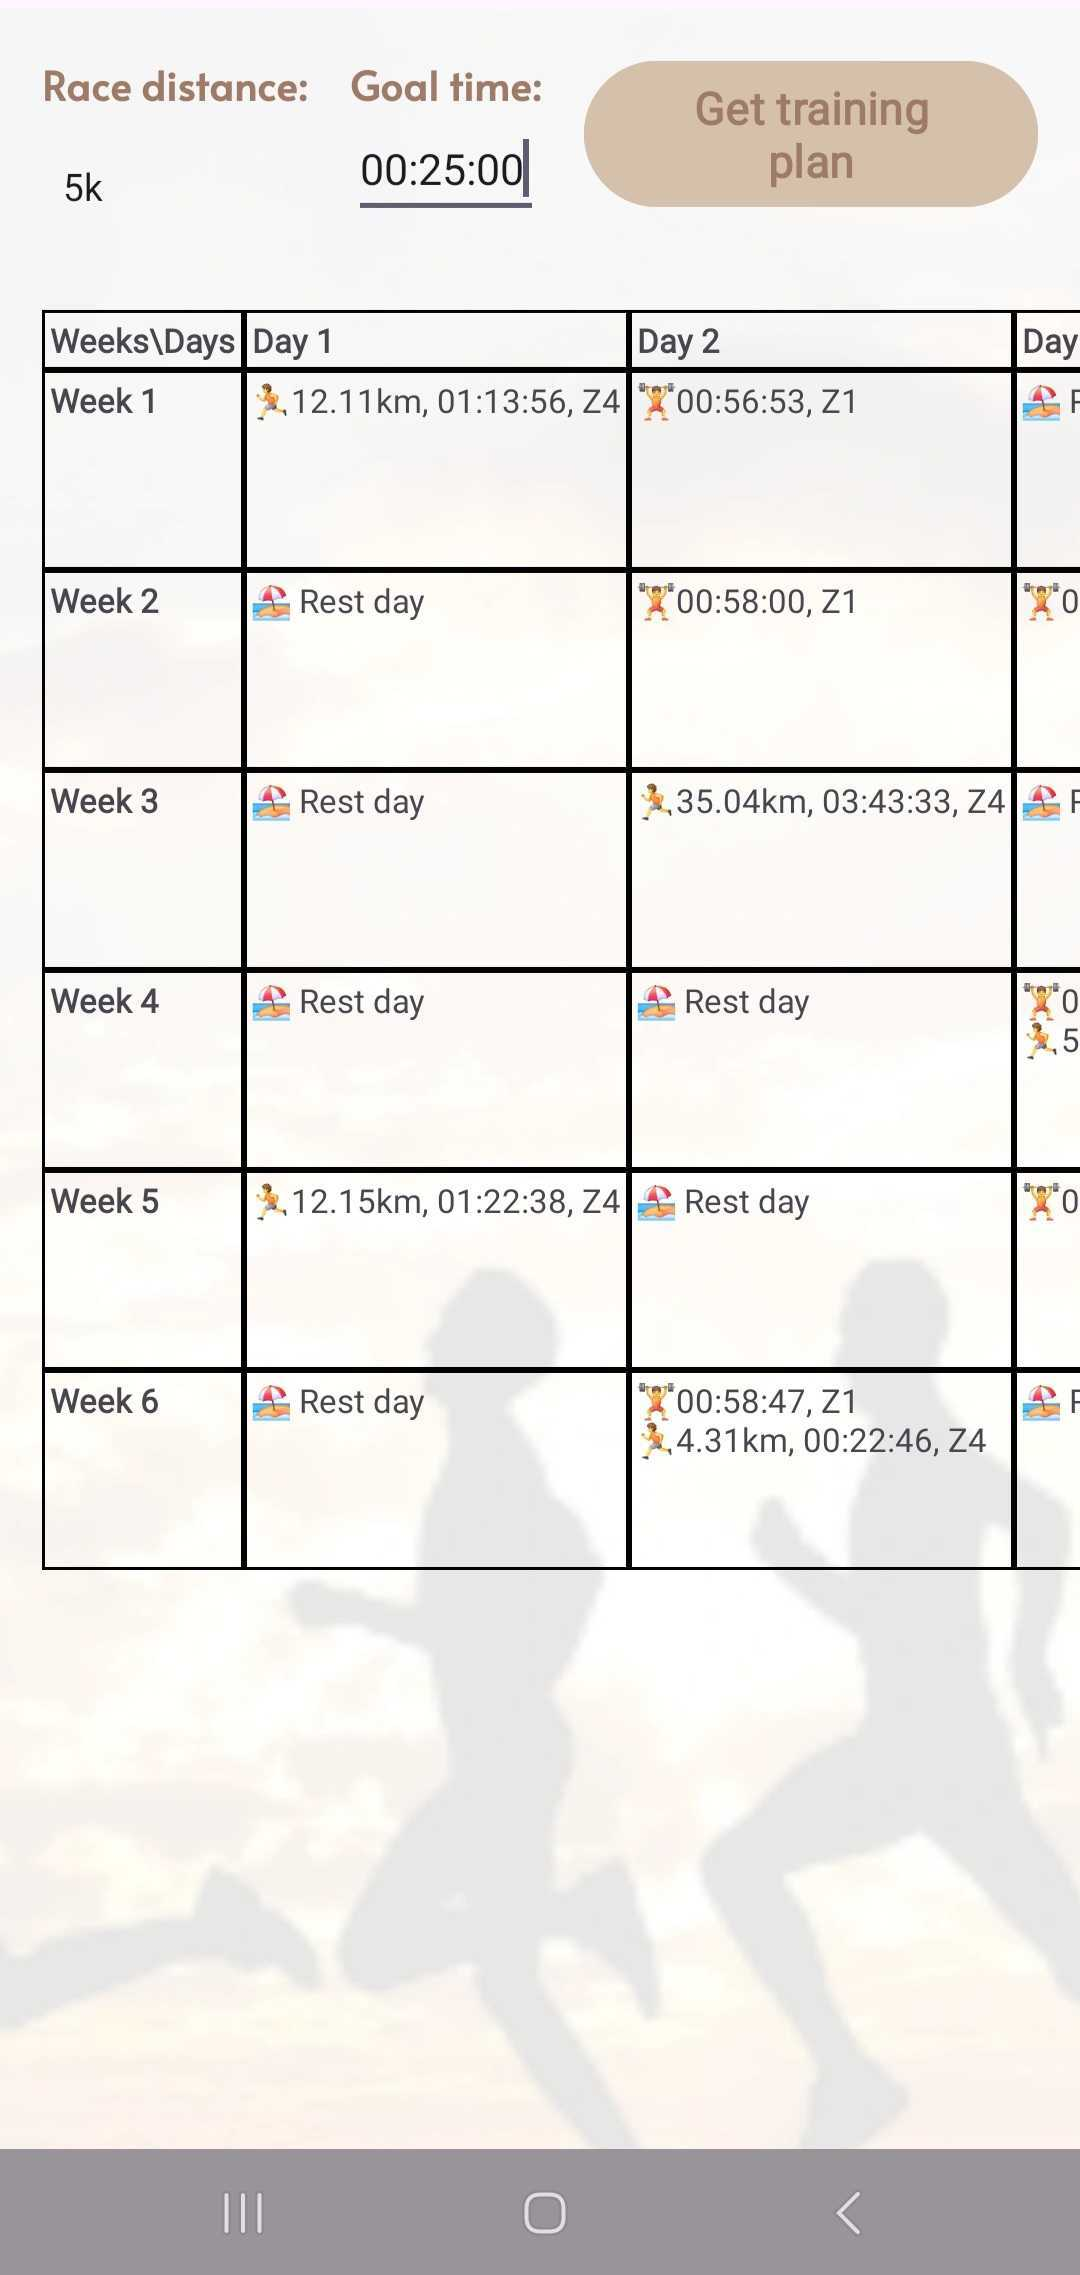
\includegraphics[width=\textwidth]{assets/pictures/app_screenshots/training_plan_1.jpg}
  \end{minipage}
  \hfill
  \begin{minipage}{0.23\textwidth}
    \centering
    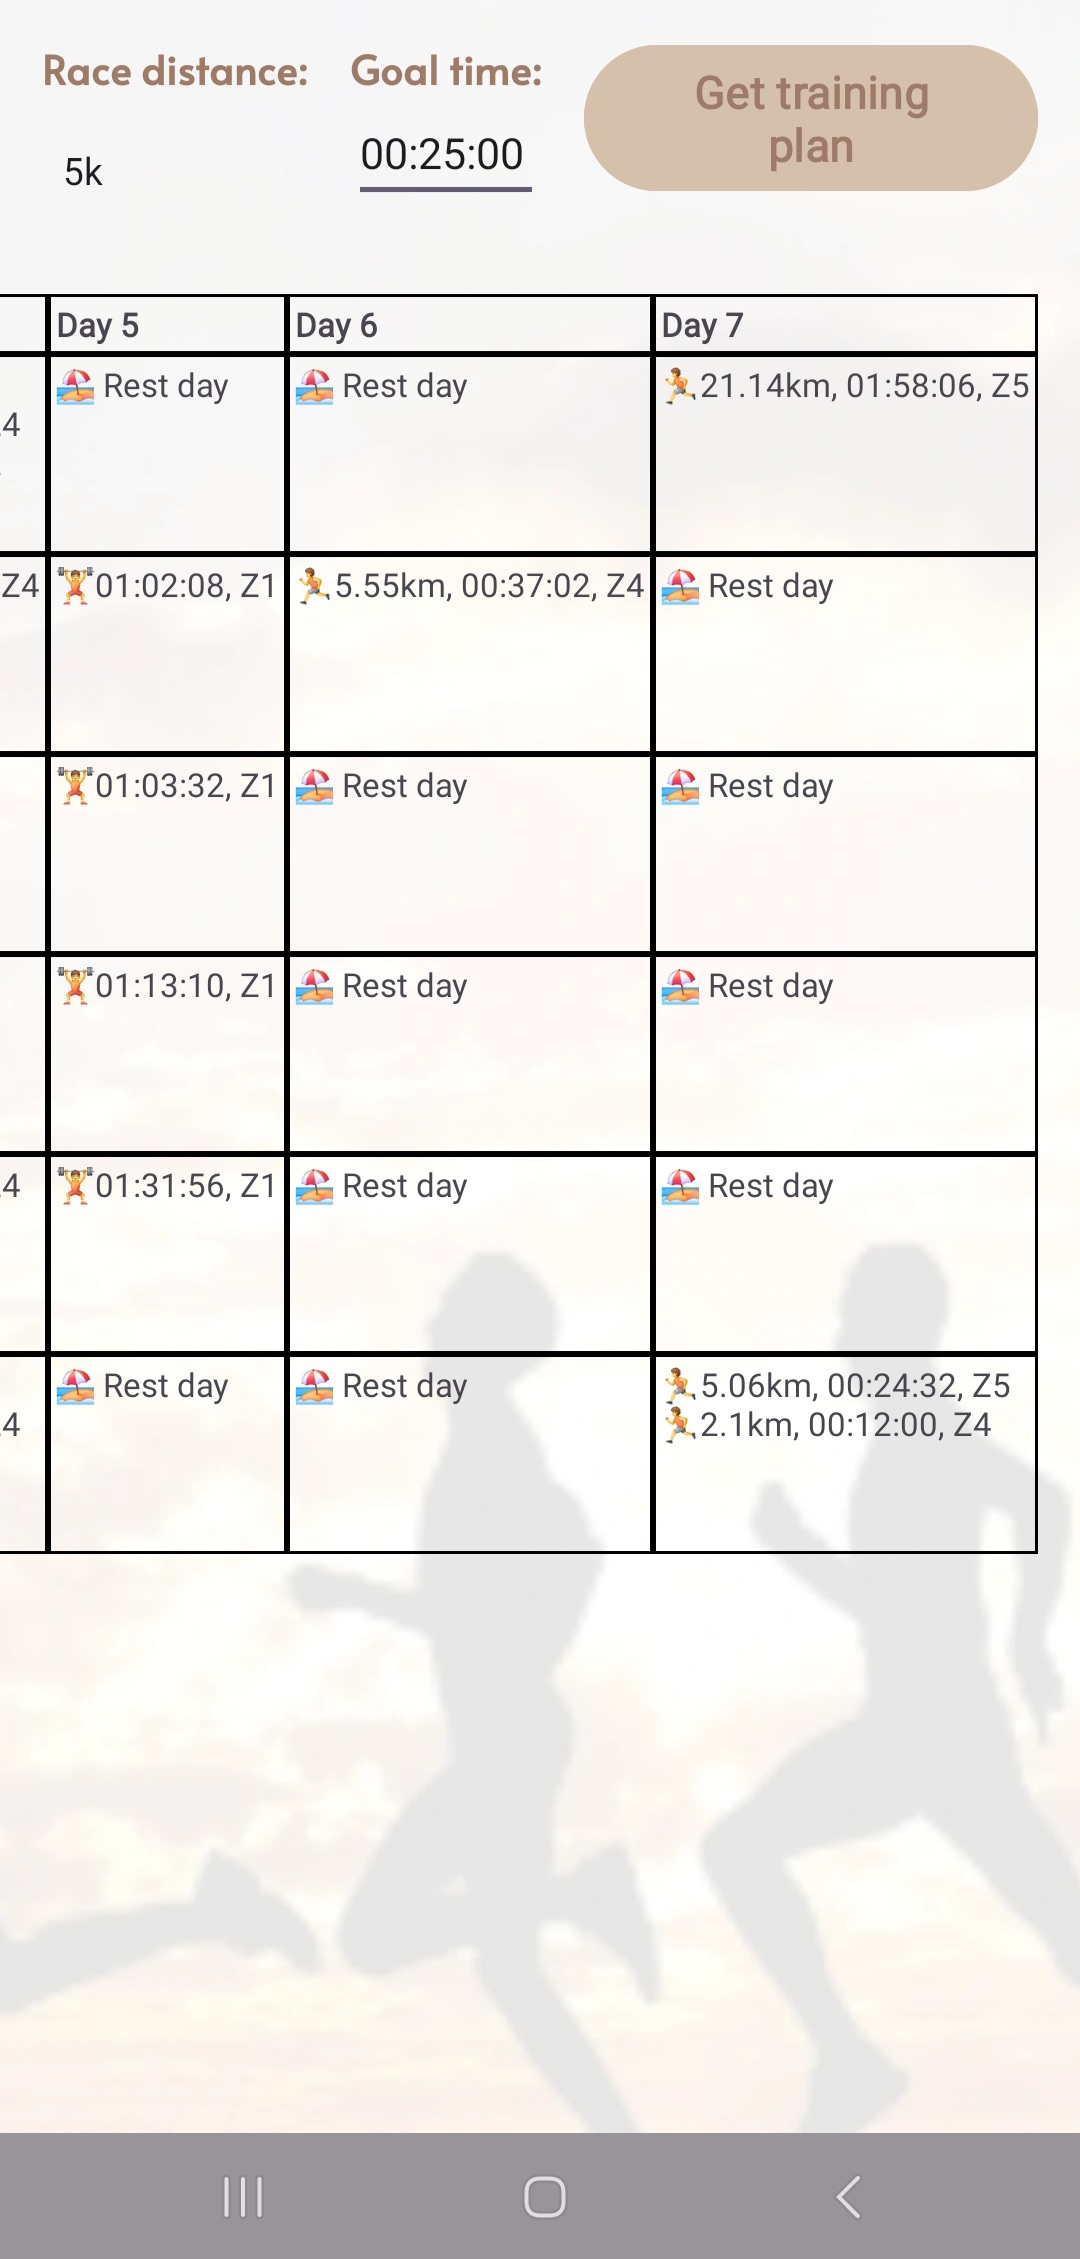
\includegraphics[width=\textwidth]{assets/pictures/app_screenshots/training_plan_2.jpg}
  \end{minipage}
    \hfill
  \begin{minipage}{0.23\textwidth}
    \centering
    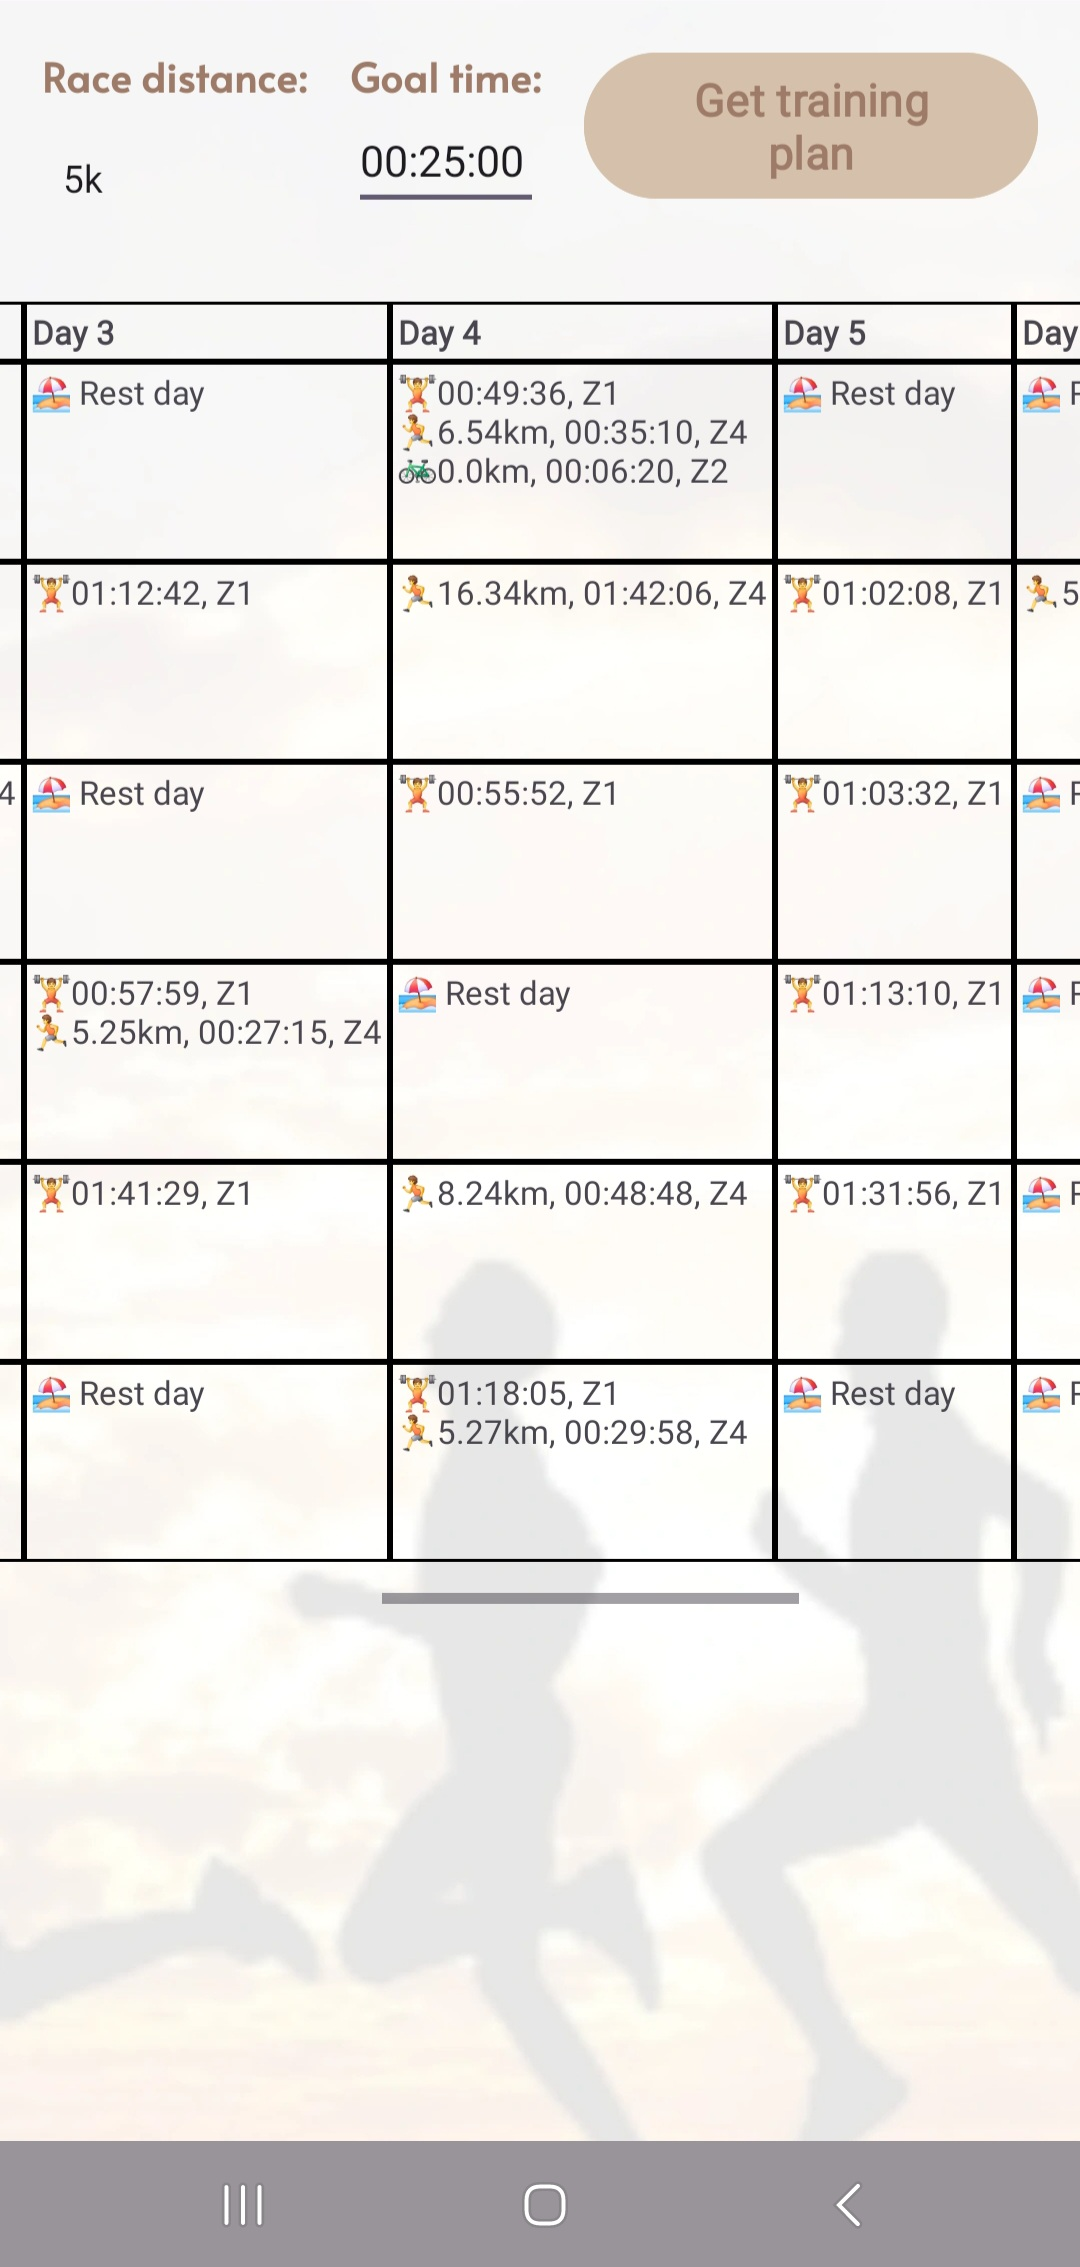
\includegraphics[width=\textwidth]{assets/pictures/app_screenshots/training_plan_3.jpg}
  \end{minipage}
  \caption{Изглед екрана са планом тренинга (хоризонтално померање садржаја табелице са тренингом)}
  \label{pic:training_plan}
\end{figure}


\begin{figure}[h]
  \begin{minipage}{0.45\textwidth}
    \centering
    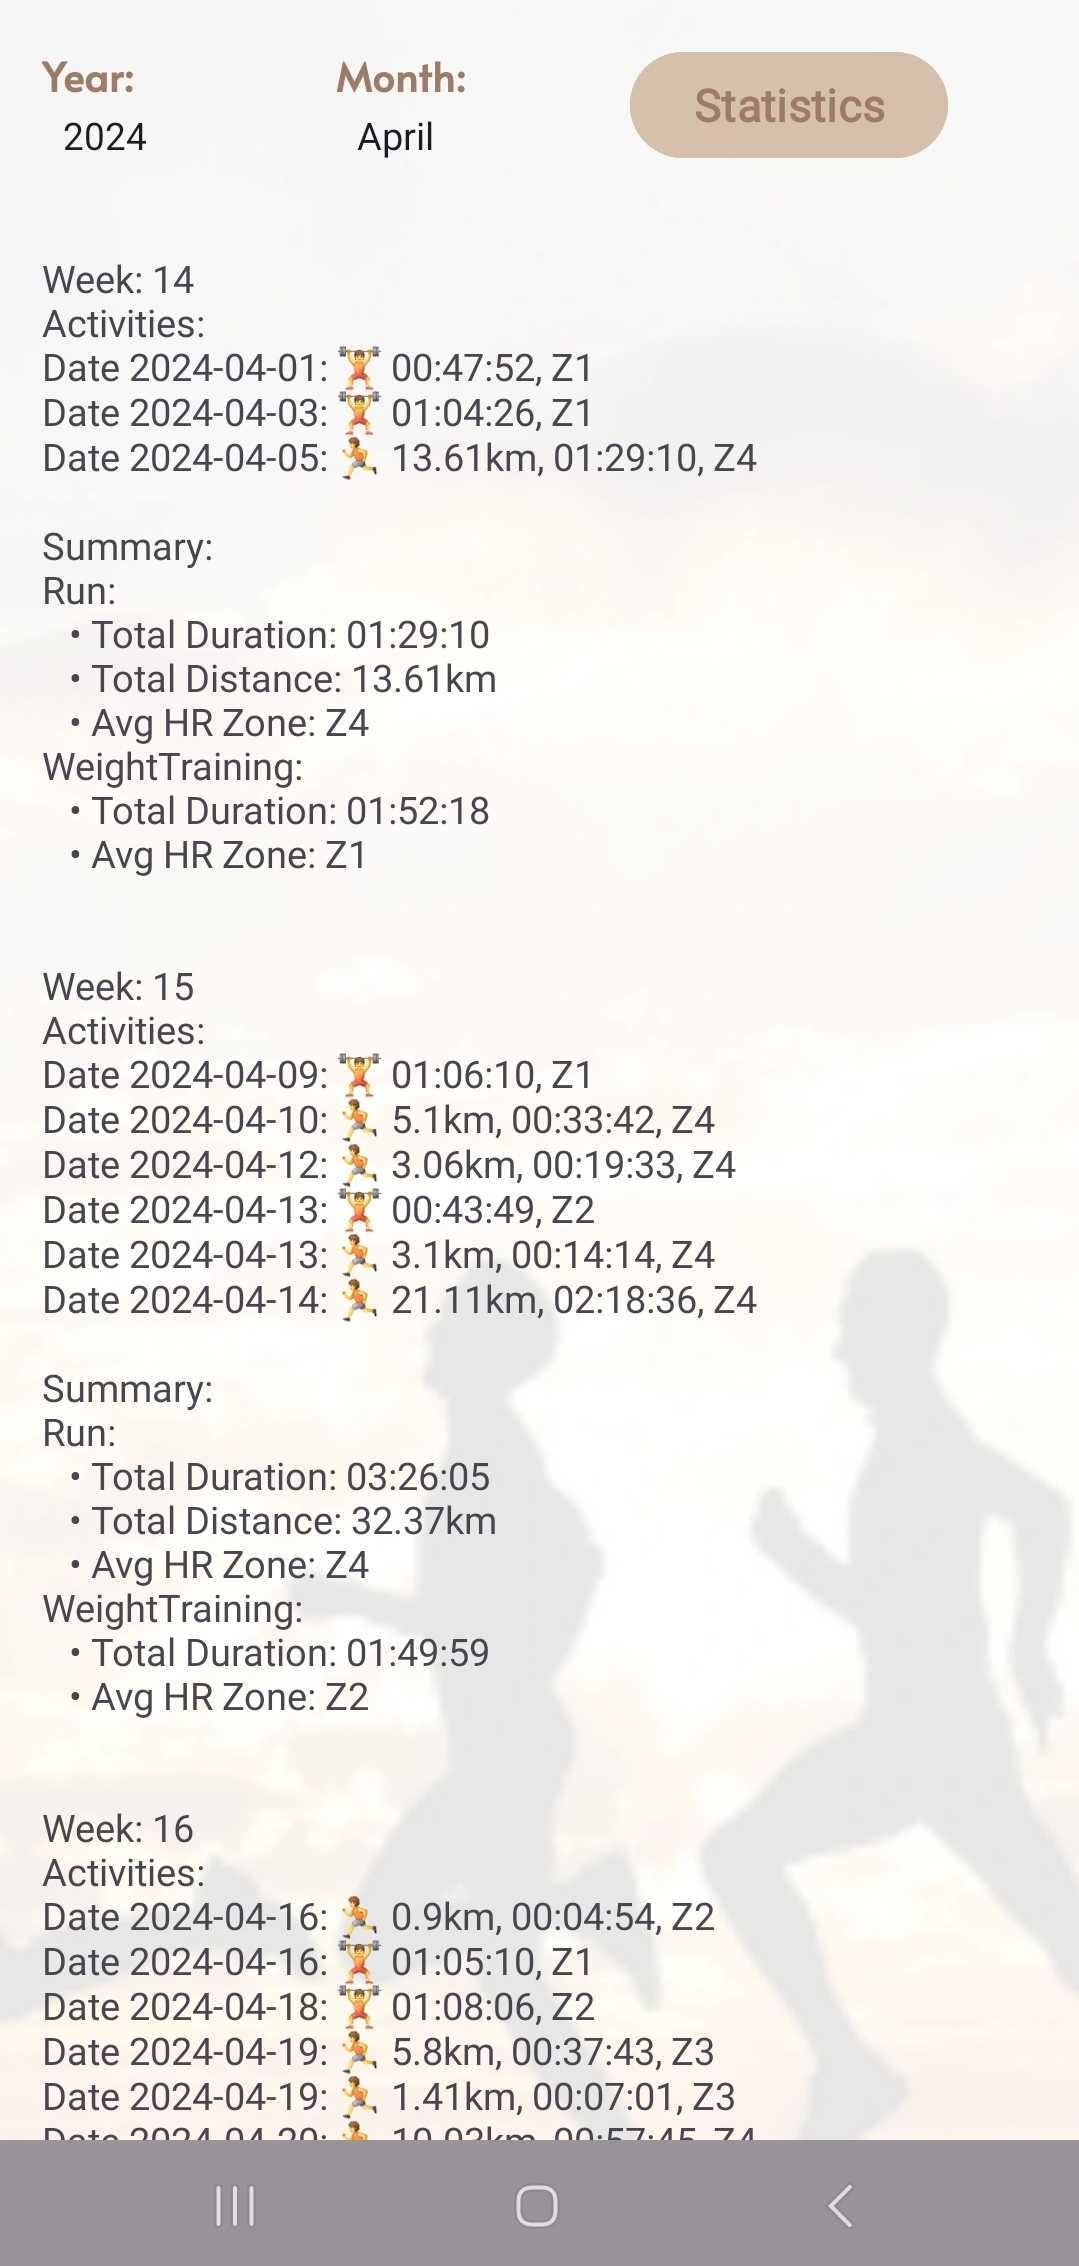
\includegraphics[scale=0.128]{assets/pictures/app_screenshots/training_stats_1.jpg}
  \end{minipage}
  \hfill
  \begin{minipage}{0.45\textwidth}
    \centering
    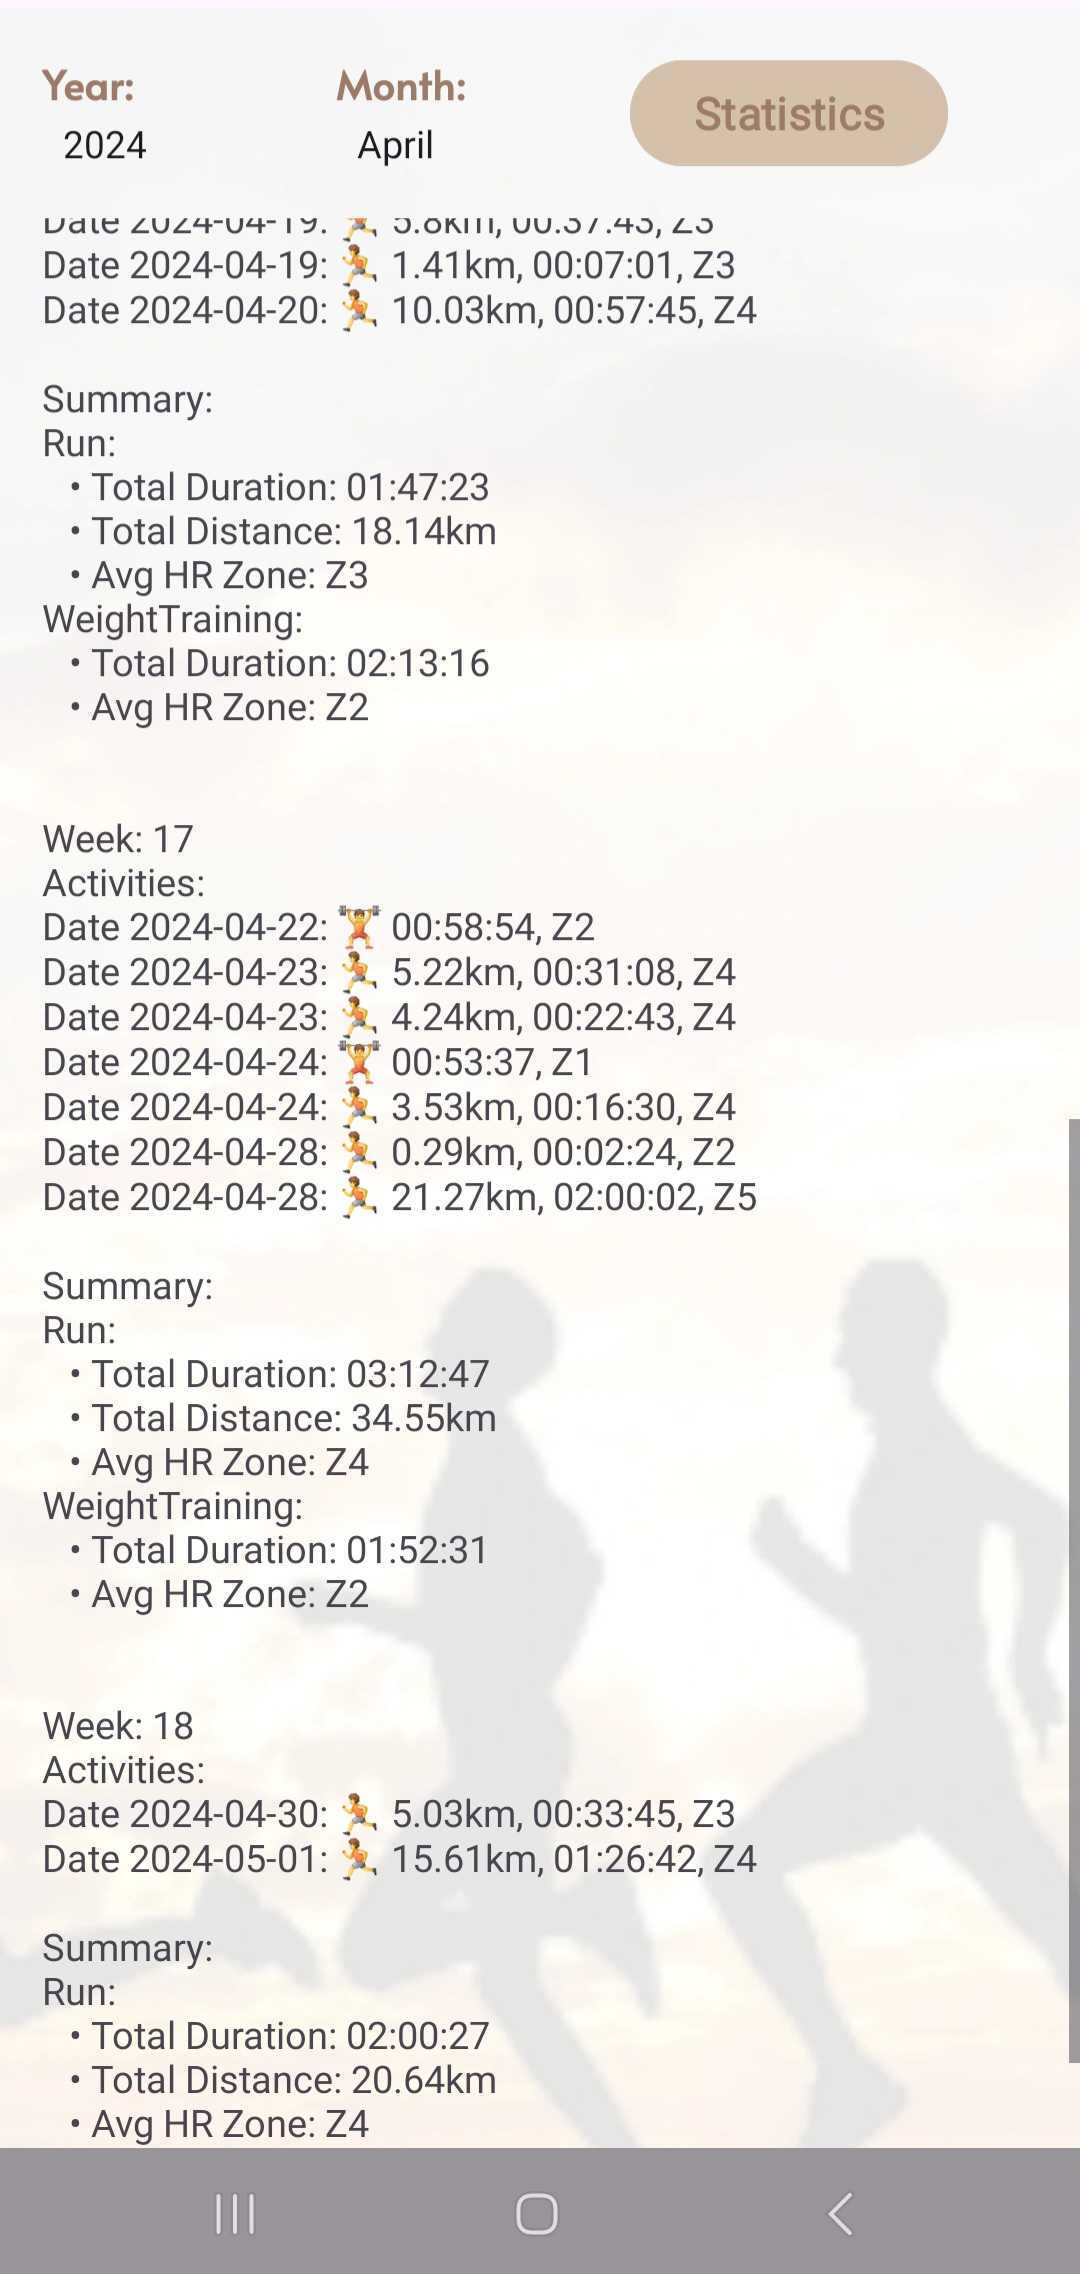
\includegraphics[scale=0.128]{assets/pictures/app_screenshots/training_stats_2.jpg}
  \end{minipage}
  \caption{Изглед месечне статистике тренинга}
  \label{pic:training_stats}
\end{figure}


Поред описаних примарних опција, екран са главним менијем нуди могућност за преусмерење на активност са подацима о налогу корисника кликом на дугме \textit{Profile}, дугме за ауторизацију са апликацијом \textit{Strava} и дугме за одјављивање корисника.

Уколико корисник одлучи да повеже свој налог са налогом на апликацији \textit{Strava}, биће преусмерен на веб сајт за одобрење ауторизације ове апликације. Након тога, клијентска апликација позива захтев за добијање података о кориснику како би проверила да ли се у бази уписао идентификатор ка налогу ове апликације, и уколико јесте, чува га у класи \texttt{ProfileSingleton} како би се након враћања корисника на главни мени приказало да је налог увезан.


Поред прегледа профила, екран за профил корисника (слика \ref{pic:profile}), има опцију за мењање корисничких података и брисање налога. Уколико корисник промени своје податке и сачува промене кликом на дугме \textit{Save changes}, клијентска апликација шаље захтев серверској за промену података, и у случају успешног одговора, ажурира атрибуте класе \texttt{ProfileSingleton} у складу са променама. Подаци из ове класе, као и токени за приступ серверској апликацији се бришу у случају да корисник одлучи да обрише свој налог или да се одјави са апликације. У случају одјављивање се додатно шаље захтев за опозивање токена ка серверској страни апликације. У оба случаја, корисник ће након слања захтева серверској апликацији бити преусмерен на екран за пријаву на апликацију.

\begin{figure}[h]
  \centering
  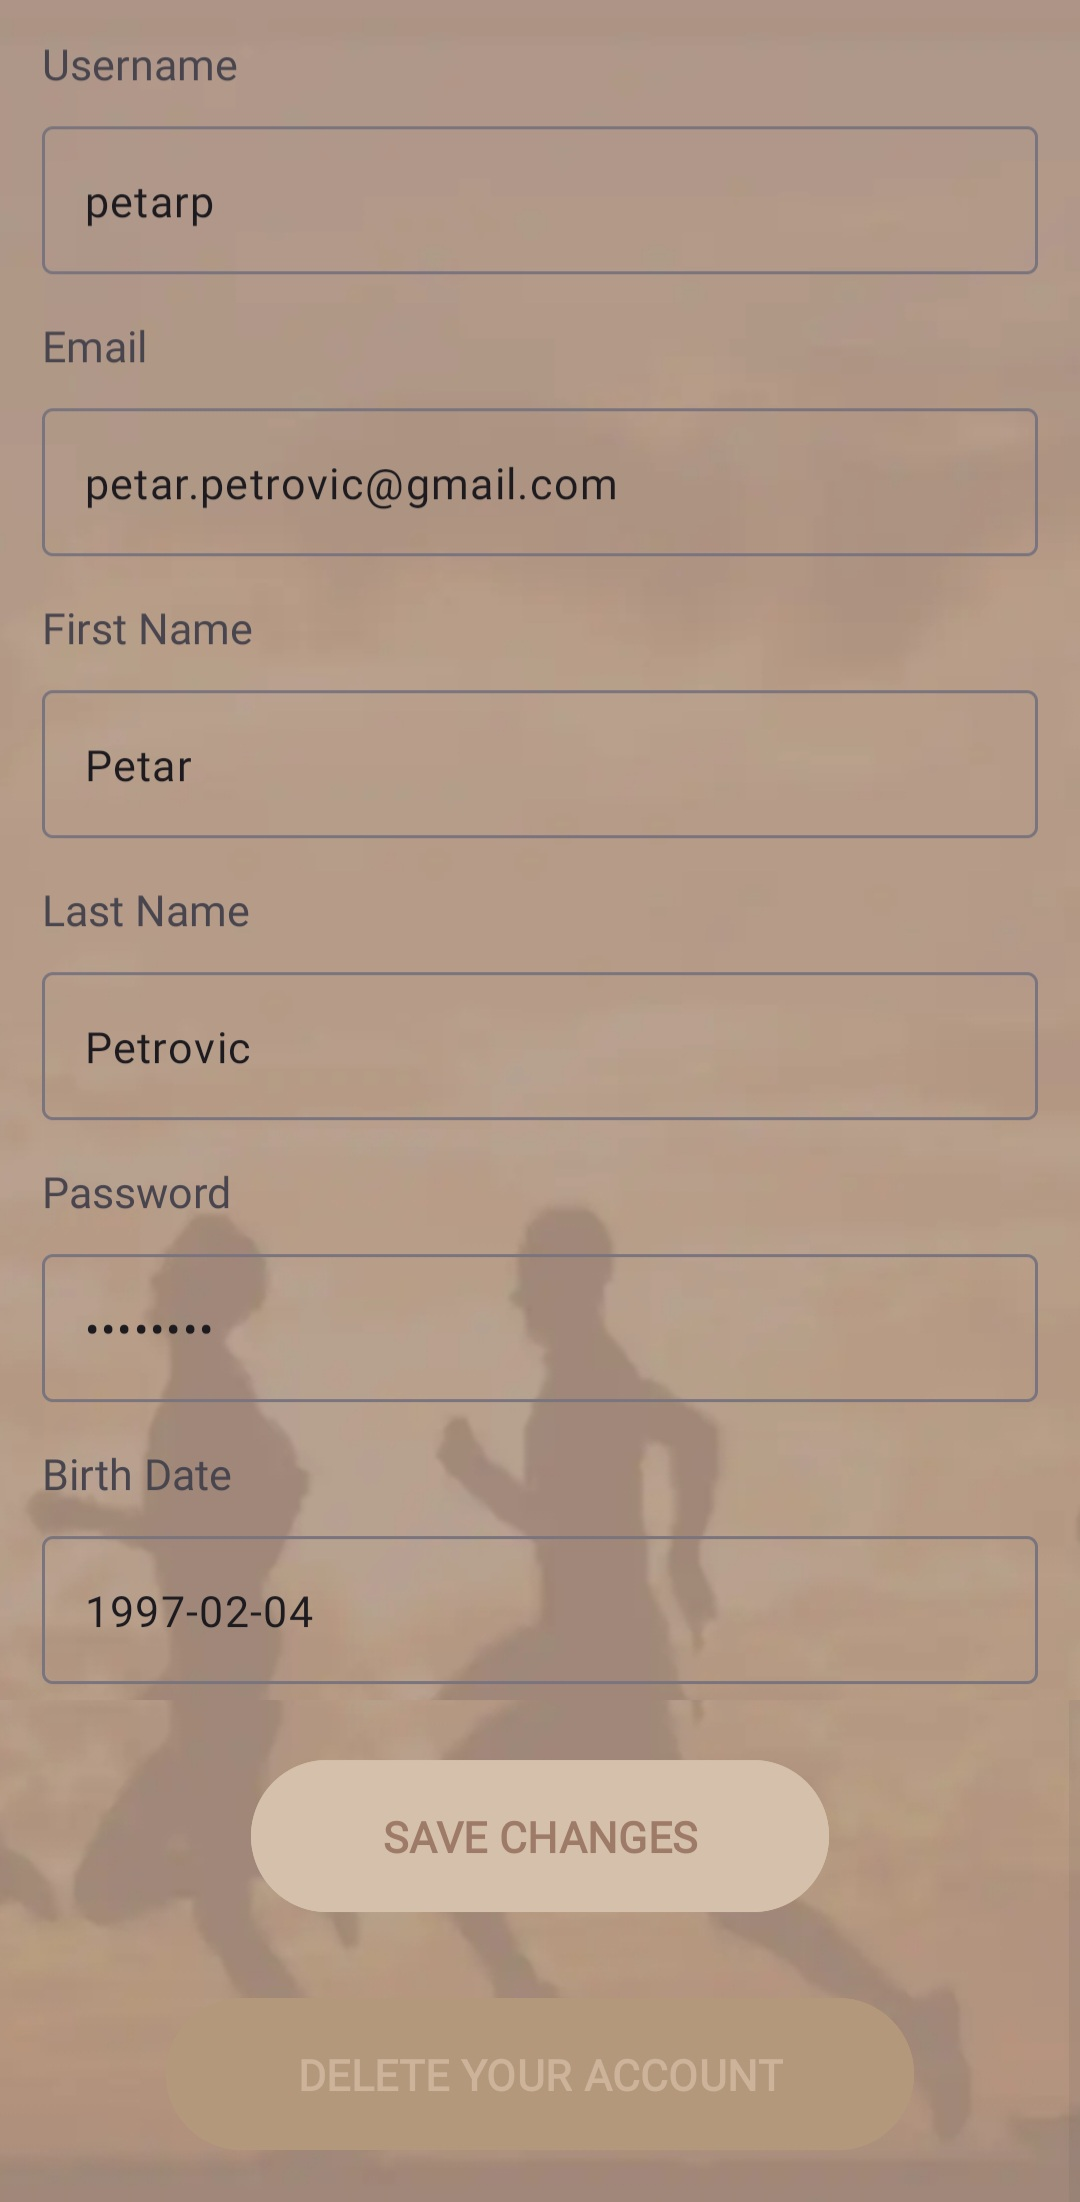
\includegraphics[scale=0.1]{assets/pictures/app_screenshots/profile.jpg}
    \caption{Приказ профила корисника апликације \textit{Train Wiser}}
  \label{pic:profile}
\end{figure}

\section{Случајеви употребе}


У овом потпоглављу је детаљно изложено како се апликација \textit{Train Wiser} користи кроз токове случајева употребе. Уколико дође до грешке при раду апликације, грешка ће бити приказана као \textit{Toast} порука на дну екрана. Приликом финалног тестирања апликације, интерне грешке на серверској страни се нису јављале. Како би се демонстрирали алтернативни токови за случај интерне грешке на серверу, симулирана је намерна грешка на серверској страни и приказана на слици \ref{pic:error-500}. Такође, у току финалног тестирања апликације није долазило до неауторизованих захтева са клијентске стране, симулација грешке је приказана на слици \ref{pic:error-401}.\footnote{Интерне грешке на серверској страни апликације и неаутризовани захтеви од стране клијентске су обрађене на исти начин на нивоу клијентске апликације, на приказаним примерима је илустрован случај са активношћу за генерисање плана тренинга} Ради веће прегледности, приказ генералних грешака поменутих типова приликом захтева је изостављен на илустрацијама случајева употребе.

\begin{figure}[H]
  \centering
  \begin{minipage}{0.45\textwidth}
    \centering
  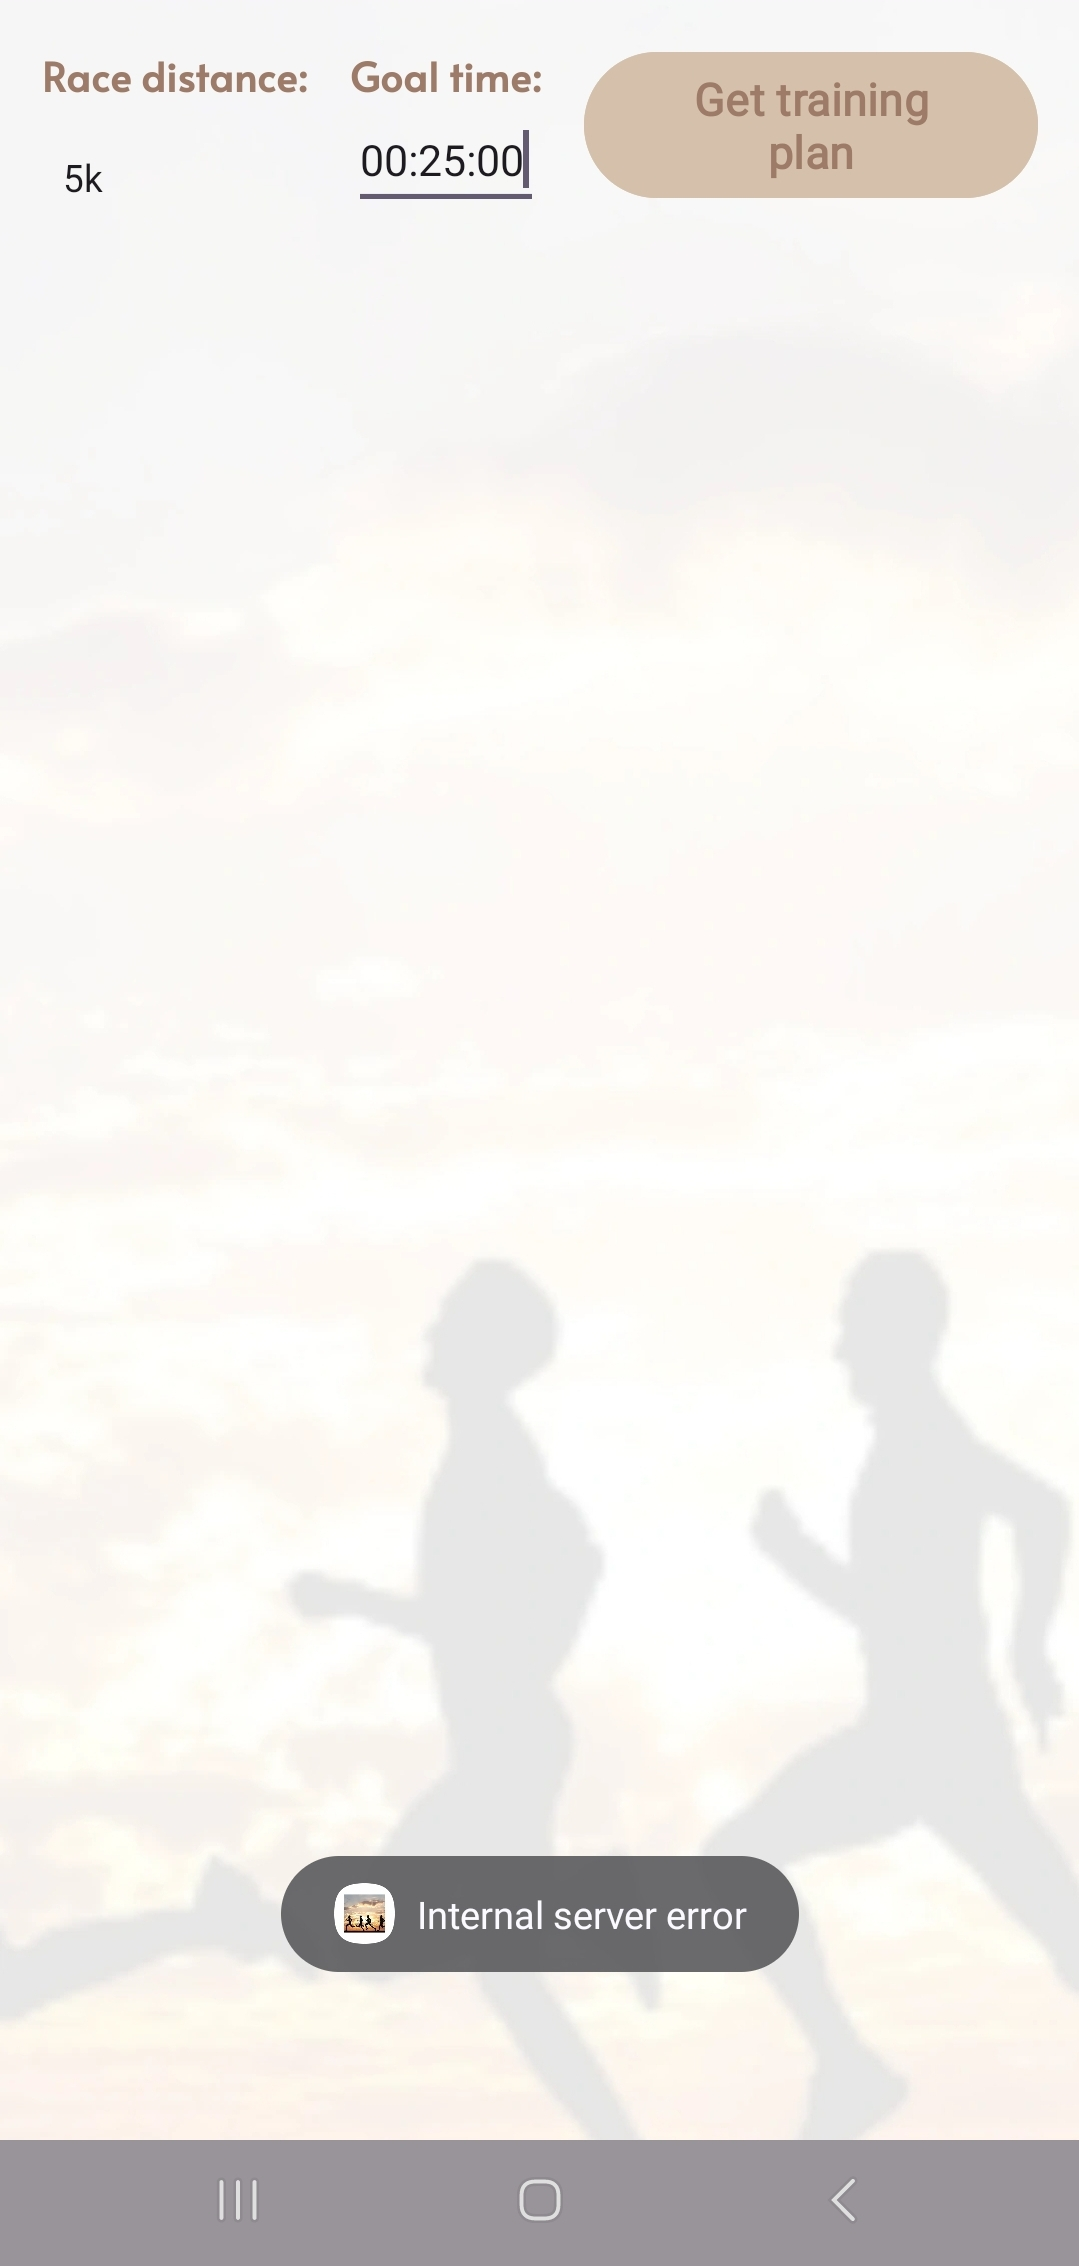
\includegraphics[scale=0.14]{assets/pictures/errors/500_server_error.jpg}
    \caption{Приказ симулиране интерне грешке на серверској страни апликације \textit{Train Wiser}}
  \label{pic:error-500}
  \end{minipage}
  \hfill
  \begin{minipage}{0.45\textwidth}
    \centering
  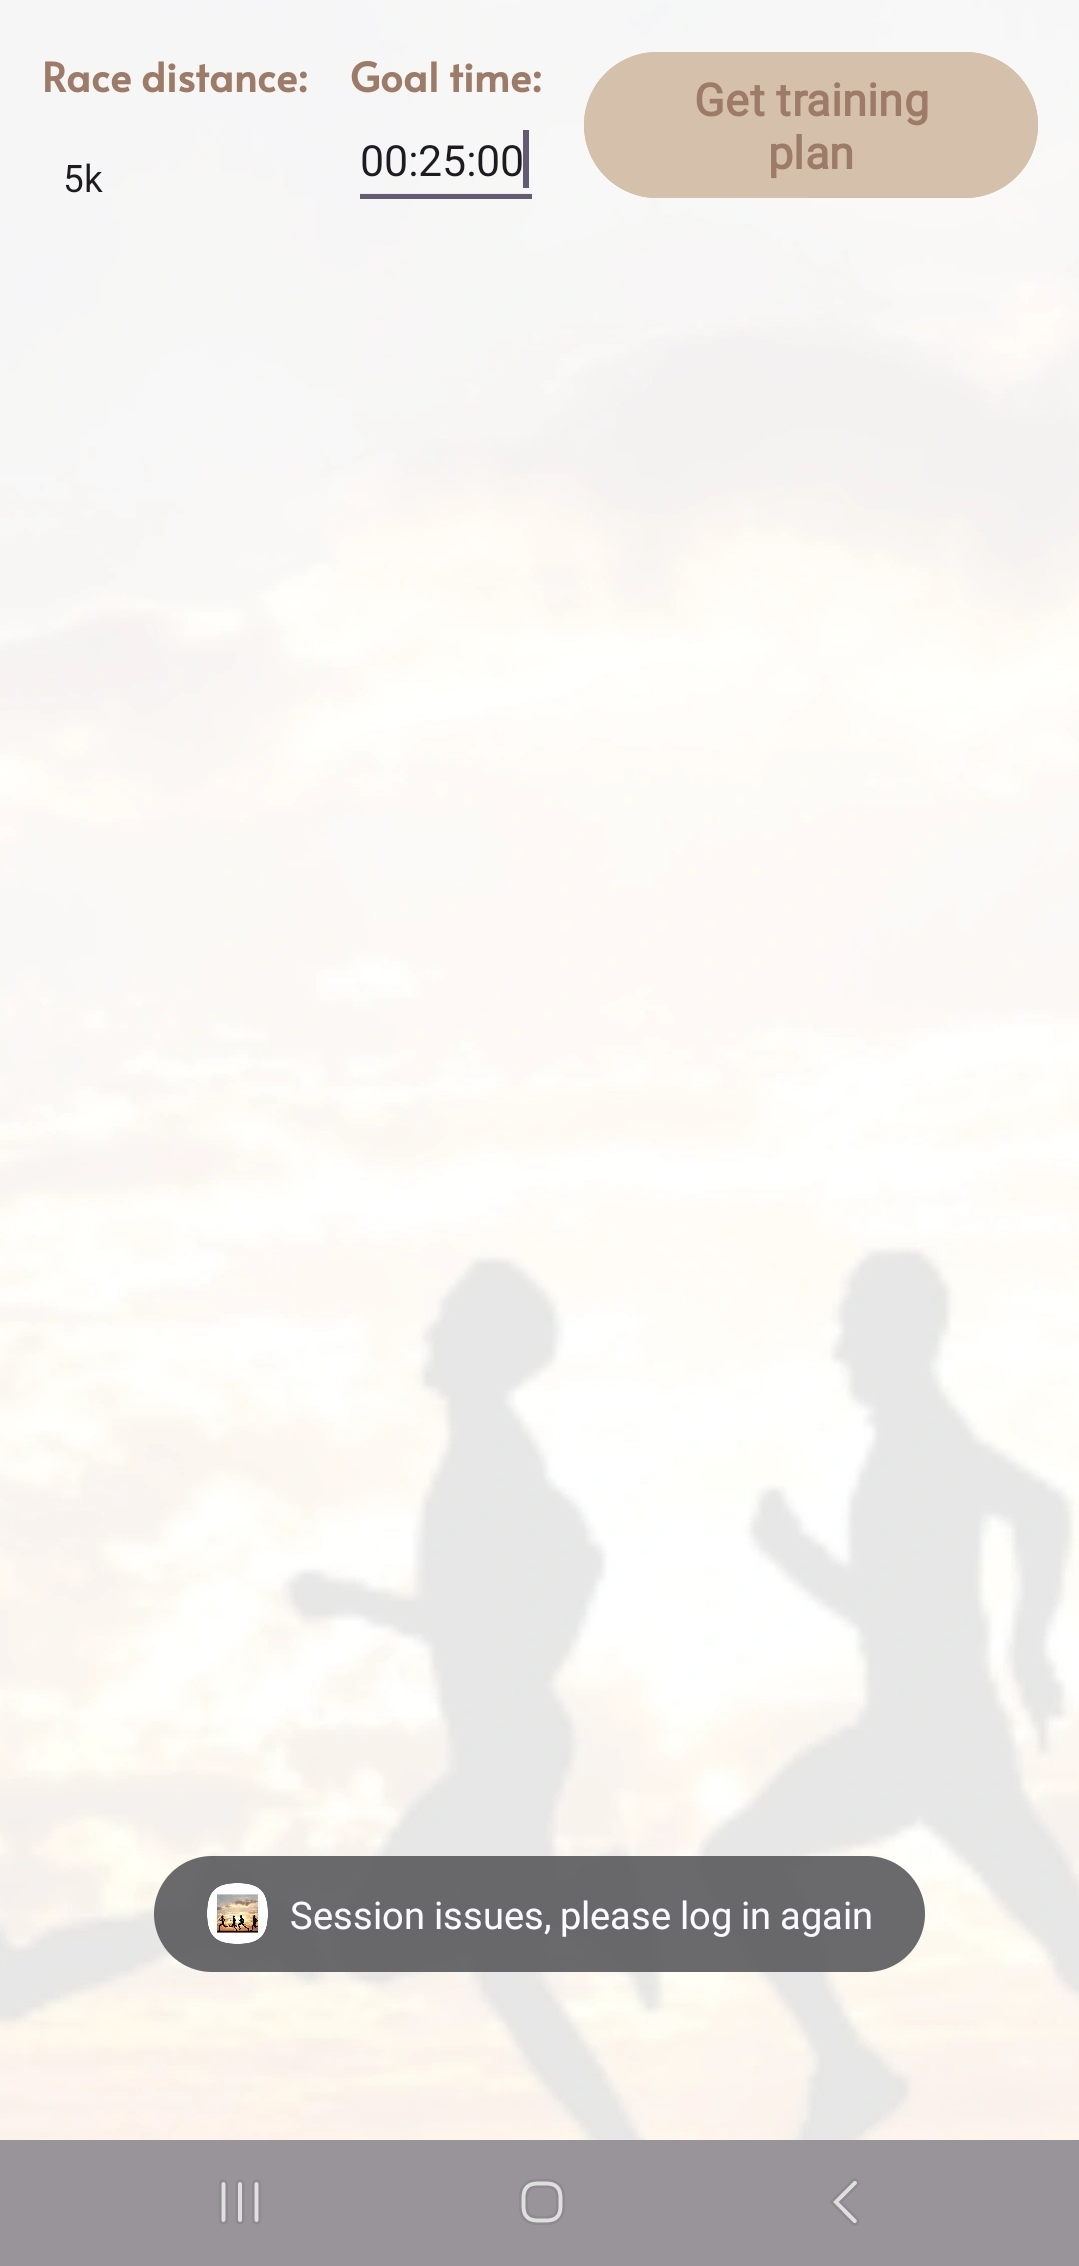
\includegraphics[scale=0.131]{assets/pictures/errors/server_401_error.jpg}
    \caption{Приказ симулиране грешке приликом неауторизованог захтева са клијентске стране апликације \textit{Train Wiser}}
  \label{pic:error-401}
  \end{minipage}
\end{figure}

\subsection*{Регистрација корисника}
\begin{longtable}{p{0.23\linewidth} p{0.77\linewidth}}
 \hline
 \textit{\textbf{Актери}} & Корисник, систем (клијентска и серверска апликација) \\
\hline
\textit{\textbf{Предуслови}} & Корисник нема налог за апликацију \\
 \hline
\textit{\textbf{Постуслови}} & Корисник је регистровао свој налог за апликацију \\
 \hline
 \textit{\textbf{Главни ток}} &  
    \begin{enumerate}
        \item Корисник на екрану за пријављивање на апликацију бира опцију за преусмерење на регистрацију кликом на одговарајућу лабелу
        \item Корисник попуњава сва потребна поља и притиска дугме \textit{SIGN UP} 
        \item Клијентска апликација шаље захтев за регистрацију новог корисника серверској
        \item Серверска апликација чува податке о кориснику у бази
        \item Клијентска апликација преусмерава корисника на екран за пријављивање
    \end{enumerate}\\
 \hline
\textit{\textbf{Алтернативни ток 1}} & Уколико садржај поља за унос није прошао валидацију, корисник се обавештава о грешци и случај употребе се наставља у тачки 2.\\
 \hline
\textit{\textbf{Алтернативни ток 2}} & Уколико је приликом захтева настала грешка која није везана за невалидност унетих параметара, корисник се обавештава о грешци и случај употребе се завршава \\
 \hline
\end{longtable} 

\noindent Ток случаја употребе је приказан на слици \ref{pic:registration-flow}.

\begin{figure}[H]
  \centering
  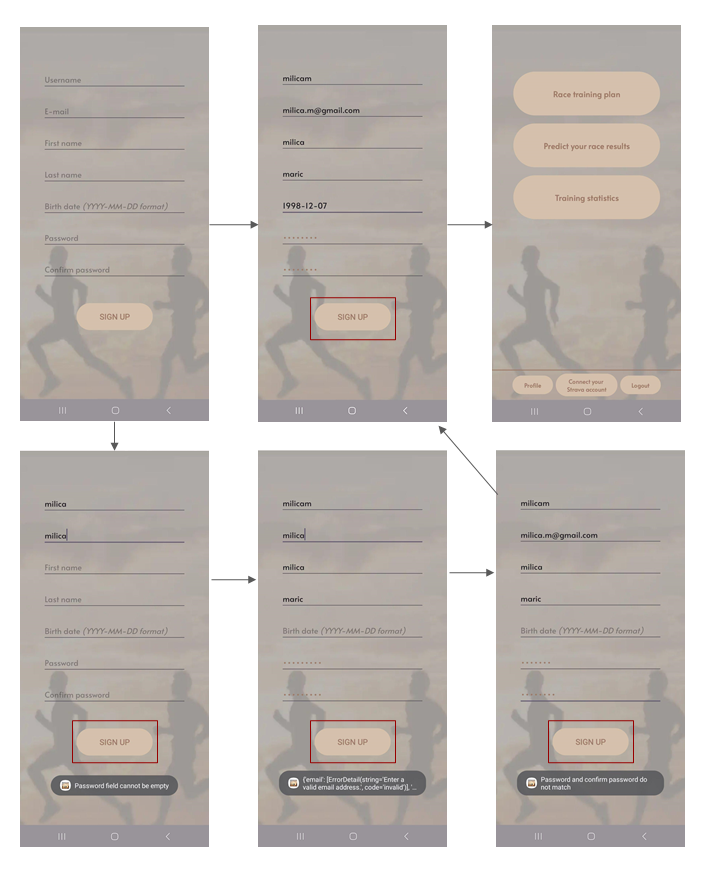
\includegraphics[scale=0.85]{assets/pictures/usecases_flows/signup_flow.png}
    \caption{Приказ тока случаја употребе за регистрацију корисника}
  \label{pic:registration-flow}
\end{figure}

%%%%%

\newpage
\subsection*{Пријављивање корисника}


\begin{longtable}{p{0.23\linewidth} p{0.77\linewidth}}
 \hline
 \textit{\textbf{Актери}} & Корисник, систем (клијентска и серверска апликација) \\
\hline

\textit{\textbf{Предуслови}} & Корисник нема сачуване токене за приступ серверској апликацији на уређају, тј. није пријављен на апликацију \\
 \hline
\textit{\textbf{Постуслови}} & Кориснички је пријављен на апликацију \\
 \hline
 \textit{\textbf{Главни ток}} &  
    \begin{enumerate}
        \item Будући да корисник није пријављен, након уласка у апликацију, систем га преусмерава на екран за пријаву 
        \item Корисник попуњава сва потребна поља и притиска дугме \textit{LOG IN} 
        \item Клијентска апликација шаље захтев серверској за пријаву корисника 
        \item Серверска апликација узвраћа токене за пријаву
        \item Клијентска апликација чува токене
        \item Клијентска апликација преусмерава корисника на екран са главним менијем
    \end{enumerate}\\
 \hline
\textit{\textbf{Алтернативни ток 1}} & Уколико је корисник унео невалидне податке за аутентификацију, систем га обавештава о грешци и случај употребе се завршава \\
 \hline
\textit{\textbf{Алтернативни ток 2}} & Уколико је настала грешка приликом захтева, корисник се обавештава о грешци и случај употребе се завршава \\
 \hline
\end{longtable}

\noindent Ток случаја употребе је приказан на слици \ref{pic:login-flow}.

\begin{figure}[H]
  \centering
  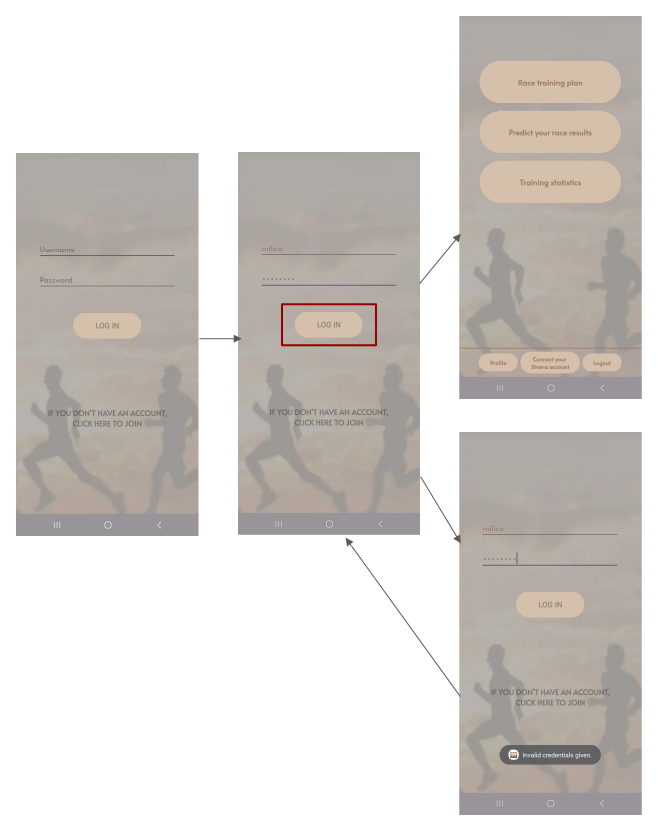
\includegraphics[scale=0.9]{assets/pictures/usecases_flows/login_flow.png}
    \caption{Приказ тока случаја употребе за пријављивање корисника}
  \label{pic:login-flow}
\end{figure}


%%%%%%%
\newpage

\subsection*{Одјављивање корисника}

\begin{longtable}{p{0.23\linewidth} p{0.77\linewidth}}
 % Akteri
 \hline
 \textit{\textbf{Актери}} & Корисник, систем (клијентска и серверска апликација) \\
\hline

\textit{\textbf{Предуслови}} & Корисник је пријављен на апликацију \\
 \hline


\textit{\textbf{Постуслови}} & Корисник је одјављен са апликације \\
 \hline
 \textit{\textbf{Главни ток}} &  
    \begin{enumerate}
        \item Уколико корисник није на главном менију, корисник се пребацује на главни мени
        \item Корисник притиска дугме \textit{Logout} за одјављивање
        \item Систем позива захтев за опозивање приступног токена
        \item Систем брише токене за приступ серверској апликацији са уређаја корисника
        \item Систем преусмерава корисника на екран за пријављивање на апликацију
    \end{enumerate}\\
 \hline

\textit{\textbf{Алтернативни ток}} & Уколико се десила грешка приликом захтева за опозивање токена, случај употребе се наставља у тачки 4., а корисник приликом следеће пријаве добија нови приступни токен \\
 \hline
 
\end{longtable}

%%%%%%

\subsection*{Ажурирање корисничких података}
\begin{longtable}{p{0.23\linewidth} p{0.77\linewidth}}

 \hline
 \textit{\textbf{Актери}} & Корисник, систем (клијентска и серверска апликација) \\
\hline

\textit{\textbf{Предуслови}} & Корисник је пријављен на апликацију \\
 \hline
\textit{\textbf{Постуслови}} & Корисник је ажурирао жељене податке о свом профилу \\
 \hline
 \textit{\textbf{Главни ток}} & 
    \begin{enumerate}
        \item Уколико корисник није на главном менију, корисник се позиционира на главни мени
        \item Корисник бира опцију за преглед профила кликом на дугме \textit{Profile}
        \item Корисник мења све приказане податке свог профила које жели да промени
        \item Корисник притиска дугме \textit{SAVE CHANGES} за чување промена
        \item Систем проверава која поља су ажурирана и шаље захтев са промењеним параметрима профила
        \item Систем обавештава корисника да су промене профила успешно сачуване
        \item Систем преусмерава корисника на главни мени
    \end{enumerate}\\
 \hline
\textit{\textbf{Алтернативни ток 1}} & Уколико садржај поља за унос није прошао валидацију, корисник се обавештава о грешци и случај употребе се наставља у тачки 2.\\
 \hline
\textit{\textbf{Алтернативни ток 2}} & Уколико је приликом захтева настала грешка која није везана за невалидност унетих параметара, корисник се обавештава о грешци и случај употребе се завршава \\
 \hline 
\end{longtable}

Изглед овог тока случаја употребе је сличан току за регистрацију корисника, будући да су грешке које могу настати при попуњавању поља исте као за регистрацију.

%%%%%


\subsection*{Брисање налога}
\begin{longtable}{p{0.23\linewidth} p{0.77\linewidth}}
 \hline
 \textit{\textbf{Актери}} & Корисник, систем (клијентска и серверска апликација) \\
\hline

\textit{\textbf{Предуслови}} & Корисник је пријављен на апликацију \\
 \hline
\textit{\textbf{Постуслови}} & Корисник је обрисао налог за апликацију \\
 \hline
 \textit{\textbf{Главни ток}} &  
    \begin{enumerate}
        \item Уколико корисник није на главном менију, корисник се пребацује на главни мени
        \item Корисник бира опцију за преглед профила кликом на дугме \textit{Profile}
        \item Корисник притиска дугме \textit{DELETE YOUR ACCOUNT} за брисање налога
        \item Клијентска апликација позива захтев за брисање налога на серверској апликацији
        \item Клијентска апликација брише токене за приступ серверској апликацији са уређаја корисника
        \item Систем преусмерава корисника на екран за пријављивање на апликацију
    \end{enumerate}\\
 \hline

\textit{\textbf{Алтернативни ток}} & Уколико се десила грешка приликом захтева за брисање налога, систем обавештава корисника о грешци и случај употребе се наставља у тачки 5. \\
 \hline
\end{longtable}

Ток случаја употребе је приказан на слици \ref{pic:delete-account-flow}.

\begin{figure}[H]
  \centering
  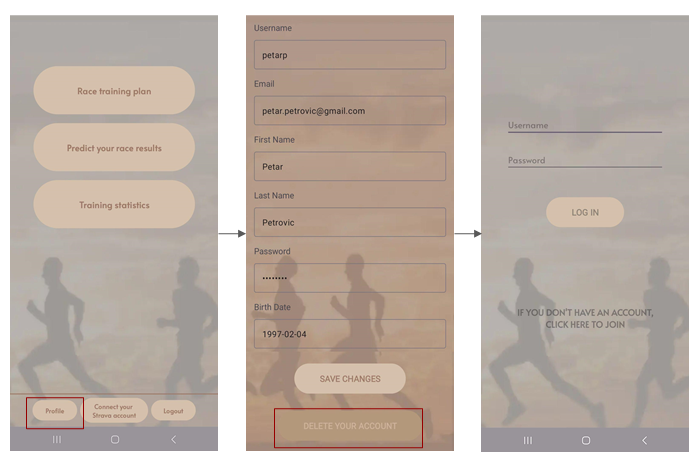
\includegraphics[scale=0.9]{assets/pictures/usecases_flows/delete_account_flow.png}
    \caption{Приказ тока случаја употребе за брисање корисничког налога}
  \label{pic:delete-account-flow}
\end{figure}

\newpage
\subsection*{Ауторизација налога апликације \textit{Train Wiser} са спољним налогом апликације \textit{Strava}}
\begin{longtable}{p{0.23\linewidth} p{0.77\linewidth}}
 \hline
 \textit{\textbf{Актери}} & Корисник, систем (клијентска и серверска апликација) \\
\hline
\textit{\textbf{Предуслови}} & Корисник је пријављен на апликацију и нема повезан налог са апликацијом \textit{Strava} \\
 \hline
\textit{\textbf{Постуслови}} & Корисник је ауторизовао свој налог са апликације \textit{Train Wiser} на апликацији \textit{Strava} \\
 \hline
 \textit{\textbf{Главни ток}} &  
    \begin{enumerate}
        \item Уколико корисник није на главном менију, корисник се пребацује на главни мени
        \item Корисник бира опцију за повезивање са апликацијом \textit{Strava} кликом на дугме \textit{Connect your Strava account}
        \item Систем преусмерава корисника на страницу апликације \textit{Strava} (на веб прегледачу) за ауторизацију апликације \textit{Train Wiser}
        \item Систем уписује податке о ауторизацији и за највише сат времена покреће преузимање активности корисника
        \item Корисник враћа апликацију \textit{Train Wiser} у први план
        \item Систем онемогућава клик на дугме за конекцију са апликацијом \textit{Strava}
    \end{enumerate}\\
 \hline
\textit{\textbf{Алтернативни ток 1}} & Уколико корисник у тачки 3. није одобрио потребне дозволе апликацији \textit{Train Wiser} или је отказао ауторизацију, добиће одговарајућу поруку са грешком на веб прегледачу и случај употребе се завршава \\
 \hline
\textit{\textbf{Алтернативни ток 2}} & Уколико је приликом захтева настала грешка, корисник се обавештава о грешци и случај употребе се завршава \\
 \hline
\end{longtable}

Ток случаја употребе је приказан на слици \ref{pic:strava-auth-flow}.

\begin{figure}[H]
  \centering
  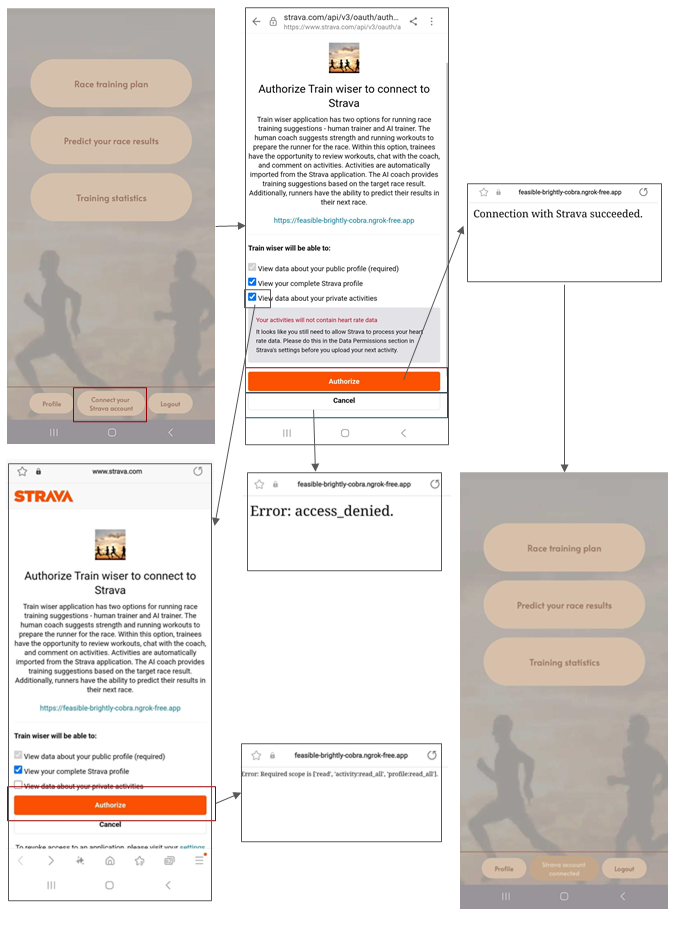
\includegraphics[scale=0.85]{assets/pictures/usecases_flows/strava_auth_flow.png}
    \caption{Приказ тока случаја употребе за ауторизацију са спољним налогом апликације \textit{Strava}}
  \label{pic:strava-auth-flow}
\end{figure}


%%%%%%%
\newpage
\subsection*{Предлагање планова тренинга за остваривање одређених резултата}
\begin{longtable}{p{0.23\linewidth} p{0.77\linewidth}}
 \hline
 \textit{\textbf{Актери}} & Корисник, систем (клијентска и серверска апликација) \\
\hline

\textit{\textbf{Предуслови}} & Корисник је пријављен на апликацију \\
 \hline

\textit{\textbf{Постуслови}} & Корисник је добио до највише пет планова тренинга за одређену дистанцу и циљно време \\
 \hline
 \textit{\textbf{Главни ток}} &  
    \begin{enumerate}
        \item Корисник са главног менија бира опцију за израду плана тренинга кликом на дугме \textit{Race training plan}
        \item Корисник бира дистанцу и циљно време
        \item Корисник притиска дугме \textit{Get training plan} за генерисање планова тренинга
        \item Клијентска апликација шаље захтев серверској за генерисање планова тренинга
        \item Клијентска апликација у виду текста на дугмићима приказује кориснику предлоге за највише пет планова тренинга уз које су се остварили резултати најприближнији циљаном уз информације о постигнутом времену са тим типом тренинга и опционалној процентуалној разлици у границама зона срчаног пулса између његових зона и зона корисника на основу чијег тренинга се план генерише
        \item Корисник бира једну од понуђених опција кликом на дугме које одговара том плану тренинга        
        \item Систем приказује план тренинга кориснику
    \end{enumerate}\\
 \hline
\textit{\textbf{Алтернативни ток 1}} & Уколико у тачки 3. корисник није унео валидно време, систем обавештава корисника о томе и случај употребе се завршава \\
 \hline
\textit{\textbf{Алтернативни ток 2}} & Уколико у тачки 4. за тражену дистанцу нема доступних тренинга, систем обавештава корисника о томе и случај употребе се завршава \\
 \hline
\textit{\textbf{Алтернативни ток 3}} & Уколико је приликом захтева настала грешка, корисник се обавештава о грешци и случај употребе се завршава \\
 \hline 
 
\end{longtable}

\noindent Ток случаја употребе је приказан на слици \ref{pic:training-plan-flow}, дат је пример грешке у случају да сати имају већу вредност од дозвољене, слично је за минуте и секунде.

\begin{figure}[H]
  \centering
  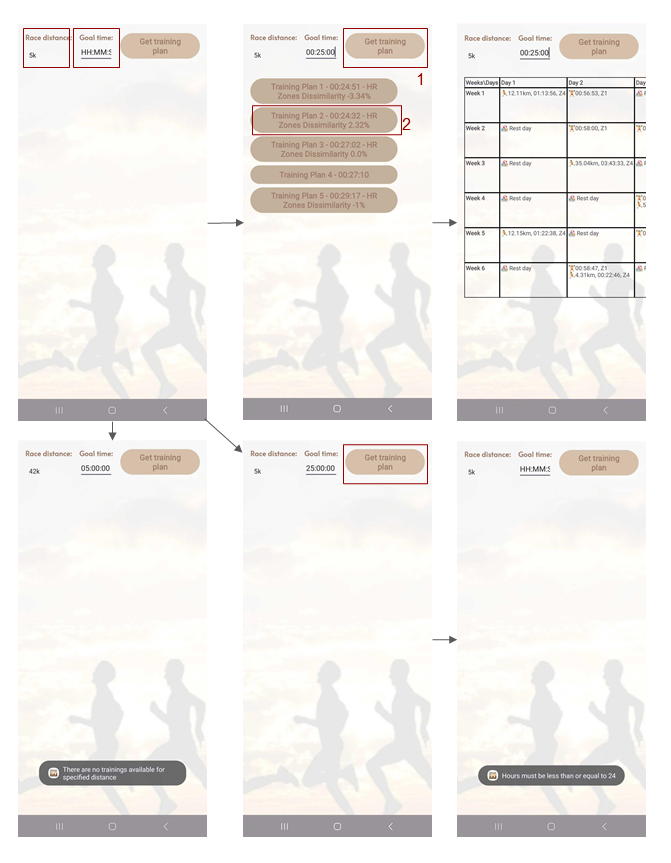
\includegraphics[scale=0.88]{assets/pictures/usecases_flows/training_plan_flow.png}
    \caption{Приказ тока случаја употребе за генерисање плана тренинга}
  \label{pic:training-plan-flow}
\end{figure}


%%%%

\newpage
\subsection*{Предикција резултата на наредној трци}
\begin{longtable}{p{0.23\linewidth} p{0.77\linewidth}}
 \hline
 \textit{\textbf{Актери}} & Корисник, систем (клијентска и серверска апликација) \\
\hline

\textit{\textbf{Предуслови}} & Корисник је пријављен на апликацију \\
 \hline
\textit{\textbf{Постуслови}} & Корисник је добио предикцију резултата на следећој трци или одговарајућу поруку \\
 \hline
 \textit{\textbf{Главни ток}} &  
    \begin{enumerate}
        \item Корисник са главног менија бира опцију за приказивање предикције времена на следећој трци кликом на дугме
        \textit{Predict your race results}
        \item Корисник бира дистанцу трке
        \item Корисник притиска дугме \textit{PREDICT RACE TIME}
        \item Клијентска апликација шаље захтев серверској за добијање предикције времена на следећој трци
        \item Систем приказује предикцију времена на следећој трци или поруку да корисник нема доступне информације на тркама у Републици Србији или доступну информацију за одабрану дистанцу
    \end{enumerate}\\
 \hline
\textit{\textbf{Алтернативни ток}} & Уколико је приликом захтева настала грешка, корисник се обавештава о грешци и случај употребе се завршава \\
 \hline
 
\end{longtable}

\begin{figure}[H]
  \centering
  \begin{minipage}{0.27\textwidth}
    \centering
    
\includegraphics[width=\textwidth]{assets/pictures/app_screenshots/race_prediction_0.jpg}
  \end{minipage}
  \hfill
  \begin{minipage}{0.27\textwidth}
    \centering
    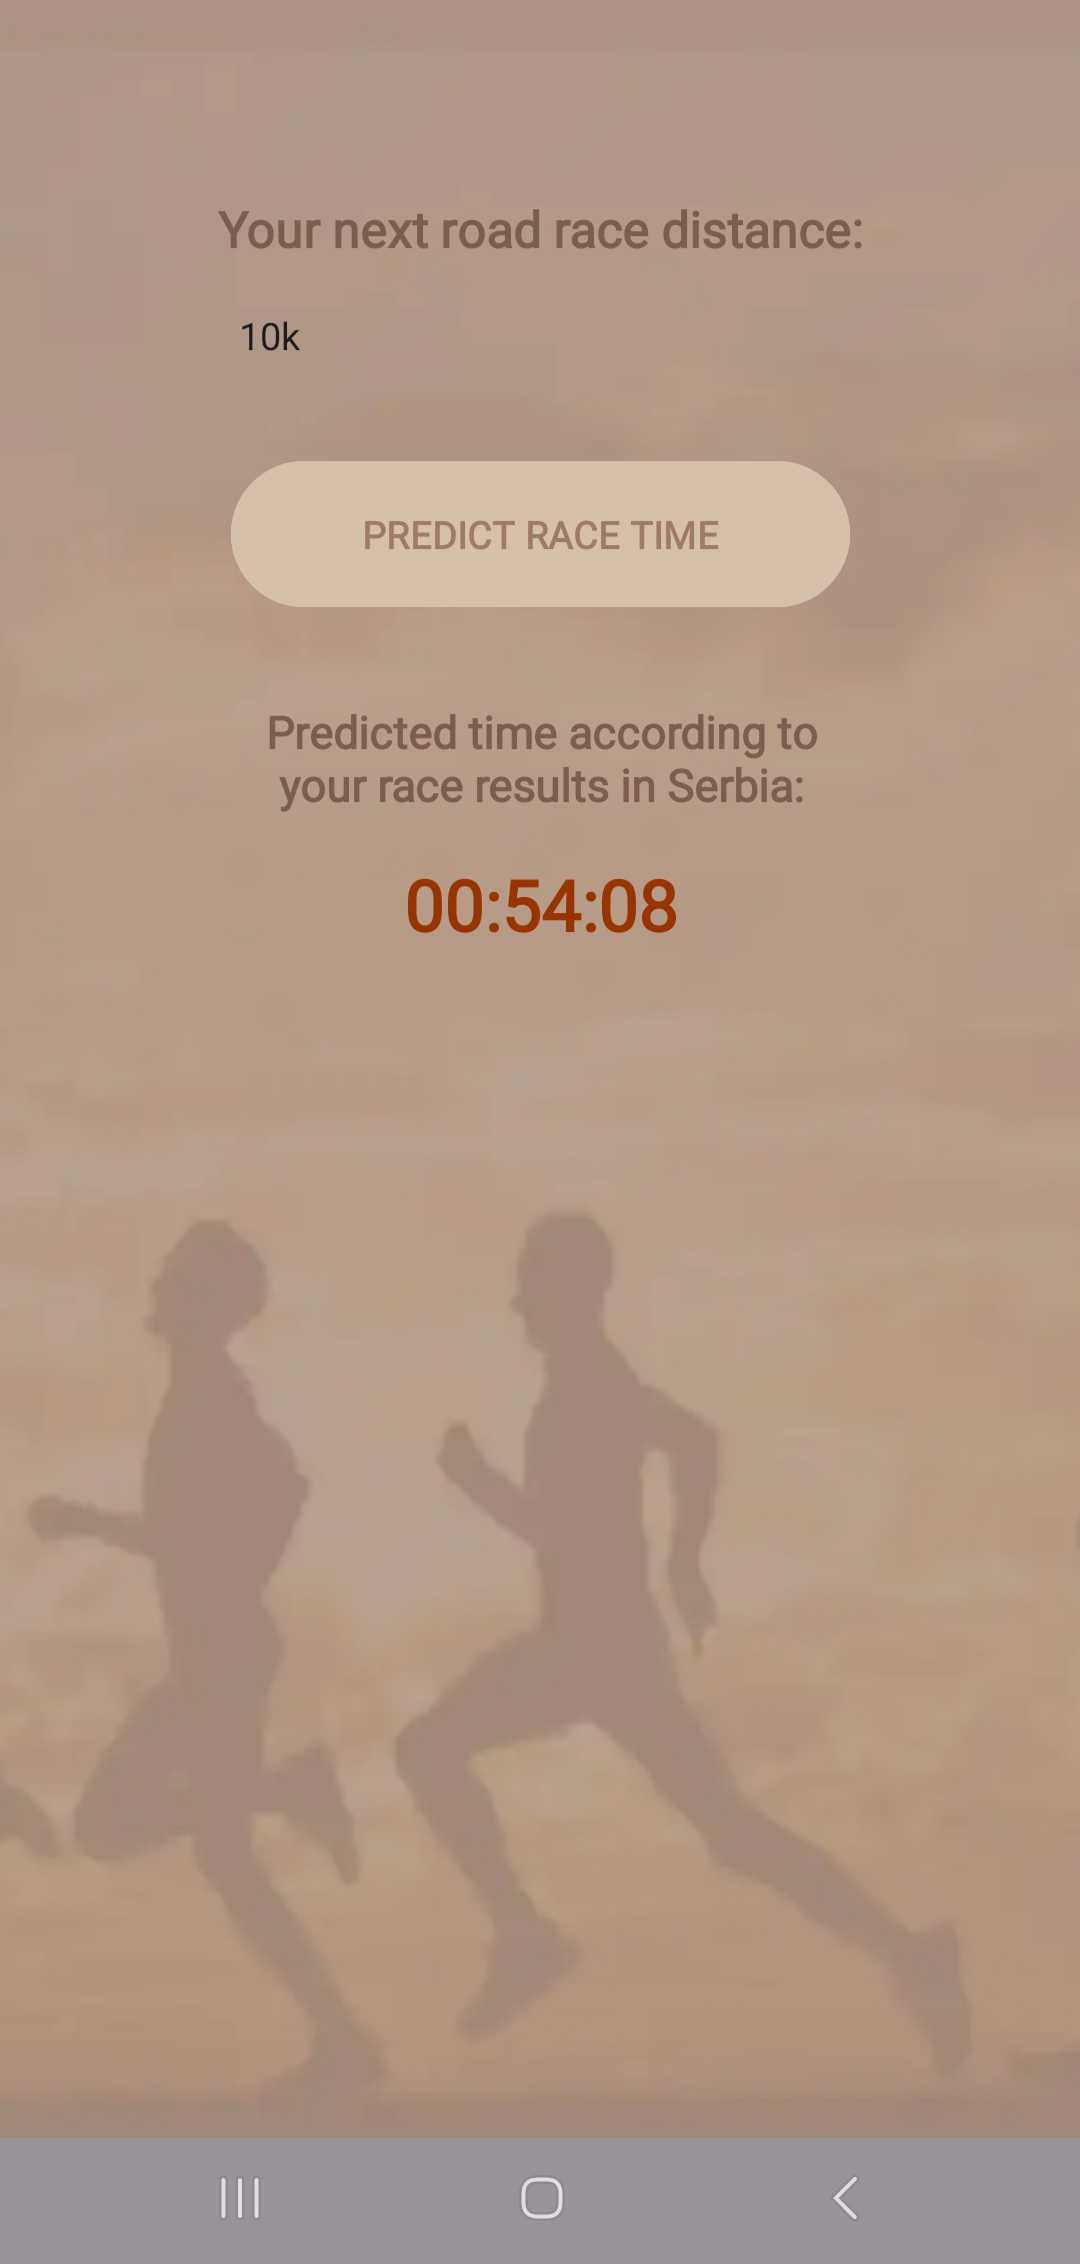
\includegraphics[width=\textwidth]{assets/pictures/app_screenshots/race_prediction_1.jpg}
  \end{minipage}
  \hfill
  \begin{minipage}{0.27\textwidth}
    \centering
    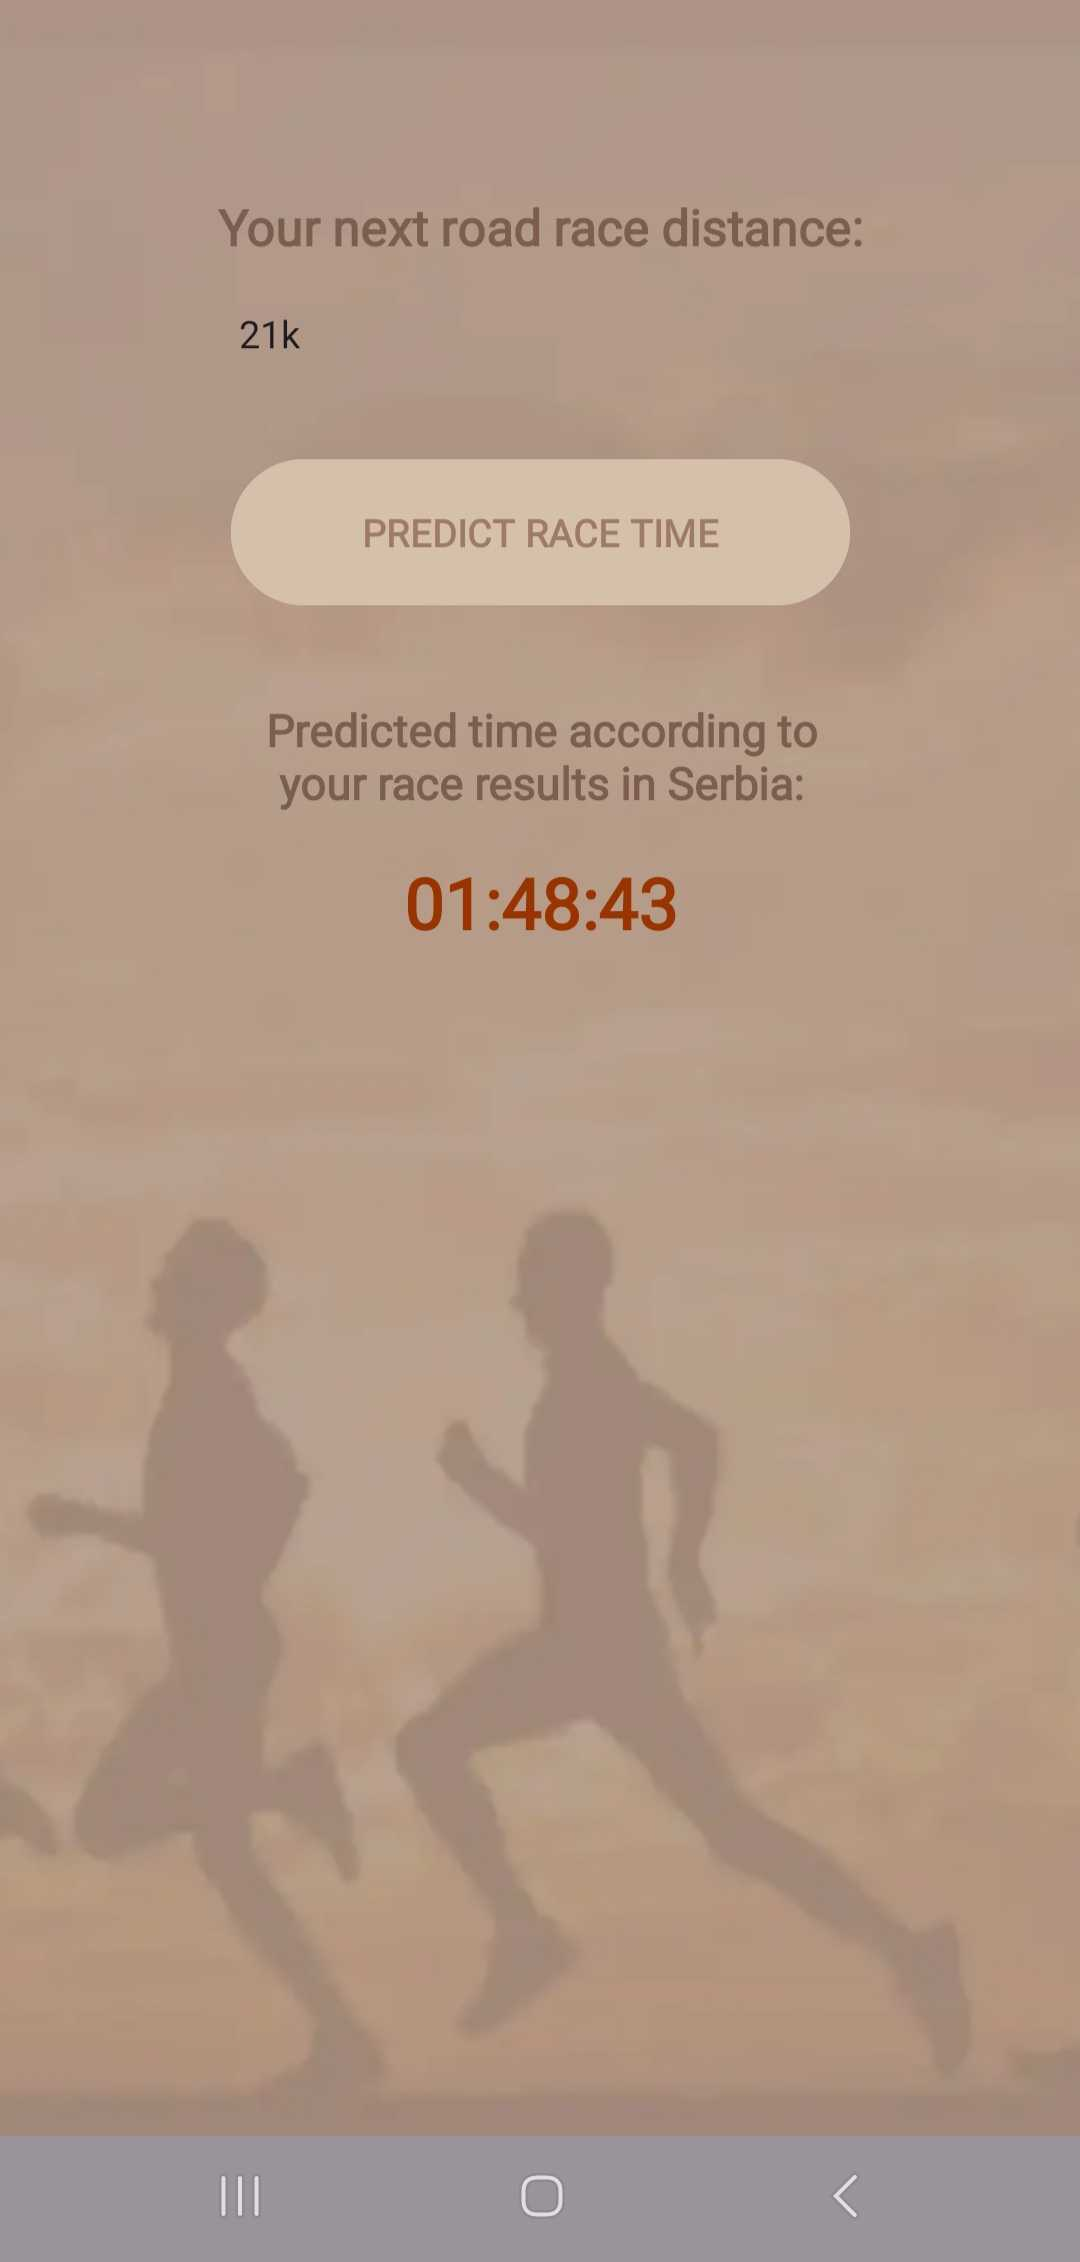
\includegraphics[width=\textwidth]{assets/pictures/app_screenshots/race_prediction_2.jpg}
  \end{minipage}
  \caption{Изглед екрана за предикцију резултата: Иницијални изглед екрана, предикција резултата на трци од 10km и од 21km редом}
  \vfill
  \begin{minipage}{0.25\textwidth}
    \centering
    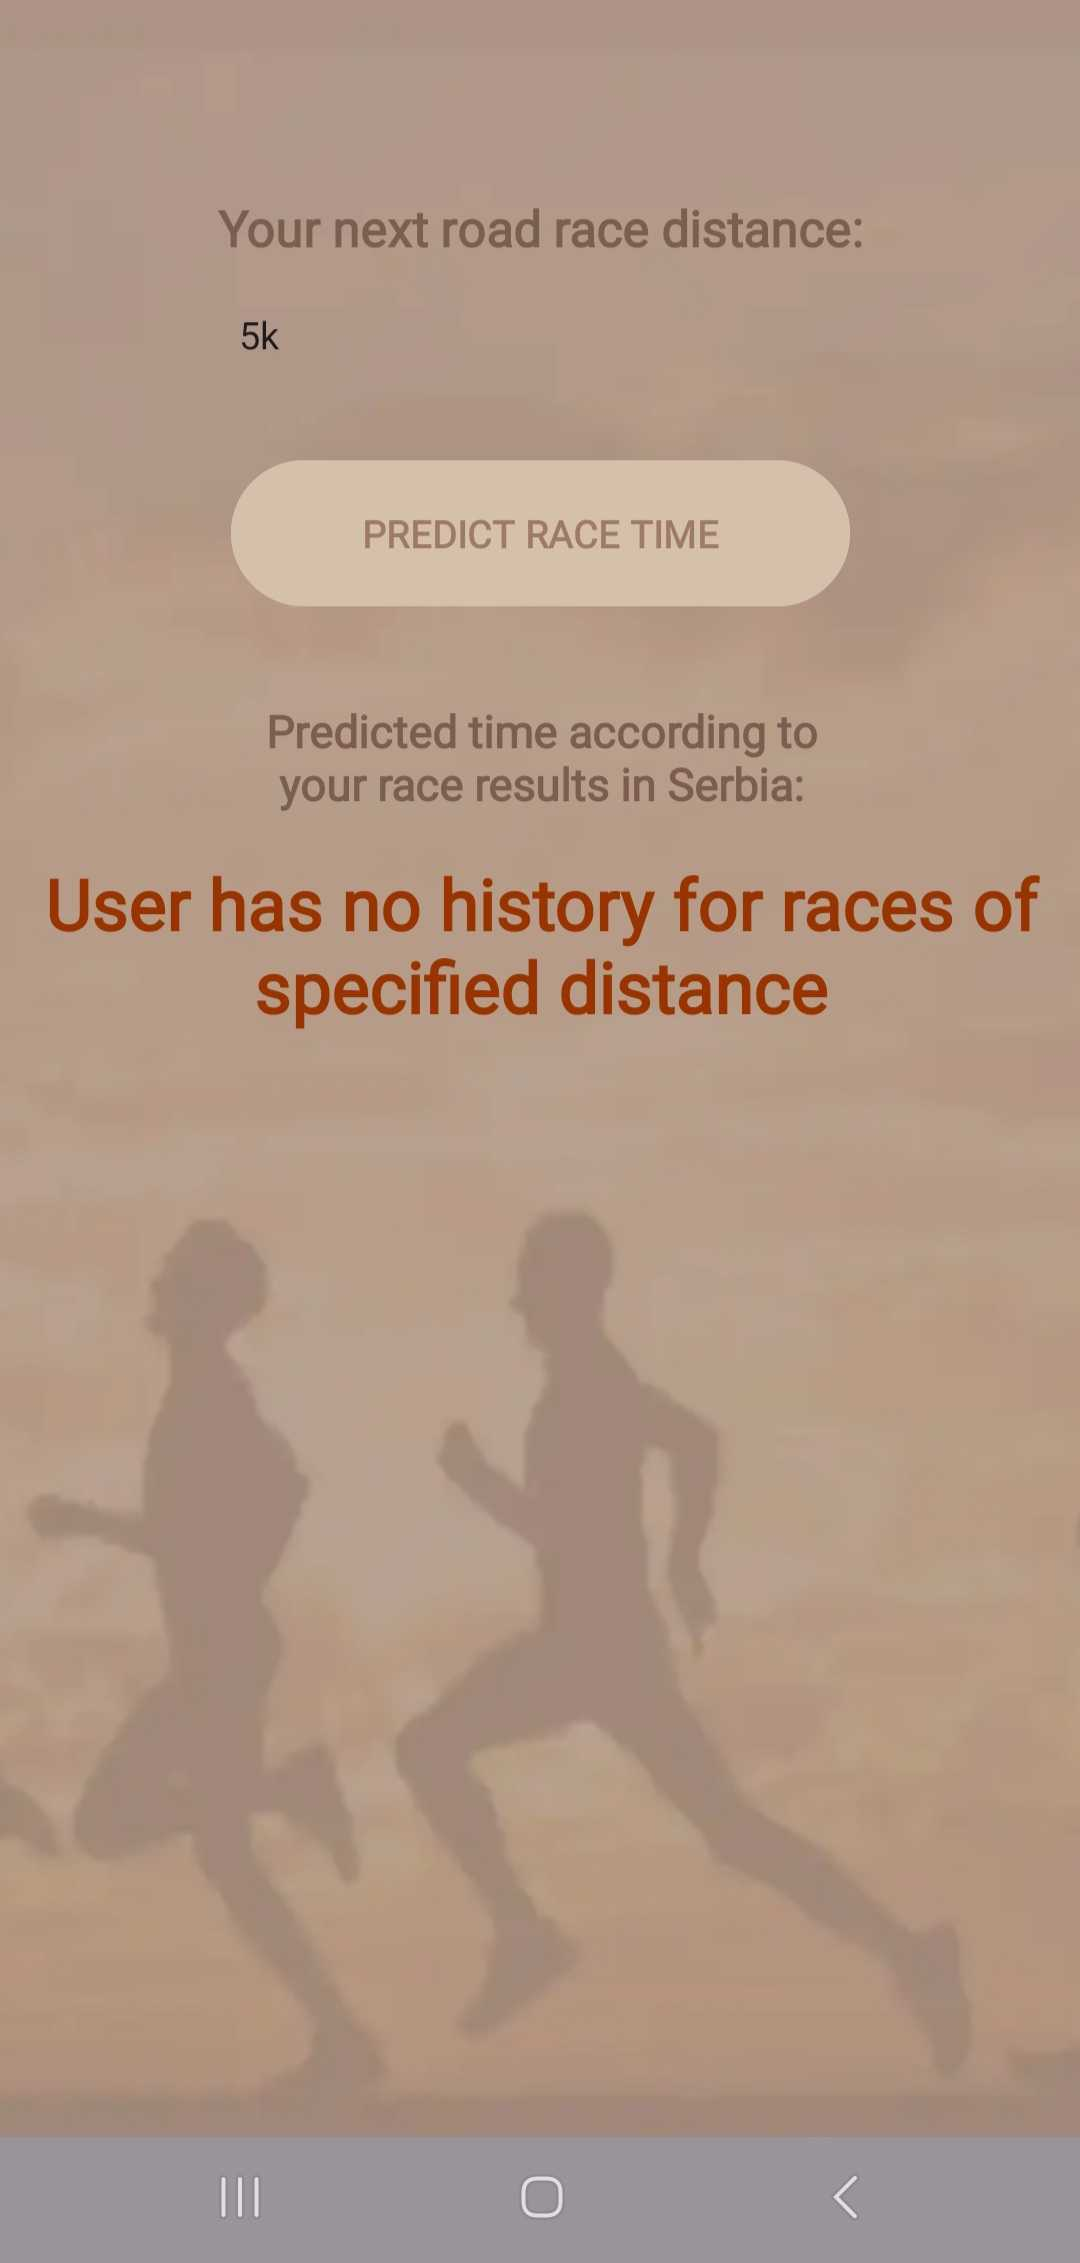
\includegraphics[width=\textwidth]{assets/pictures/app_screenshots/race_prediction_3.jpg}
  \end{minipage}
  \begin{minipage}{0.25\textwidth}
    \centering
    
\includegraphics[width=\textwidth]{assets/pictures/app_screenshots/race_prediction_4.jpg}
  \end{minipage}
  \caption{Изглед екрана за предикцију резултата када корисник нема доступне податке са резултатима на одабраној дистанци и када га нема у бази са резултатима}
  \label{pic:race_prediction}
\end{figure}

\newpage
%%%%%


\subsection*{Месечна статистика тренинга}
\begin{longtable}{p{0.23\linewidth} p{0.77\linewidth}}
 \hline
 \textit{\textbf{Актери}} & Корисник, систем (клијентска и серверска апликација) \\
\hline

\textit{\textbf{Предуслови}} & Корисник је пријављен на апликацију \\
 \hline
\textit{\textbf{Постуслови}} & Корисник је добио месечни извештај о тренинзима за одабрану годину и месец \\
 \hline
 \textit{\textbf{Главни ток}} &  
    \begin{enumerate}
        \item Корисник са главног менија бира опцију за приказивање месечне статистике кликом на дугме
        \textit{Training statistics}
        \item Корисник бира годину и месец
        \item Корисник притиска дугме \textit{Statistics} за генерисање месечне статистике тренинга
        \item Клијентска апликације шаље захтев серверској за добијање месечне статистике
        \item Систем приказује месечну статистику кориснику
    \end{enumerate}\\
 \hline
\textit{\textbf{Алтернативни ток}} & Уколико је приликом захтева настала грешка, корисник се обавештава о грешци и случај употребе се завршава \\
 \hline
 
\end{longtable}

\noindent Ток случаја употребе је приказан на слици \ref{pic:stats-flow}.

\begin{figure}[H]
  \centering
  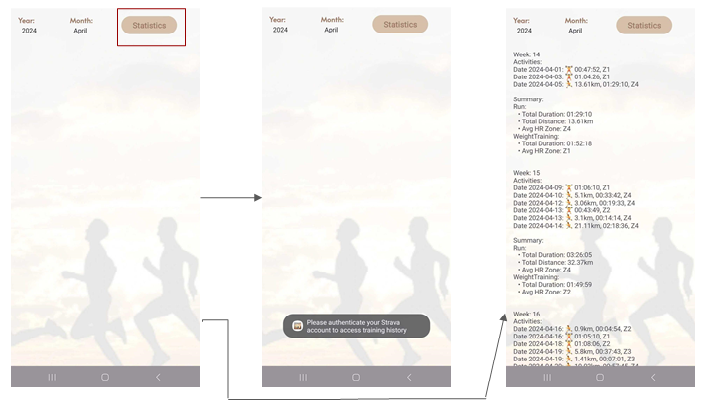
\includegraphics[scale=0.85]{assets/pictures/usecases_flows/stats_flow.png}
    \caption{Приказ тока случаја употребе за генерисање месечне статистике тренинга}
  \label{pic:stats-flow}
\end{figure}


\chapter{Могућа унапређења апликације \textit{Train Wiser}}\label{chapter:improvement-possibilities}

Имплементирана апликација садржи све неопходне карактеристике да би била функционална, у наставку овог поглавља су описани могући начини унапређења како би се њена употреба проширила надградњом постојећих и додавањем нових функционалности.

\paragraph{Додавање личног \textit{online} тренера}

Додавање опције да апликацији могу приступити и лични тренери који би имали могућност да дају план тренинга корисницима и прате њихов напредак кроз приступ тренинзима би допринело проширењу употребе апликације. Било би корисно да апликација олакшава рад тренерима и кроз праћење испуњености задатог тренинга, као и да пружа могућност четовања корисника са тренером и остављања коментара на активностима.

\paragraph{Верификацијa креираног корисничког налога}

Верификација налога путем \textit{e-mail} адресе или броја телефона би допринела побољшању безбедности и поузданости корисничких налога. На овај начин би се утицало на спречавање неовлашћеног приступа и унапређење заштите приватних податкака корисника, што додатно побољшава корисничко искуство и повећава поверење у апликацију.

Увођење верификације путем \textit{e-mail} адресе или броја телефона такође омогућава бржу и лакшу комуникацију са корисницима, било да је реч о постављању нове лозинке у случају да је тренутна заборављена, слању важних обавештења или обезбеђивању додатних слојева сигурности путем двофакторске аутентификације.

\paragraph{Ограничење броја захтева по кориснику у одређеном временском периоду}

Да би се спречило преоптерећење серверске апликације захтевима корисника, корисно је увести ограничење количине захтева у одређеном временском периоду. Ово доприноси одржавању стабилности система, што резултира бржим и стабилнијим одговором на захтеве корисника. Ограничење броја захтева спречава злоупотребе као што су \textit{DDoS} напади\footnote{\textit{DDoS} напад онемогућава приступ интернет услузи преплављивањем многобројним захтевима, трошећи њен капацитет и онемогућавајући одговор на легитимне захтеве} \textit{(Distributed Denial of Service)} чиме се побољшава безбедност апликације. Такође, овакво ограничење олакшава праћење и анализу корисничког понашања, идентификацију аномалија и благовремено реаговање на потенцијалне проблеме.

\paragraph{Прављење статистике са пласманом за трке}

Подаци са резултатима трка у Републици Србији би такође могли да се искористе за праћење потребног времена за одговарајући пласман одређене трке кроз године и процену које место би корисник заузео са тренутним најбољим личним резултатом или за резултат који планира да проба да оствари на наредној трци.


\paragraph{Увођење алгоритма машинског учења за предикцију резултата на трци и предлагање тренинга}

У оквиру процеса израде апликације, направљен је \textit{LSTM} модел који ради над подацима са резултатима трка у Републици Србији. Модел је на улазу добијао претходне три трке корисника и закључивао резултат на четвртој исте дистанце. Међутим, како је просечан број трка по кориснику недовољан за обуку оваквог модела, модел је давао велике грешке. Са оваквим решењем се може пробати у случају доступности већег броја података или применом другачијих алгоритама. 

Такође, направљен је и \textit{LSTM} модел за предлагање тренинга за остваривање очекиваног резултата на одређеној дистанци који на основу дистанце и циљног резултата који се добијају на улазу, врађа секвенцу од 60 низова величине 4 који представљају план тренинга. 

Поступак формирања скупа података је био извоз базе података у \textit{CSV} фајл помоћу имплементиране \textit{Django} команде \texttt{export\_to\_csv}, који се даље учитавао са библиотеком \textit{Pandas} како би се оформиле секвенце. За сваку трку из базе података која је дистанце 5, 7, 7.7, 10, 21 или 42 километара се узимао скуп тренинга из претходних 60 дана. Тренинзи су представљени секвенцом са типом тренинга, дужином, дистанцом и просечном зоном срчаног пулса, док за дане без тренинга све елементе секвенце садрже нулу.

Овакав модел би могао да се дотренирава са подацима корисника који се пријављују на апликацију и ауторизују је на апликацији \textit{Strava}. Међутим, због тренутне недовољне количине података да би модел давао релевантне резултате, овај модел није убачен у \textit{API} серверске апликације. Уместо тога, користио се приступ са предлагањем тренинга корисника који је остварио најближи резултат циљаном.



\chapter{Закључак}\label{chapter:summary}


Овај рад је на примеру апликације за вежбаче обрадио концепте развоја апликација за оперативни систем \textit{Android} и апликација \textit{Python} програмског језика које користе оквире \textit{Django} и \textit{Django REST Framework}. У раду је након теоријског увода у поменуте технологије дат детаљан опис имплементације
и употребе креиране апликације. Такође, детаљно су представљене остале технологије и алати коришћени при развоју, попут протокола \textit{OAuth 2.0}, оквира \textit{Scrapy} за екстракцију података, \textit{Cron} послова, концепта мрежних кука итд. Рад садржи сумиране препоруке за наредне фазе унапређења апликације.

Креирана апликација доприноси пољу спортских апликација за трчање кроз детаљну статистику о тренинзима, предлагање различитих планова тренинга припреме за одређену тркачку дистанцу и предикцијом временског резултата на наредној трци. Коришћењем поменутих технологија, омогућен је рад са корисничким подацима, њихова анализа, обрада и интерпретација у складу са потребама корисника. Апликација представља пример начина за рад са корисничким подацима и приказује како они могу допринети бољем раду програма и корисничком искуству, разноврсност корисничких података доприноси бољем раду алгоритама апликације. У контексту рада са корисничким подацима, даља побољшања се огледају како у унапређењу постојећих функционалности новим алгоритмима, тако и у додавању нових приступа при раду са постојећим подацима.

Апликација овог типа може служити као темељ за изградњу апликација које раде са корисничким подацима, апликација које користе ауторизацију спољних налога са других сервиса, као и за развој других типова апликација које су базиране на оперативном систему \textit{Android} или користе оквире \textit{Django} и \textit{Django REST Framework}.


% ------------------------------------------------------------------------------


% ------------------------------------------------------------------------------
% Literatura
% ------------------------------------------------------------------------------
\literatura

% ==============================================================================
% Završni deo teze i prilozi
\backmatter
% ==============================================================================

% ------------------------------------------------------------------------------
% Biografija kandidata
\begin{biografija}

\end{biografija}
% ------------------------------------------------------------------------------

\end{document} 